\documentclass[journal]{IEEEtran}
\usepackage{orcidlink}
\usepackage{cuted} 
\usepackage{subcaption}
\usepackage{cite}
\usepackage{amsmath}
\usepackage{graphicx}
\usepackage{url}
\usepackage{booktabs}
\usepackage{xcolor}
\usepackage[normalem]{ulem}
\usepackage[compatibility=false]{caption} 
\usepackage{xurl}
\hyphenation{op-tical net-works semi-conduc-tor}

\begin{document}

\title{From Articles to Publishers: Aggregating Language Model Predictions for News Source Reliability Inference}
%Publisher Reliability Inference via Aggregated Article-Level Predictions

\author{John~Bianchi\,\orcidlink{0009-0006-2582-1480},
        Manuel~Pratelli\,\orcidlink{0000-0002-9978-791X},
        Fabio~Pinelli\,\orcidlink{0000-0003-1058-6917},
        and Marinella~Petrocchi\,\orcidlink{0000-0003-0591-877X}%
\thanks{J. Bianchi is with the IMT School for Advanced Studies Lucca, 55100 Lucca, Italy (e-mail: john.bianchi@imtlucca.it).}%
\thanks{M. Pratelli is with the Institute of Informatics and Telematics, National Research Council (IIT-CNR), 56124 Pisa, Italy (e-mail: manuel.pratelli@iit.cnr.it).}%
\thanks{F. Pinelli is with the IMT School for Advanced Studies Lucca, 55100 Lucca, Italy (e-mail: fabio.pinelli@imtlucca.it).}%
\thanks{M. Petrocchi is with the Institute of Informatics and Telematics, National Research Council (IIT-CNR), 56124 Pisa, Italy, and with the IMT School for Advanced Studies Lucca, 55100 Lucca, Italy (e-mail: marinella.petrocchi@iit.cnr.it).}%
\thanks{Corresponding author: John Bianchi.}%
\thanks{This work is partially supported by IIT-CNR internal project SIMULARE `SIMULAzione delle Reazioni alla disinformazionE con LLM'.}%
}

\markboth{IEEE Transactions on Computational Social Systems,~Vol.~XX, No.~X, XXXX~2026}%
{Bianchi \MakeLowercase{\textit{et al.}}: Aggregating Language Model Predictions for News Source Reliability Inference}

\maketitle

\begin{abstract}
Traditionally, the reliability of news publishers is assessed by expert organisations that evaluate editorial practices, transparency and factual standards at source. When this process is translated into a computational approach, the problem is often formulated at the level of individual articles, with models being trained on a set of pre-labelled articles and their performance being evaluated in a test phase. % the problem is often formulated at the article level by evaluating models in settings where publishers may overlap between training and test data, leading to inflated generalization performance.
In this work, we investigate news source reliability inference as a source-level prediction problem. We propose a two-stage framework in which transformer-based language models first estimate the reliability of individual articles and subsequently aggregate article-level predictions to infer the reliability of previously unseen publishers.
To approximate realistic deployment conditions, we enforce a strict publisher-disjoint evaluation protocol, ensuring that no publisher appears in both training and test sets.
Experiments on 19,476 political news articles from 439 English-language publishers labeled with NewsGuard reliability ratings show that aggregation substantially improves robustness and performance, increasing accuracy from approximately 0.60 at the article level to 0.69 at the publisher level.
Finally, we analyze how prediction errors vary across political orientations, revealing statistically significant associations between political leaning and misclassification patterns.
Overall, our findings show that publisher reliability can be inferred from aggregated textual signals alone, supporting scalable and content-based approaches to automated news source assessment.


% Manual assessment of news outlet reliability is typically conducted by expert raters who evaluate aspects like the outlet's ownership, editorial practices, and content quality. Although effective, this process is resource-intensive and difficult to scale. In this study, we investigate whether modern language models can support this task by predicting the reliability level of a news source from the textual content of its articles. We formulate the problem as a five-level ordinal classification aligned with ratings used by professional journalistic organizations and train transformer-based models on a large dataset of articles labeled with publisher reliability scores. To approximate real-world deployment, we evaluate model performance under a strict cross-publisher setting, where all test articles originate from news outlets unseen during training. The results show that language models achieve approximately 0.60 article-level accuracy under strict cross-publisher evaluation, rising to 0.69 at the publisher level through aggregation. We also find statistically significant associations between political leaning and misclassification patterns. Overall, our findings highlight the potential of content-based approaches for scalable, automated assessment of news outlet reliability and underscore the importance of auditing model behavior across politically diverse media ecosystems.
\end{abstract}

\begin{IEEEkeywords}
News source reliability, 
Publisher reliability inference, 
Transformer-based text classification, 
Cross-publisher generalization, 
Reliability aggregation, 
Political bias analysis.
\end{IEEEkeywords}

\IEEEpeerreviewmaketitle




% \section{Introduction}
% \label{sec:intro}
% In recent decades, the digital transformation of the media ecosystem has profoundly altered the production and circulation of information. While broader participation has expanded access to news, it has also facilitated the spread of misleading and low-quality content, increasing the need for reliable mechanisms to assess the trustworthiness of news sources \cite{Bowman2003, Jemielniak2020}.

% Several professional initiatives, including NewsGuard, the Global Disinformation Index, and Media Bias Fact Check, evaluate publishers according to journalistic standards such as transparency, editorial practices, and factual accuracy. Despite methodological differences, these systems exhibit substantial convergence, providing a stable foundation for reliability labeling ~\cite{lin2023high,DBLP:conf/icwsm/PratelliP22}. However, manual assessment remains resource-intensive and difficult to scale across rapidly evolving media ecosystems.

% This study investigates whether publisher reliability can be inferred directly from article texts. We frame the problem as a five-level ordinal classification task aligned with NewsGuard ratings and evaluate transformer-based models on a large corpus of political news articles. Unlike prior work that often mixes articles from the same outlets across training and test sets, we adopt a strict publisher-disjoint protocol: all test articles originate from previously unseen publishers. This setting prevents label leakage and simulates real-world deployment, where systems encounter new sources.

% Further, we introduce a source reliability profiling task that aggregates article predictions via majority voting to estimate publisher-level ratings. This approach reflects practical scenarios in which reliability is assessed at the domain level rather than at the level of individual articles.

% Finally, we examine whether model errors vary systematically across political orientations. By combining error-rate analysis, directional bias metrics, and statistical testing, we assess the interaction between ideological leaning and reliability prediction.

% Our contributions are threefold. First, we construct a large-scale dataset of 19,476 political news articles from 439 English-language publishers labeled with professional reliability scores. Second, we demonstrate that transformer-based models generalize to previously unseen publishers under a strict evaluation protocol, achieving 
% %around 0.60 article-level accuracy and 
% up to 0.69 publisher-level accuracy when predictions on single articles are aggregated. When allowing near-miss errors between adjacent reliability levels, performance increases further, % (
% %up to 0.84 at the article level and 
% up to 0.88 at the publisher level. Third, we provide empirical evidence that misclassification patterns are not independent of political leaning, with statistically significant associations between error rates and ideological orientation ($\chi^2$ test, p $< 10^{-250}$, Cramér's $V \approx 0.25$--$0.29$). This underscores the importance of bias-aware evaluation in automated credibility assessment systems.


\section{Introduction}
In contemporary digital media ecosystems, assessing the reliability of news publishers has become increasingly important for limiting the spread of misleading or low-quality information. Professional organizations such as NewsGuard, the Global Disinformation Index, and Media Bias Fact Check evaluate news outlets according to journalistic standards including transparency, editorial accountability, factual accuracy, and correction practices. Despite methodological differences, these systems exhibit substantial convergence, providing a stable foundation for reliability labeling~\cite{lin2023high,DBLP:conf/icwsm/PratelliP22}. Importantly, these assessments are performed at the level of the publisher rather than at the level of individual articles.

A large body of computational approaches to misinformation and credibility assessment formulates the problem as an article-level classification task~\cite{pandolfi2020automatic,Przybyla2021plugin,DBLP:journals/corr/abs-2410-21360,DBLP:journals/dbsk/AdjiLS26}. Existing systems typically attempt to determine whether a single article is credible, misleading, or unreliable based on linguistic patterns, stylistic signals, or neural representations. While effective in controlled settings, this formulation only partially reflects the actual structure of professional reliability assessment, where reliability is considered a persistent property of the news source emerging across multiple publications rather than an intrinsic property of isolated articles.

This mismatch introduces an important methodological challenge. Individual articles provide only partial and noisy evidence about the overall reliability of the publisher that produced them. Even highly reliable outlets may occasionally publish lower-quality content, while unreliable publishers may produce articles that appear factually plausible in isolation. Consequently, estimating publisher reliability from single articles is inherently unstable. A more realistic formulation instead consists in inferring source-level reliability by aggregating evidence collected across multiple articles belonging to the same publisher.

A second limitation of prior work concerns evaluation methodology. Existing studies evaluate article reliability using datasets in which labels are derived from publisher-level annotations and where evaluation does not explicitly enforce publisher-disjoint splits, see, e.g., ~\cite{burdisso-etal-2024-reliability, DBLP:journals/dbsk/AdjiLS26,batDataset}. 
% Because article labels are typically inherited from publisher-level annotations, this setup introduces substantial leakage of publisher identity and may artificially inflate model performance. 
Under these conditions, models can partially memorize publisher-specific patterns rather than learning transferable indicators of reliability~\cite{azizov-etal-2024-safari,verhoeven2025yesterday}.

In this work, we address these limitations by reformulating news reliability assessment as a publisher-level inference problem. We propose a two-stage framework in which transformer-based language models first estimate the reliability level of individual articles and subsequently aggregate article-level predictions to infer the reliability of previously unseen publishers. To approximate realistic deployment conditions, we enforce a strict publisher-disjoint evaluation protocol, ensuring that no publisher appears in both training and test sets.

More specifically, we frame article reliability estimation as a five-level ordinal classification problem aligned with NewsGuard ratings and evaluate four transformer-based architectures under strict cross-publisher generalization. We then study how aggregating predictions across collections of articles improves the estimation of publisher reliability. Finally, we analyze the relationship between political orientation and model errors, providing a bias-aware evaluation of the proposed framework.

Our contributions are fourfold:

\begin{enumerate}
    \item 
We reformulate news reliability assessment as a source-level inference problem, where publisher reliability is estimated by aggregating predictions from multiple articles.
\item We introduce a strict publisher-disjoint evaluation protocol that prevents source leakage and measures generalization to previously unseen publishers.
\item We construct a large-scale dataset of 19,476 political news articles from 439 English-language publishers labeled with NewsGuard reliability scores.
\item We show that aggregating article-level predictions substantially improves reliability estimation, achieving up to 0.69 publisher-level accuracy on unseen sources.\end{enumerate}


% In recent decades, the digital transformation of the media ecosystem has profoundly altered the production and circulation of information. While broader participation has expanded access to news, it has also facilitated the spread of misleading and low-quality content, increasing the need for reliable mechanisms to assess the trustworthiness of news sources~\cite{bowman2003, Jemielniak2020}.

% Several professional initiatives, including NewsGuard, the Global Disinformation Index, and Media Bias Fact Check, evaluate publishers according to journalistic standards such as transparency, editorial practices, and factual accuracy. Despite methodological differences, these systems exhibit substantial convergence, providing a stable foundation for reliability labeling~\cite{lin2023high,DBLP:conf/icwsm/PratelliP22}. However, manual assessment remains resource-intensive and difficult to scale across rapidly evolving media ecosystems.

% A growing body of research has explored automatic approaches to misinformation detection and credibility assessment. Early work primarily focused on article-level classification, aiming to detect misleading content using linguistic patterns or neural architectures. More recent studies have shifted attention toward the reliability of the publisher itself, leveraging signals such as social networks, metadata, or external ratings. However, two key limitations remain.

% First, many approaches rely on signals that are not always available or scalable, such as user interactions, network structure, or expert annotations. Second, and more critically, evaluation protocols often allow articles from the same publishers to appear in both training and test sets, leading to implicit leakage of publisher identity and overestimating model generalization.

% As a result, it remains unclear whether \textit{article text alone} encodes sufficiently robust signals to infer publisher reliability, particularly in realistic settings where models must generalize to entirely unseen sources.

% In this work, we address this gap by investigating whether transformer-based models can predict the reliability of news publishers using only article text, under a strict cross-publisher evaluation protocol. We frame the task as a five-level ordinal classification problem aligned with NewsGuard ratings and evaluate performance in a setting where all test articles originate from previously unseen publishers.

% To further approximate real-world deployment, we introduce a source-level inference task, where article-level predictions are aggregated to estimate publisher reliability. In addition, we analyze how model errors vary across political orientations, providing a bias-aware evaluation of reliability prediction.

% Our contributions are threefold:
% \begin{itemize}
%     \item We construct a large-scale dataset of 19,476 political news articles from 439 English-language publishers labeled with professional reliability scores.
%     \item We show that transformer-based models can predict publisher reliability from article text alone and generalize to unseen sources under a strict publisher-disjoint protocol, achieving up to 0.69 accuracy at the publisher level.
%     \item We provide a systematic analysis of model bias, showing statistically significant associations between political leaning and misclassification patterns.
% \end{itemize}

% Overall, our findings demonstrate that content-based signals capture meaningful and transferable indicators of publisher reliability, offering a scalable complement to expert-driven assessments.


\section{Related Work}

The quality of online news has been widely studied in computational social science and natural language processing. Early work focused on article-level classification, detecting misleading content through linguistic features, supervised models, or deep neural architectures~\cite{pandolfi2020automatic}, often without explicitly considering the role of the publisher.

\paragraph{Publisher Reliability as a Core Dimension} A parallel line of research shifts the focus to the reliability of news publishers. This concept is described using terms such as \emph{reliability}, \emph{trustworthiness}, and \emph{credibility}, which capture whether a source adheres to journalistic standards and is perceived as informative rather than misleading~\cite{digitalmedia2007,infodisorder2017,10.1145/302979.303001}. Empirical studies show that source reputation strongly influences perceived information quality~\cite{doi:10.1080/07421222.2019.1628921}. 

\paragraph{Different signals to estimate publisher reliability} Computational approaches model publisher reliability using different types of signals. Some rely on textual features and stylistic patterns~\cite{przybyla2021classification}, while others incorporate external information such as user interactions, social networks, and other metadata~\cite{bazmi2023multi,DBLP:conf/ecir/PratelliSP25,DBLP:conf/icwsm/WilliamsCC25,DBLP:journals/jdiq/LongoZCZC25}. In addition, journalistic rating systems such as NewsGuard, the Global Disinformation Index, and Media Bias/Fact Check show strong agreement and are commonly used as ground truth for automated models~\cite{lin2023high,DBLP:conf/icwsm/PratelliP22}. Recent work further explores textual and LLM-based approaches to reliability estimation~\cite{10.1145/3770077,nakov2024survey,yang2023large,Leite2025}.

\paragraph{Datasets and Cross-Domain Generalization} Datasets with explicit publisher reliability labels remain limited. Bohacek et al.~\cite{bohavcek2022fine} introduce a Czech dataset with four reliability levels, while Adji et al.~\cite{DBLP:journals/dbsk/AdjiLS26} reconstruct the BAT corpus~\cite{batDataset} by recovering article texts and consolidating reliability categories into a standardized benchmark. More recent work highlights the challenge of generalization across domains and publishers~\cite{azizov-etal-2024-safari,burdisso-etal-2024-reliability,verhoeven2025yesterday}, showing that model performance degrades under distribution shifts.

Existing approaches may evaluate models in settings where training and test data share the same publishers. As a result, models may implicitly learn publisher-specific patterns rather than generalizable signals, leaving open whether reliability can be inferred from article text alone and transferred to unseen sources.

\paragraph{Our contribution} In contrast, we focus exclusively on textual content and enforce a strict publisher-disjoint evaluation protocol. We show that publisher reliability can be inferred from article text through aggregation of article-level predictions under a strict publisher-disjoint protocol.

% \section{Related Work}

% The quality of online news has been widely studied in computational social science and NLP. Early work focused on article-level classification, detecting misleading content through linguistic features and neural models~\cite{pandolfi2020automatic}, often without considering the role of the publisher.

% \textit{Publisher Reliability.}
% A parallel line of research shifts the focus to the reliability of news publishers. This concept is described using terms such as \emph{reliability}, \emph{trustworthiness}, and \emph{credibility}, which all capture whether a source adheres to journalistic standards and is perceived as informative rather than misleading~\cite{digitalmedia2007,infodisorder2017,10.1145/302979.303001}. Empirical studies show that source reputation strongly influences perceived information quality~\cite{doi:10.1080/07421222.2019.1628921}.

% Computational approaches model publisher reliability using different signals. Some leverage stylistic features of articles~\cite{przybyla2021classification}, while others incorporate external information such as user interactions or source metadata~\cite{bazmi2023multi}. In addition, journalistic rating systems (e.g., NewsGuard, GDI, MBFC) show strong agreement and are commonly used as ground truth~\cite{lin2023high,DBLP:conf/icwsm/PratelliP22}. Recent work also explores LLM-based estimation and textual cues for reliability assessment~\cite{10.1145/3770077,nakov2024survey}. However, many of these approaches rely on external signals beyond article text.

% \textit{Datasets and Generalization.}
% Datasets with explicit publisher reliability labels remain limited. Bohacek et al.~\cite{bohavcek2022fine} introduce a Czech dataset, while Adji et al.~\cite{DBLP:journals/dbsk/AdjiLS26} reconstruct the BAT corpus~\cite{batDataset} with full article texts and standardized labels. More recent work highlights the challenge of generalization across domains and publishers~\cite{azizov-etal-2024-safari,burdisso-etal-2024-reliability,verhoeven2025yesterday}, showing performance drops under distribution shifts.

% However, many evaluation protocols do not enforce strict separation between publishers in training and test sets. As a result, models may rely on publisher-specific patterns, leaving open whether reliability prediction can generalize to unseen sources using textual content alone.

% \textit{Relation to Our Contribution.}
% Prior work often depends on external signals or evaluates models on overlapping publishers. In contrast, we focus exclusively on article text and enforce a publisher-disjoint evaluation setting. We show that transformer-based models can predict NewsGuard’s five-level reliability scale and generalize to previously unseen sources, demonstrating the potential of content-based approaches for scalable reliability assessment.

% \textit{Reliability from Social Interactions and User Behavior.}
% Beyond textual cues, reliability can emerge from social dynamics.
% The TROPIC tool \cite{DBLP:conf/ecir/PratelliSP25} infers publisher reliability based on user interactions on social platforms. It constructs a network of sources and their audiences in order to estimate reliability for news outlets that have not previously been labeled. 
% \textcolor{blue}{Williams et al.~\cite{DBLP:conf/icwsm/WilliamsCC25} further show that combining webgraph structure with large-scale social media co-mention patterns improves the classification of unreliable  information domains, outperforming both LLM-based and content-agnostic baselines. Along similar lines, Longo et al.~\cite{DBLP:journals/jdiq/LongoZCZC25} show that metadata richness, measured via FAIR data principles, correlates with reliability scores assigned by external fact-checking organizations, suggesting that structural properties of a news source's data publication practices carry reliability signals beyond article content.} These approaches demonstrate how ecosystem-level signals can complement content-based assessments.

% \textit{LLM-Based Assessment.}
% LLMs have recently introduced a new paradigm for estimating publisher reliability. Yang and Menczer in \cite{yang2023large} show that state-of-the-art LLMs can produce reliability ratings for news outlets with high inter-model agreement, although alignment with human expert ratings varies and political bias may affect outcomes.
% Leite et al. \cite{Leite2025} introduce a weakly supervised approach in which LLM-generated credibility indicators are used to train veracity classification systems. They demonstrate that predictions about credible sources can be used to improve performance in subsequent tasks.
% Other recent LLM-based approaches estimate source reliability from content alone or by combining weak supervision with media profiling \cite{10.1145/3770077,nakov2024survey}.

% \textit{Relation to Our Contribution.}

% Despite the growing body of work on publisher reliability, existing approaches typically rely on external signals such as social networks, metadata, or pre-existing source ratings, and often evaluate models in settings where training and test data share the same publishers. As a result, it remains unclear whether article text alone encodes sufficiently robust signals to generalize across previously unseen outlets.

% Our work addresses this limitation by focusing exclusively on textual content and explicitly enforcing a publisher-disjoint evaluation protocol. We show that transformer-based models can predict NewsGuard’s five-level reliability scale using only article text, and that these predictions generalize to entirely new sources. This provides evidence that content-based signals capture transferable indicators of publisher reliability, offering a scalable complement to expert-driven assessments.


\section{Problem Definition and Methodology}
\label{sec:problemDef}

\subsection{Problem definition}\label{subsec:problemdef}
We formulate the problem as `News Source Reliability Inference', whose objective is to estimate the reliability level of a publisher from its published content. Because publishers are observed through collections of articles, we decompose the problem into two stages: (i) Article-level reliability estimation and (ii) Publisher-level reliability inference through aggregation.

Let \(A = \{a_1, a_2, \ldots, a_n\}\) be a corpus of news articles. Each article \(a \in A\) has a textual representation \(t_a \in \mathcal{T}\) and belongs to a publisher \(p(a) \in P\). 
For a given publisher \(p \in P\), we denote by
\[
A_p = \{\, a \in A \mid p(a) = p \,\}
\]
the set of articles published by \(p\).
Each publisher \(p \in P\) has a fixed reliability level \(r_P(p)\). We use five ordered categories \(L = \{l_1, \ldots, l_5\}\) obtained by binning continuous reliability scores (see Section~\ref{sec:dataset}). Since reliability is a publisher's property, every article inherits its publisher's label: \(r_A(a) = r_P(p(a))\).
Analogously, each publisher \(p \in P\) has a political leaning associated \(o_P(p)\). 
The political leaning of each publisher is inherited by its articles \(a \in A_p\), formally: \(o_A(a) = o_P(p(a))\). The political leaning belongs to a set of 5 possible values \(O = \{\text{Far Left},\text{Slightly Left}, \text{Not Labeled}, \text{Slightly Right}, \text{Far Right} \}\). 
These two inheritance functions are needed since article-level annotation is not available. Notice that political leaning is not used as a model input or prediction target; rather, we retain this annotation to enable a post-hoc analysis of the classifier behavior (see Section~\ref{subsec:politicalBias}).

\paragraph{Stage 1: Article-level reliability estimation} 
We train a classifier \(C_{\text{reliability}}: \mathcal{T} \rightarrow L\) to predict the reliability level of a single article using only its text.

\paragraph{Stage 2: Publisher reliability inference} 

To simulate how a system profiles a new, unseen source, we estimate the publisher-level reliability by aggregating predictions obtained from its articles.
For a given publisher \(p \in P\), we aggregate predictions obtained from the articles in \(A_p\), defining an aggregation function
\[
Agg: L^{|A_{p}|} \rightarrow L
\]
that maps the article-level reliability predictions to a
publisher-level label.
The predicted reliability of publisher \(p\) is then computed as:
\[
\hat{r}_P(p) = Agg\big(\{ C_{\text{reliability}}(a) \mid a \in A_p \}\big).
\]
In~\ref{sec:results} we instantiate \(Agg\) as the mode, corresponding to majority voting. 

A key constraint of our problem formulation follows directly from the inheritance mechanism used to obtain article-level labels. Since each article inherits the reliability label of its publisher, articles originating from the same source are not independently labeled. Consequently, a random split at the article level would lead to severe label leakage, allowing the model to indirectly observe the test labels during training through articles from the same publisher. To address this issue, we enforce a strict separation of publishers between the training and test sets.
Let \(A_{\text{train}} \subset A\) and \(A_{\text{test}} \subset A\) denote
the sets of articles used for training and testing, respectively, with
\(A_{\text{train}} \cap A_{\text{test}} = \emptyset\).

Let \(P_{\text{train}} = \{\, p(a) \mid a \in A_{\text{train}} \,\}\) and
\(P_{\text{test}} = \{\, p(a) \mid a \in A_{\text{test}} \,\}\) be the sets
of publishers associated with the training and test articles.
We enforce that these sets are disjoint:
\begin{equation}\label{eq:publisher_disjoint}
P_{\text{train}} \cap P_{\text{test}} = \emptyset .
\end{equation}

This evaluation protocol ensures that all test articles originate from previously unseen publishers, thereby aligning the evaluation setting with the source-level nature of the ground-truth labels and preventing publisher-specific memorization.

\subsection{Evaluation Metrics and Baselines}\label{subsection:metrics}
We use the same metrics for both article-level and source-level evaluations.

\paragraph{Standard and Macro Metrics} 
We report Accuracy as the ratio of correct predictions. Although the class distribution is relatively stable, there are moderate differences in frequency (e.g., $l_4$ is approximately 2.6 times larger than $l_5$). To ensure that our evaluation remains robust against these disparities, we prefer Macro-averaged Precision, Recall, and F1-score. These metrics treat all five classes equally. Specifically, for each level $l$, we compute $\text{Recall}_l$ as the proportion of articles correctly assigned to level $l$ out of all articles truly belonging to that level. The Macro-Recall is then the arithmetic mean of these individual scores. This prevents the model from appearing successful by simply performing well on the most frequent categories at the expense of minority classes.

\paragraph{Tolerant Metrics} 

Given the ordinal nature of our labels, standard accuracy may be overly punitive for minor deviations. Therefore, we adopt \textit{Tolerant Accuracy}~\cite{wconf}, which assigns partial credit to predictions falling into adjacent categories. Formally, let $N$ be the total number of samples and $c_{ij}$ be the count of instances with true label $i$ predicted as $j$. Tolerant accuracy is defined as:

\begin{equation}
\mathrm{Accuracy}_{\mathrm{tolerant}}
= \frac{1}{N} \sum_{i \in L} \sum_{j \in L} w_{ij} \cdot c_{ij}
\label{eq:tolerant_accuracy}
\end{equation}

where the weight matrix $W = [w_{ij}]$ determines the credit assigned based on the distance between the true and predicted labels:

\begin{equation}
w_{ij} =
\begin{cases}
1 & \text{if } |i - j| = 0 \\
\alpha & \text{if } |i - j| = 1 \\
0 & \text{if } |i - j| > 1
\end{cases}
\end{equation}

Here, the parameter $\alpha \in [0, 1]$ controls the tolerance level. We report results for \(\alpha=0.5\) (half credit for adjacent errors) and \(\alpha=1.0\) (full credit, effectively treating adjacent classes as correct).

\paragraph{Baselines} 
To contextualize performance, we select baselines that establish strict lower bounds for `learning.' We pair specific baselines with the metrics they naturally challenge:

\begin{itemize}

    \item \textbf{Majority Baseline (for Accuracy):} This classifier assigns every instance to the most frequent class observed in the training set. It represents the toughest "zero-intelligence" competitor because it achieves the maximum possible accuracy without processing the input text, relying solely on label distribution. If a model fails to outperform this baseline, it indicates that the system has not learned any meaningful patterns from the text and is providing no information gain over a simple frequentist guess.
    
    \item \textbf{Uniform Random Baseline (for Macro Metrics):} This classifier assigns labels uniformly at random, giving each of the five reliability levels an equal probability of 20\%. We use this baseline for Macro metrics because Macro averaging treats all classes equally. A Majority classifier would be an unsuitable benchmark here: by always predicting the most frequent class, it would achieve zero Recall and F1-score for all other categories, resulting in a misleadingly low macro average. The Random baseline establishes a theoretical performance floor of $0.20$. Any model performance exceeding this threshold confirms that the system is capturing actual patterns in the text rather than relying on chance.
    
\end{itemize}

\subsection{Bias Assessment and Statistical Analysis}\label{subsec:bias_methodology}
Beyond aggregate performance, we investigate \textit{how} and \textit{why} models fail. We employ specific analytical frameworks to measure classification bias and its relationship with political orientation.

\paragraph{Error Analysis}

To detect structural weaknesses, we compute the Error Rate per reliability level $l \in L$, defined as $(1 - \mathrm{Recall}_l)$. Furthermore, to identify systematic over- or under-estimation, we analyze the Mean Error Direction (MED) for misclassified samples. Given a set of errors $E$, the MED is calculated as:
\begin{equation}
\mathrm{MED} = \frac{1}{|E|} \sum_{i \in E} (\hat{y}_i - y_i)
\end{equation}
where $\hat{y}_i$ and $y_i$ represent the predicted and true reliability levels (mapped to their ordinal values $1, \dots, 5$), respectively. Positive values indicate a tendency to overestimate reliability, while negative values indicate a tendency to underestimate reliability.

\paragraph{Statistical Significance of Political Bias}
To determine whether classification errors depend on the publisher's political leaning, we conduct a Pearson's $\chi^2$ test of independence. We test the null hypothesis ($H_0$) that error frequency is independent of political orientation. The statistic is computed as:
\begin{equation}
\chi^2 = \sum_{i,j} \frac{(O_{ij} - E_{ij})^2}{E_{ij}}
\end{equation}
where $O_{ij}$ is the observed frequency of outcome $j$ (Correct vs. Error) for political leaning $i$, and $E_{ij}$ is the expected frequency under independence.

To quantify the magnitude of this effect independent of sample size, we compute Cramér's V:
\begin{equation}
V = \sqrt{\frac{\chi^2}{N \cdot \min(r-1, c-1)}}
\end{equation}
where $N$ is the total number of samples, while $r$ and $c$ represent the number of rows (political orientations) and columns (classification outcomes) in the contingency table. Values of $V$ close to 0 imply no association, while values away from 0 indicate that political leaning strongly influences the likelihood of misclassification.

\section{Dataset and Labeling}
\label{sec:dataset}

This section describes the construction of the dataset used in our experiments. 
% instantiating the abstract formulation introduced in Section~\ref{sec:problemDef}. 
We detail the definition of the article set \(A\), the publisher set \(P\), and the reliability label set \(L\), together with the procedure used to assign reliability labels to articles.

\paragraph{Ground Truth: NewsGuard}
\label{sec:newsguard}

The publisher-level reliability function \(r_P : P \rightarrow L\) is derived from NewsGuard,\footnote{\url{https://www.newsguardtech.com/}} a professional media rating system in which trained journalists evaluate online news outlets.
Each publisher \(p \in P\) is assessed against nine widely adopted journalistic criteria, including the avoidance of deceptive headlines, the transparency of ownership and financing, and the adoption of effective correction practices.

The evaluation produces a continuous reliability score in the range \([0,100]\), which provides a quantitative measure of a publisher’s adherence to professional journalistic standards.\footnote{\url{https://www.newsguardtech.com/ratings/rating-process-criteria/}}  
The proprietary ratings were licensed for use to the authors of this publication.

\paragraph{Label Construction and Publishers Selection}
\label{sec:labelConstruction}

To obtain the discrete reliability label set
\(L = \{l_1, l_2, l_3, l_4, l_5\}\),
we discretize the continuous NewsGuard score into five ordinal categories, following the thresholds defined by NewsGuard. 
Table~\ref{tab:labels_domains} reports the mapping between score ranges and reliability labels, together with the number of publishers associated with each label after filtering for topic and language.

\begin{table}[ht]
\centering
\resizebox{\columnwidth}{!}{%
\begin{tabular}{llcccc}
\toprule
\textbf{Label} & \textbf{Score Range} & \textbf{Initial Dom.} & \textbf{Scraped Dom.} & \textbf{Final Art.} \\
\midrule
% RIGA MODIFICATA QUI SOTTO
$l_1$ & 0--39 (Max Caution) & \sout{1,211} $\to$ 175 & 152 & 4,871 \\
$l_2$ & 40--59 (Caution)          & 127   & 69  & 3,016 \\
$l_3$ & 60--74 (Credible w/ Exc.) & 124   & 95  & 4,620 \\
$l_4$ & 75--99 (Generally Credible) & 175 & 88  & 5,041 \\
$l_5$ & 100 (High Credibility)    & 68    & 35  & 1,928 \\
\bottomrule
\end{tabular}%
}
\caption{Reliability label definition based on NewsGuard scores, including the number of domains after filtering for English-language political news outlets, the count of successfully scraped domains, and the total number of collected articles.}
\label{tab:labels_domains}
\end{table}


We restrict the publisher set \(P\) to outlets that (i) are tagged by NewsGuard as \emph{Political News and Commentary}, (ii) primarily publish content in English, and (iii)
do not enforce a paywall.
To prevent the article corpus from being dominated by highly unreliable sources, we cap the number of publishers in $l_1$ at 175, matching the number of publishers in $l_4$, the second most represented class.
After this balancing step, the final publisher set contains \(|P| = 669\) English-language political news outlets.

\paragraph{Article Collection}
\label{sec:dataCollection}

Let \(A\) denote the set of collected news articles.
For each publisher \(p \in P\), we scrape articles from its homepage using the \texttt{newspaper3k} library\footnote{\url{https://pypi.org/project/newspaper3k/}}.  
To ensure a balanced representation across publishers, we collect at most 200 articles per outlet.

The scraper is configured to retrieve English-language content only and to prevent duplicates. We rely on the automated article discovery features of the \texttt{newspaper3k} library to identify and extract content from the targeted domains\footnote{\url{https://newspaper.readthedocs.io/en/latest/}}.
As the extraction process follows the library's default traversal method, the order of retrieved articles does not necessarily correspond to a chronological timeline.
It is important to note that the scraping process was not successful for all targeted outlets. Some domains were inaccessible due to active anti-scraping measures (e.g., firewall blocks), server timeouts, or structural incompatibilities. Consequently, the number of distinct publishers in the final dataset is lower than the one in the original selection from NewsGuard.
To exclude non-news or low-information content, we retain only articles with a minimum length of 100 words, filtering out short announcements and advertisements. This procedure yields an initial corpus of 25,822 articles.

\paragraph{Data Curation and Labeling}
\label{sec:datacleaning}

To preserve the original linguistic characteristics of the articles, we apply no text normalization or cleaning.
A preliminary manual inspection of the collected data revealed the presence of non-English articles. This occurred despite explicitly configuring the scraper to request English content. The scraping process causes this inconsistency: the library requests the English version, but some domains erroneously return localized content or ignore the language header. The scraper then ingests the text without immediate validation.
We implement one preprocessing step to rectify this issue and ensure dataset consistency. We filter out non-English articles using the \texttt{langdetect} library\footnote{\url{https://pypi.org/project/langdetect/}}. This process removes 6,346 articles and leaves 19,476 English-language articles in the dataset.


Consistent with the problem formulation introduced in Section~\ref{subsec:problemdef}, each article \(a \in A\) is assigned a reliability label \(l_i \in L\) by inheriting the reliability level of its publisher, i.e., \(r_A(a) = r_P(p(a))\).


The final dataset composition is detailed in the last two columns of Table~\ref{tab:labels_domains}. While $l_1$ and $l_4$ originate from the same number of selected publishers (175 each), $l_1$ ultimately includes a larger number of active domains; $l_2$ and $l_3$ start from comparable numbers of publishers but differ substantially in the number of collected articles, whereas $l_5$ remains the least represented class, reflecting its limited presence in the original NewsGuard dataset.


\paragraph{Political Leaning Annotation}
\label{sec:politicalLeaningDataset}

In addition to reliability labels, NewsGuard provides a political leaning annotation for a subset of publishers.
Consistent with the problem formulation in
Section~\ref{subsec:problemdef}, this annotation is inherited at the article
level, i.e., for each article \(a\) published by \(p\), we set
\(o_A(a) = o_P(p(a))\).
Figure~\ref{fig:orientationDistributionInverted} shows the distribution of reliability labels across political leanings.
The pronounced imbalance highlights a structural property of the media ecosystem, whereby reliability levels are unevenly represented across political categories.
% and some orientations exhibit incomplete coverage.
This characteristic must be considered when interpreting model performance and error patterns in subsequent analyses.

\section{Experiments}

This section presents the experimental setup and the results obtained
for the tasks defined in Section~\ref{subsec:problemdef}. In particular, we evaluate (i) \emph{Article-level reliability estimation} (Stage~1) under a
publisher-disjoint evaluation protocol, and (ii) \emph{Publisher reliability inference}
(Stage~2) obtained by aggregating article-level predictions. Model performance
is assessed using the evaluation metrics introduced in
Section~\ref{subsection:metrics}.

\subsection{Experimental Setup}
\label{sec:experimental_setup}

Following the validation protocol described in Section~\ref{sec:problemDef} (Equation~\ref{eq:publisher_disjoint}), we use a 5-fold cross-validation scheme with strict separation of publishers between training and test sets. This constraint directly follows from the inheritance mechanism used to obtain article-level labels: since all articles from the same publisher share the same reliability annotation, allowing articles from a publisher to appear in both training and test sets would lead to severe label leakage and publisher-specific memorization.
This evaluation setting assesses the model’s ability to generalize to articles from previously unseen publishers and approximates a realistic \textit{in-the-wild} deployment scenario, where the system encounters content
from sources not observed during training.
In addition, we employ a stratified cross-validation strategy using publisher reliability as the stratification variable, ensuring that each fold preserves the same reliability distribution and maintains identical proportions of publishers across reliability classes. To construct the folds, we retain all articles associated with each publisher. Although publishers are linked to varying numbers of articles, up to 200 per publisher, as described in Section \ref{sec:dataCollection}, we include them all to preserve signal diversity and avoid discarding potentially informative examples.
As a dispersion check, we compute, for each reliability class, the standard deviation of its proportion across the five folds. The resulting values are small (ranging from 1.37 to 3.61 percentage points), indicating that reliability class proportions are well preserved across folds.

We select four transformer-based models that embody different design principles in Natural Language Processing. This allows us to benchmark performance across standard encoder baselines, optimized encoders, and state-of-the-art decoder-based large language models:


\begin{itemize}
    \item \textbf{BERT (Bidirectional Encoder Representations from Transformers)}: 
    We adopt the BERT-base-uncased model \cite{devlin2019bert} as our primary baseline. As a quintessential Encoder-only architecture, BERT is designed to learn deep bidirectional context representations by attending to tokens on both the left and right simultaneously. This makes it naturally suited for discriminative tasks like text classification and establishes a robust lower bound for performance, ensuring comparability with a vast body of prior work \cite{rogers2021primer}.

    \item \textbf{RoBERTa (Robustly Optimized BERT Pretraining Approach)}: 
    We select RoBERTa-large to test the limits of the encoder-only paradigm. While retaining the bidirectional structure of BERT, it eliminates the Next Sentence Prediction (NSP) objective  \cite{liu2019roberta}. This model allows us to verify if optimized training strategies alone can improve reliability detection, even while keeping the underlying architecture unchanged.

    \item \textbf{Llama}: 
    We include the 8B version of Llama 3 \cite{grattafiori2024llama} to represent the shift toward decoder-only generative models. Unlike the discriminative nature of BERT and RoBERTa, Llama 3 is an autoregressive model. Our goal is to assess if the massive parameter scale of a general-purpose LLM translates into superior classification accuracy, comparing the efficiency of encoders against the extensive knowledge of generative decoders.

    \item \textbf{Mistral}: 
    We include Mistral 24B \cite{jiang2024mixtral} to evaluate the effect of further scaling within decoder-only architectures. With 24 billion parameters, roughly three times larger than Llama, Mistral allows us to test whether additional model capacity improves reliability detection or whether performance saturates given the characteristics of the data.

\end{itemize}

The four architectures described above instantiate the article-level classifier \(C_{\text{reliability}}: \mathcal{T} \rightarrow L\) defined in Section~\ref{subsec:problemdef}. 


\paragraph{Training Strategies and Hyperparameters}
We employed distinct fine-tuning strategies tailored to the architectural differences between encoders and decoders:
\begin{itemize}
    \item \textbf{Encoders (BERT, RoBERTa):} We performed \textit{full fine-tuning}, updating all model parameters. We used the \texttt{BertTokenizerFast} and \texttt{RobertaTokenizerFast} respectively. Optimization was carried out using AdamW with a standard learning rate of $2e^{-5}$ and weight decay, consistent with established literature \cite{devlin2019bert, liu2019roberta}.

    \item \textbf{Decoders (Llama and Mistral):} Given the size of the models, performing full fine-tuning was computationally infeasible. Instead, we adopted Low-Rank Adaptation (LoRA), a Parameter-Efficient Fine-Tuning (PEFT) technique. We froze the pre-trained weights and only updated low-rank adaptation matrices injected into the attention layers. This allowed us to train with a higher learning rate of $2e^{-4}$ using mixed-precision (FP16) to further reduce the memory footprint. We utilized the causal \texttt{LlamaTokenizer} and \texttt{MistralTokenizer} with manual padding management. For Mistral we enabled Flash Attention 2 for efficiency.

\end{itemize}

Each model was trained for 5 epochs per fold, with the exception of Mistral, which was trained for 3 epochs. This duration was established following a preliminary convergence study (see Supplementary Material~\cite{bianchi2026supplementary}), which demonstrated that validation loss minimizes at Epoch 4 for Llama, while Mistral exhibits comparable rapid convergence within three epochs. Consequently, extending training beyond this point yields no performance gains and increases the risk of overfitting. To allow optimality, we implemented an early stopping mechanism that saves the model state with the lowest validation loss. Batch sizes were dynamically adjusted according to memory requirements: 32 (training) / 16 (eval) for BERT, 16/8 for RoBERTa, 8/8 for Llama (with gradient accumulation), and 6/48 for Mistral (with gradient accumulation steps=5). We enforced a fixed global random seed (42) to ensure identical data splits and deterministic training behaviors across all architectures. The maximum sequence length for input processing was set to 256 tokens, except for Mistral, for which it was increased to 1,024 tokens. This was done to retain substantially more article text and to test whether a longer context improves classification.

All fine-tuned models are publicly available to foster further research\footnote{\label{fn:model_availability}\url{https://osf.io/r9atz/overview?view_only=e4bda170a3e74ca3ae245475d4486d74}}.


% --- Results Section ---
\subsection{Stage 1: Article-level reliability estimation}
\label{sec:results}

We first evaluate the article-level estimators that constitute the first stage of the proposed framework. We report Accuracy, along with macro-averaged Precision, Recall, and F1-score, to account for class imbalance and ensure fair evaluation across classes. 
Furthermore, we consider a bespoke accuracy metric that gives partial credit to predictions in classes that are adjacent to the ground truth  (Section \ref{subsection:metrics}).

\begin{figure}[h!]
    \centering
    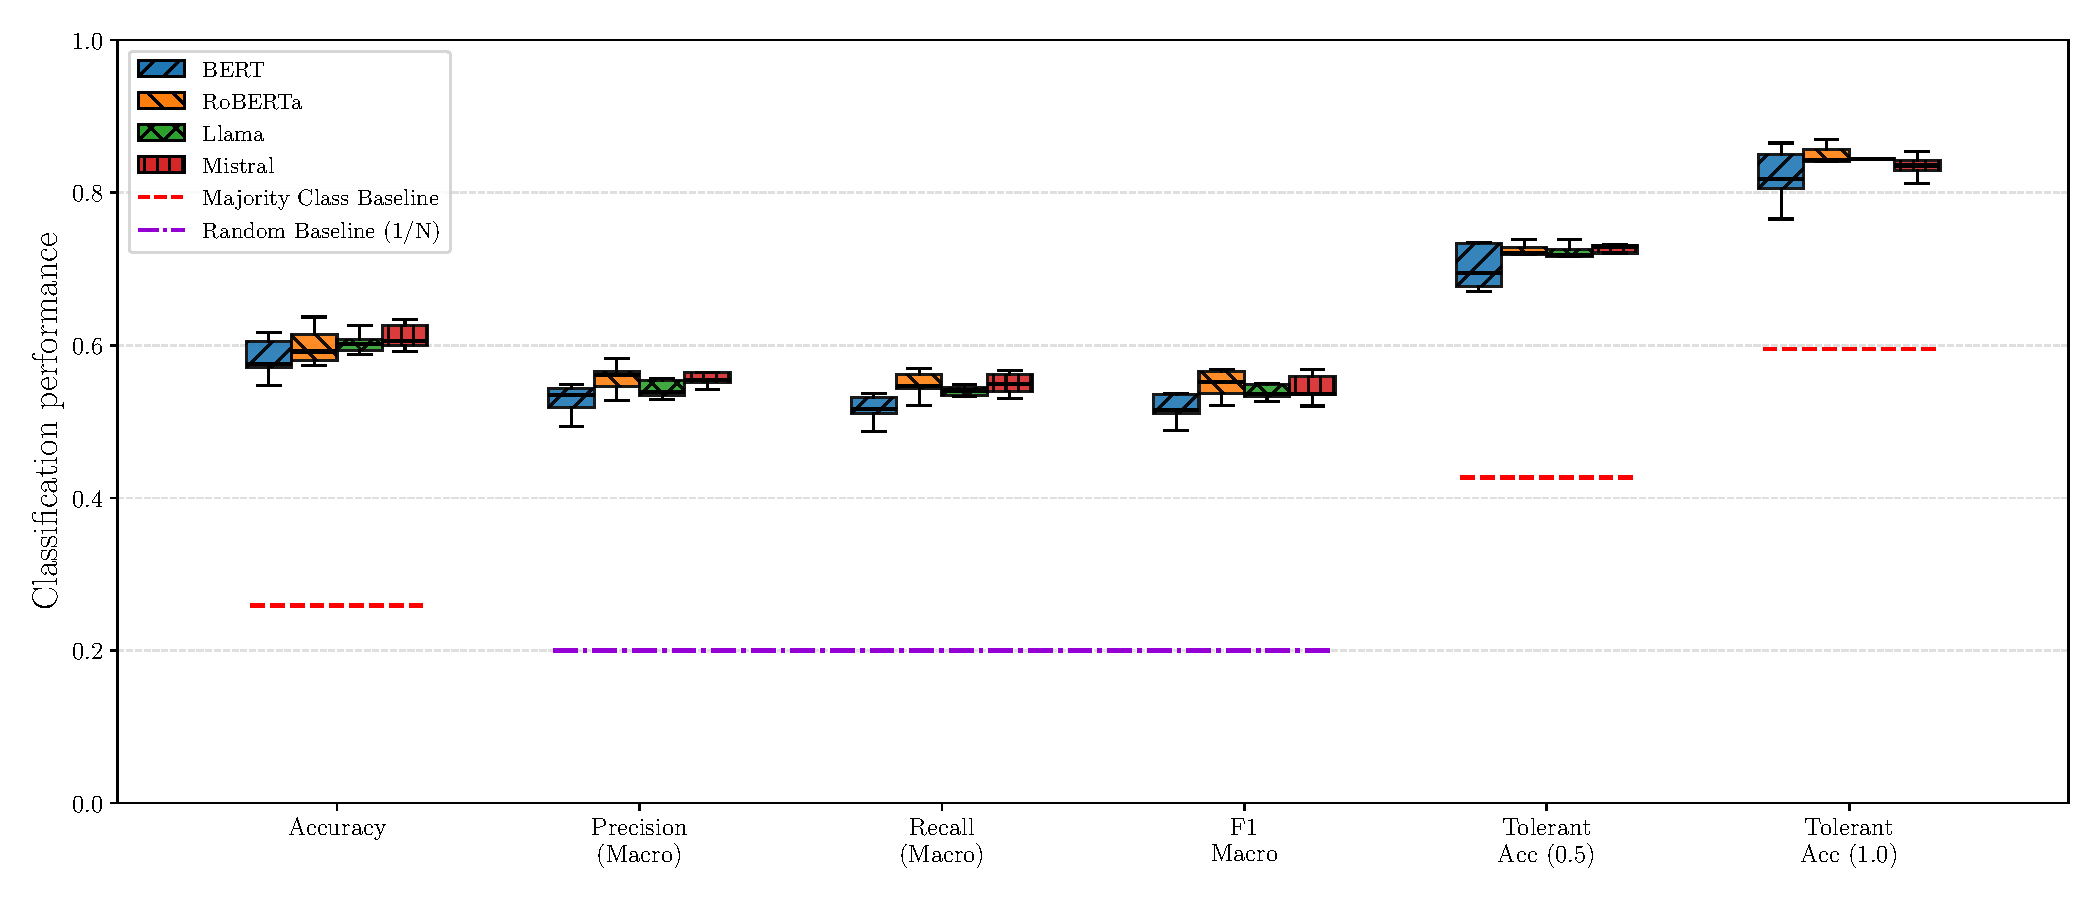
\includegraphics[width=1\columnwidth]{img/results_boxplot_baselines_updated.pdf}
    \caption{Distribution of evaluation metrics for BERT, RoBERTa, Llama, and Mistral across five folds. The boxplots report Accuracy, $\mathrm{Precision}_{\mathrm{macro}}$, $\mathrm{Recall}_{\mathrm{macro}}$, $\mathrm{F1}_{\mathrm{macro}}$, and two variants of $\mathrm{Accuracy}_{\mathrm{tolerant}}$ ($\alpha=0.5$ and $\alpha=1.0$). The horizontal lines represent the baselines: the dashed line is the Majority Class baseline (in red) and the dash-dotted line is the Random Baseline (in purple).}
\label{fig:results}
\end{figure}

Figure \ref{fig:results} illustrates the results. The dashed lines indicate the baselines. We distinguish between two references:
\begin{enumerate}
    \item \textbf{Majority Class Baseline (MCB)} (red): Used for Accuracy and Tolerant Accuracy. It represents a model that always predicts the most frequent label.
    \item \textbf{Random Baseline (RB)} (violet): Used for Macro metrics. Since macro-averaging treats all classes equally regardless of prevalence, the appropriate baseline is a uniform random guess ($1/N$).
\end{enumerate}
In terms of standard accuracy, all models achieve scores around 0.60, which is more than double the MCB. Mistral achieves the highest mean score of 0.61. Regarding macro-averaged performance, RoBERTa shows the highest mean $\mathrm{F1}_{\mathrm{macro}}$ of 0.55, followed by Mistral with 0.54. Llama and BERT rank just behind with 0.54 and 0.52, respectively. These scores significantly exceed the RB of 0.20. The variance across folds is minimal (standard deviation of approximately 0.02), indicating stability. The rightmost sections of the plot display tolerant accuracy. With a stricter penalty ($\alpha = 0.5$), Mistral, RoBERTa, and Llama reach approximately 0.72, which far exceeds the adjusted MCB of 0.43. 
When adjacent errors are considered fully correct ($\mathrm{Accuracy}_{\mathrm{tolerant}}$  = 1.0), RoBERTa achieves a top score of 0.84, followed by Mistral, Llama, and BERT with 0.83, 0.83, and 0.82, respectively. Although this metric's baseline is naturally higher (0.60), the models demonstrate significant performance gains (+0.24).
Results obtained for tolerant accuracy suggest that misclassifications are rarely severe, typically involving adjacent labels.

\subsection{Biases in Article-level reliability estimation}
\label{subsec:error_analysis}

Here, we study classification bias with respect to reliability level along two axes: (i) error frequency across levels, i.e., whether the classifier systematically performs better on some reliability classes than on others; and (ii) error direction, i.e., whether predictions tend to overestimate or underestimate the true reliability level.

\begin{figure}[h!]
    \centering
    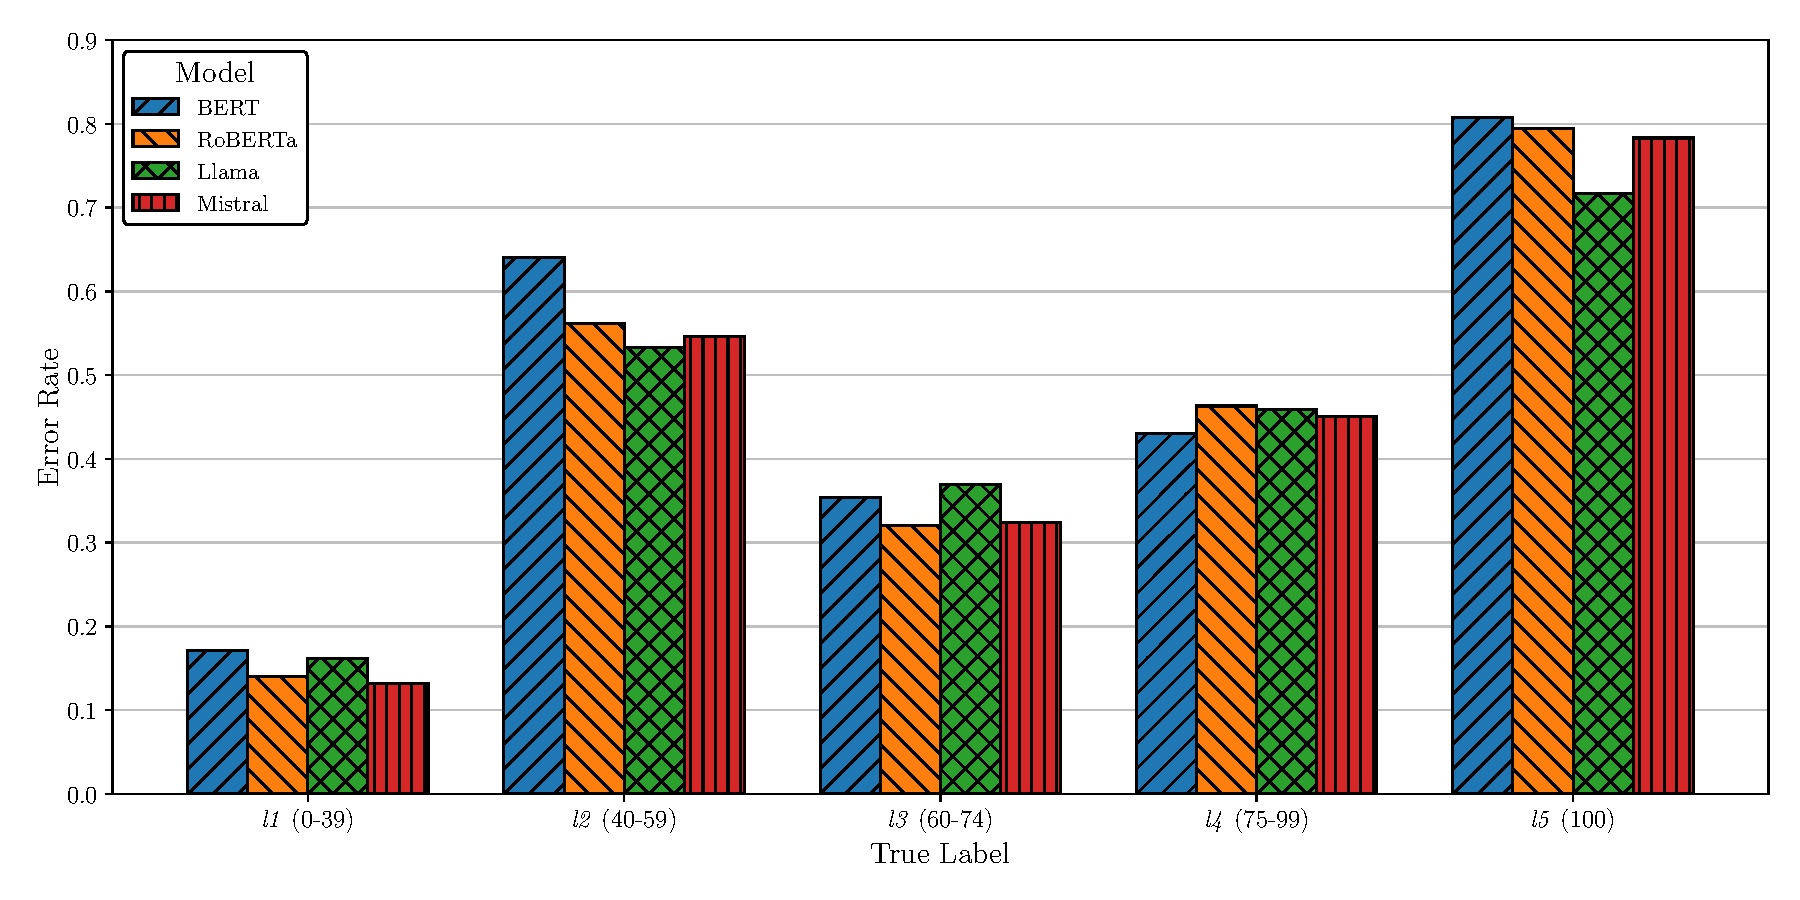
\includegraphics[width=1\columnwidth]{img/error_rate_analysis.pdf}
    \caption{Per-class error rate comparison. The error rate is defined as $(1 - \mathrm{Recall}_l)$, where $\mathrm{Recall}_l$ is the proportion of articles correctly assigned to level $l$ out of all articles truly belonging to that level.}
    \label{fig:error_rate}
\end{figure}

Figure~\ref{fig:error_rate} highlights an asymmetry in prediction correctness. The lowest error rates are on $l_1$ (error rate $< 0.20$). This suggests that highly unreliable content has recognizable structural features.
The highest-reliability articles ($l_5$) are the most challenging to recognize for the model, with error rates exceeding 70\%\footnote{We remind the reader that class $l_5$ only includes articles that have been given a reliability score of 100. It could easily be confused with $l_4$, which contains articles with similarly high scores. This could motivate the high error rate.}. Class $l_2$ also proves difficult, with an error rate of over 50\%. Class $l_3$ sits in the middle, showing a moderate error rate of approximately 35\% and performing significantly better than classes $l_2$ and $l_5$.

Figure \ref{fig:error_direction} plots the Mean Error Direction (MED) to quantify the prediction bias. MED is defined as the average signed difference between predicted and true reliability labels over misclassified instances (see Section~\ref{subsec:bias_methodology}). 
We observe a tendency to regress towards the center. We attribute this to two structural factors:

\begin{figure}[h!]
    \centering
    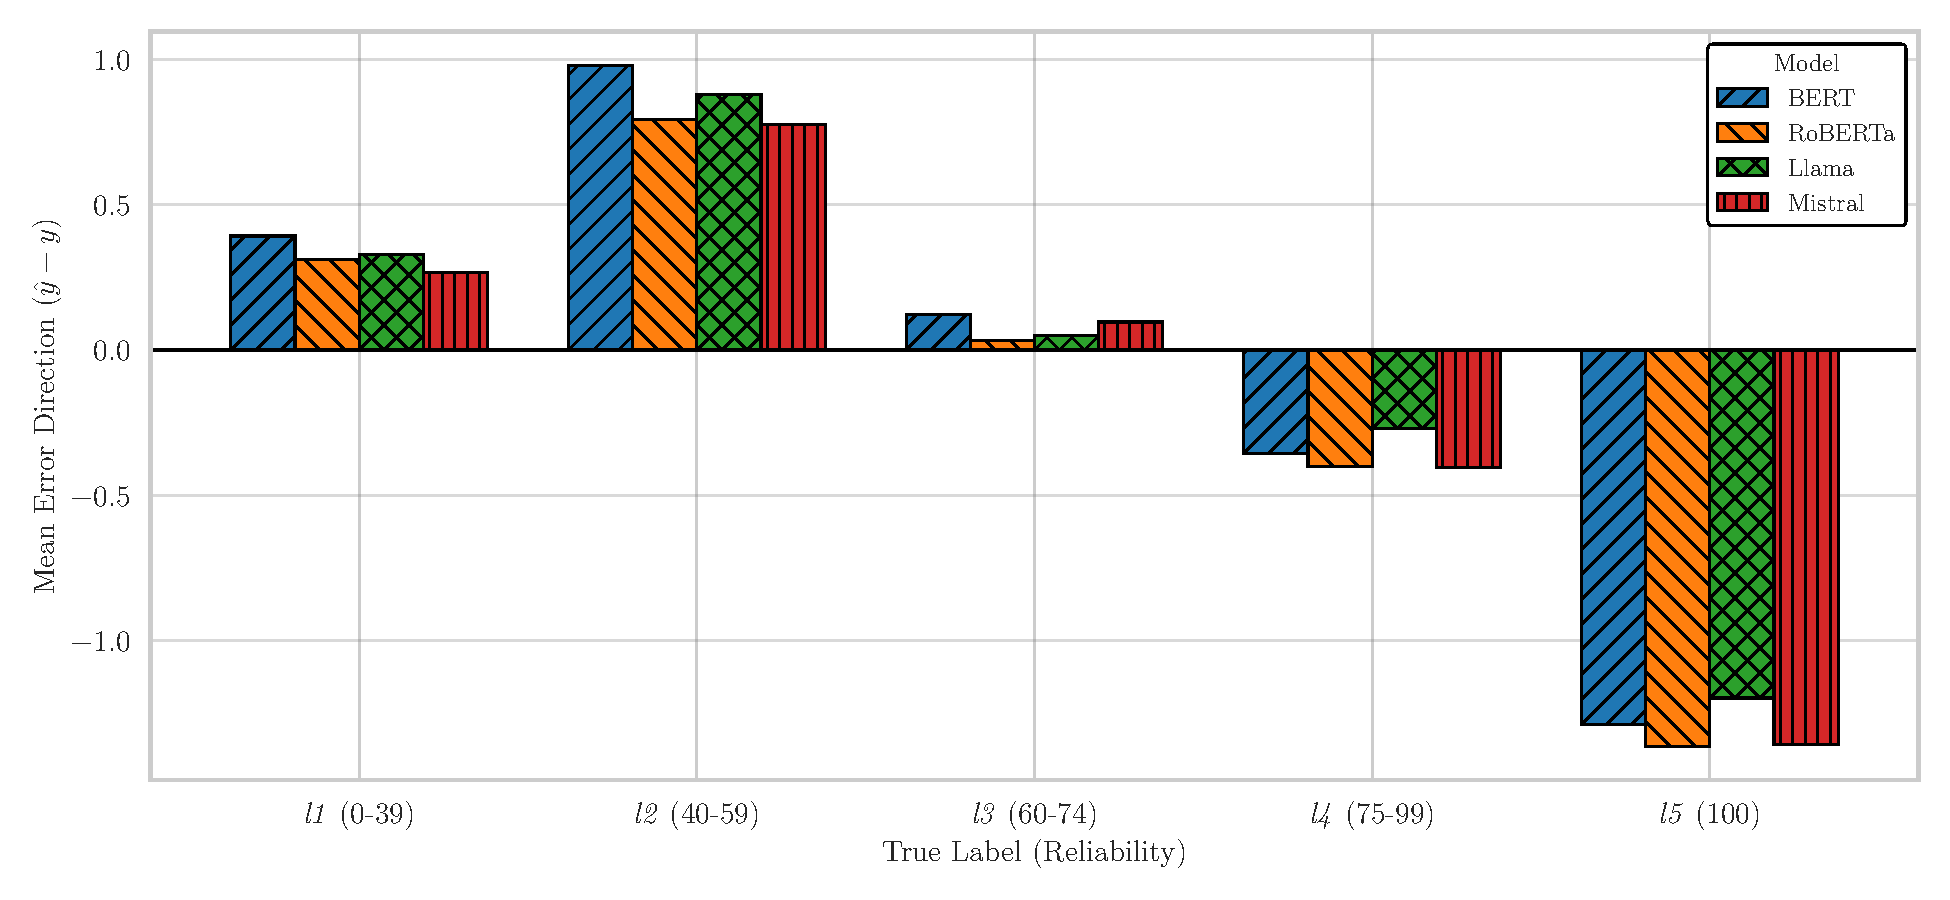
\includegraphics[width=1\columnwidth]{img/mean_error_direction.pdf}
    \caption{Mean Error Direction analysis. Positive values indicate overestimation of reliability, while negative values indicate underestimation.}    
    \label{fig:error_direction}
\end{figure}

\begin{itemize}
    \item \textbf{Boundary Constraints} ($l_1$ and $l_5$).
    Errors at the extremes are naturally constrained: models can only overestimate $l_1$ and underestimate $l_5$. However, the significant negative MED in $l_5$, $\approx -1.30 $ (BERT -1.29, RoBERTa -1.37, Llama -1.20, Mistral -1.36). The confusion matrices reveal that the vast majority of misclassifications for $l_5$ are concentrated in adjacent $l_4$ \cite{bianchi2026supplementary}. This confirms that the high error rate is primarily due to the models struggling to distinguish between perfect (100) and generally credible (75–99) reliability, likely because there is little textual distinction between these high-standard categories. The fact that the MED is slightly below -1.0 indicates a minor tendency to misclassify some $l_5$ instances into lower tiers (levels 2 and 3), but the main misclassification consists of labeling $l_5$  as $l_4$ . 
    
    \item \textbf{The `Safe Harbor' Effect ($l_3$).} 
    Class $l_3$ shows a Mean Error Direction close to zero (0.03 to 0.12 across models, with Mistral at 0.10). $l_3$ acts as a gravitational center for uncertainty: it absorbs a significant portion of misclassifications from the lower-reliability $l_2$ and from the higher-reliability $l_4$. Since the model overestimates $l_2$ (pushing it up to 3) and underestimates $l_4$ (pushing it down to 3), these opposing error vectors cancel each other out, resulting in a net directional bias of zero.    
\end{itemize}

These directional patterns generally remain consistent across all four models, including the substantially larger Mistral, suggesting that the biases are structural properties of the task rather than intrinsic to a specific architecture or model scale; the Supplementary Material~\cite{bianchi2026supplementary} reports full confusion matrices across all five cross-validation folds.

\subsection{Influence of Political Leaning on Classification Errors}\label{subsec:politicalBias}
% -------------------------------------------------------------------------
\begin{figure}[h!]
    \centering
    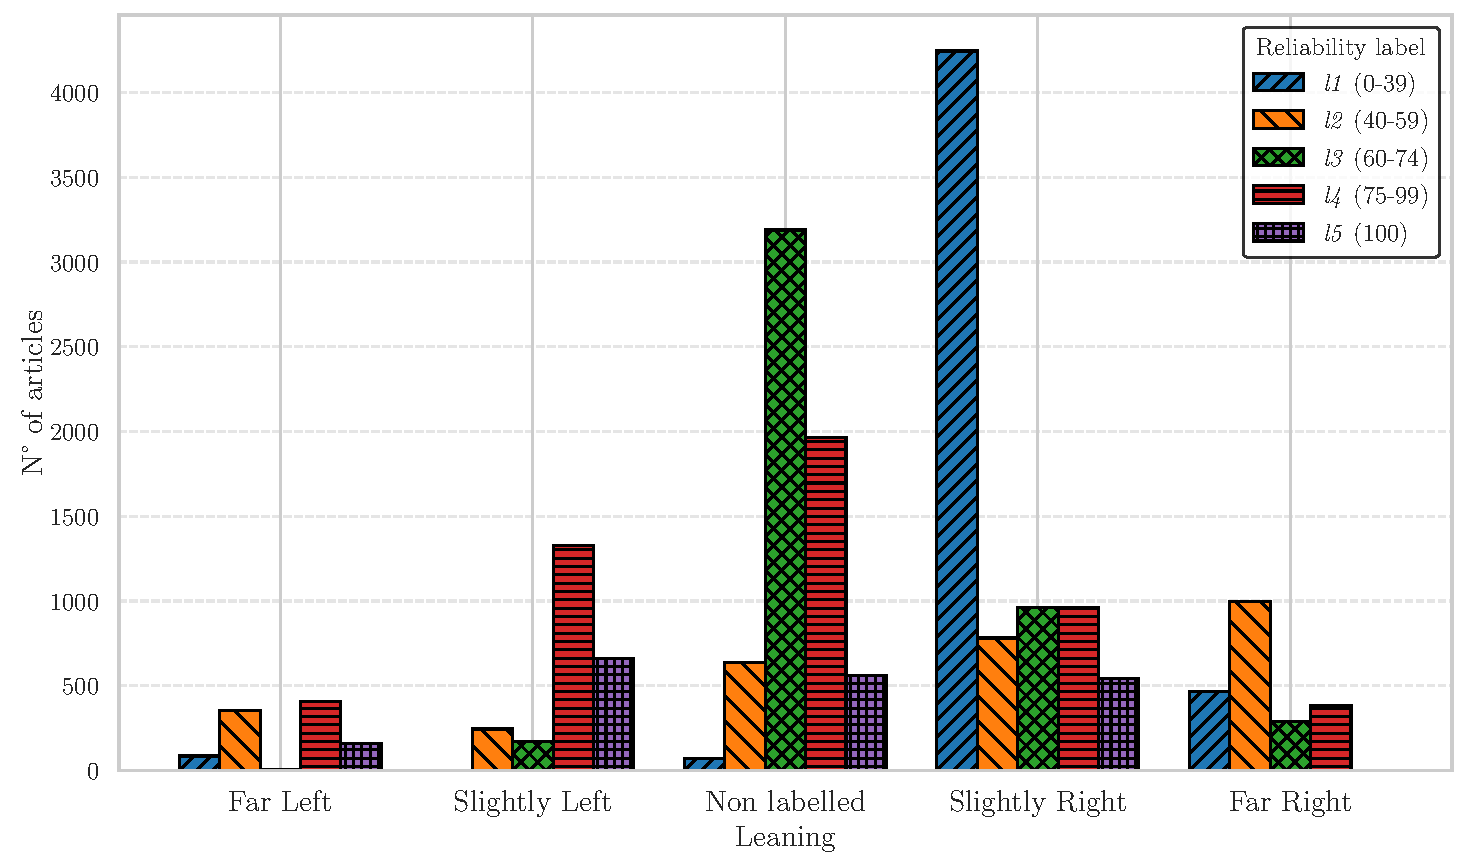
\includegraphics[width=\columnwidth]{img/orientationDistributionInverted.pdf}
    \caption{Distribution of reliability labels across political leanings. Each color and hatch pattern represents a distinct reliability level. Non labelled indicates articles from publishers not categorized by NewsGuard with respect to political leaning.}
    \label{fig:orientationDistributionInverted}
\end{figure}

The core objective of this section is to determine if the models exhibit political bias. Specifically, we investigate whether the models treat all sides of the political spectrum equally or if they penalize specific orientations.

We recall that, in the present study, the political orientation is a property of the publisher (i.e., the domain), not of the individual article.
Since the classifiers operate at the article level, the publisher’s political leaning is inherited by each article it produces, i.e., \(o_A(a) = o_P(p(a))\) (see Section \ref{subsec:problemdef}). This enables a post-hoc analysis of how source-level political alignment relates to article-level prediction errors.
Aimed at revealing whether the models behave uniformly across the political spectrum or whether notable political patterns emerge, this analysis proceeds in three steps:

\begin{enumerate}
    \item \textbf{Distribution Analysis.} First, we map how political orientations are distributed across reliability classes in our dataset (Figure \ref{fig:orientationDistributionInverted}).

    \item \textbf{Error Rate Analysis.} Second, we provide a quantitative assessment of the errors made by the models with respect to political orientation. Specifically, we evaluate whether misclassification errors are unevenly distributed across political leanings (Figure~\ref{fig:politicalErrorRates}) and test the statistical significance of these differences (Table~\ref{tab:chi_square_results}).

    \item \textbf{Directional Bias Analysis.} Finally, we quantitatively assess whether, among misclassified instances, the models exhibit systematic directional biases—specifically, a tendency to overestimate reliability (positive bias) or to underestimate it (negative bias)—as a function of political leaning (Figure~\ref{fig:politicalErrorsDirection}).
\end{enumerate}

\begin{table}[t]
\centering
\begin{tabular}{lcccc}
\textbf{Model} & \textbf{Accuracy} & $\boldsymbol{\chi^2}$ & \textbf{$p$-value} & \textbf{Cramér’s V} \\
\midrule
BERT & 58.27\% & 1684.13 & $<10^{-300}$ & 0.294 \\
RoBERTa & 60.34\% & 1418.31 & $<10^{-300}$ & 0.270 \\
Llama & 59.97\% & 1207.83 & $<10^{-250}$ & 0.249 \\
Mistral & 61.16\% & 1343.98 & $<10^{-300}$ & {0.263} \\
\end{tabular}
\caption{
Statistical tests for Political Leaning vs. Classification Correctness. The table reports the Chi-square ($\chi^2$) test of independence and the associated $p$-values to assess whether error rates vary across political orientations. Cramér’s V is provided to measure the effect size of this association.}
\label{tab:chi_square_results}
\end{table}

Figure~\ref{fig:orientationDistributionInverted} shows an imbalance across political orientations in the dataset. Accordingly, we compute error rates separately for each leaning, defined as the proportion of misclassified instances within each class. This class-conditional formulation makes error rates independent of class frequency, allowing us to analyze model errors despite the overall imbalance.


The resulting mean misclassification rates computed for each model and political orientation are reported in Figure~\ref{fig:politicalErrorRates}. We observe that all models exhibit systematic variation in performance across political leanings. There are substantially higher error rates for far left and far right outlets (59–72\%) compared to lower rates for slightly right and non-labeled outlets (30–34\%), and intermediate error rates for slightly left articles (47–58\%).  Mistral 24B deviates from the other models by showing fewer errors in the extreme categories and a higher error rate in the Slightly Left category. Its performance is comparable in the Non-labelled and Slightly Right categories.


To assess the statistical significance of the observed bias, we apply a chi-square test of independence. The null hypothesis assumes that classification correctness is independent of political leaning. For all models, this hypothesis is rejected (Table~\ref{tab:chi_square_results}), indicating that misclassification rates are significantly associated with political orientation. Cramér’s~$V$ further reveals a consistent small-to-moderate effect size.

\begin{figure}[t]
    \centering
    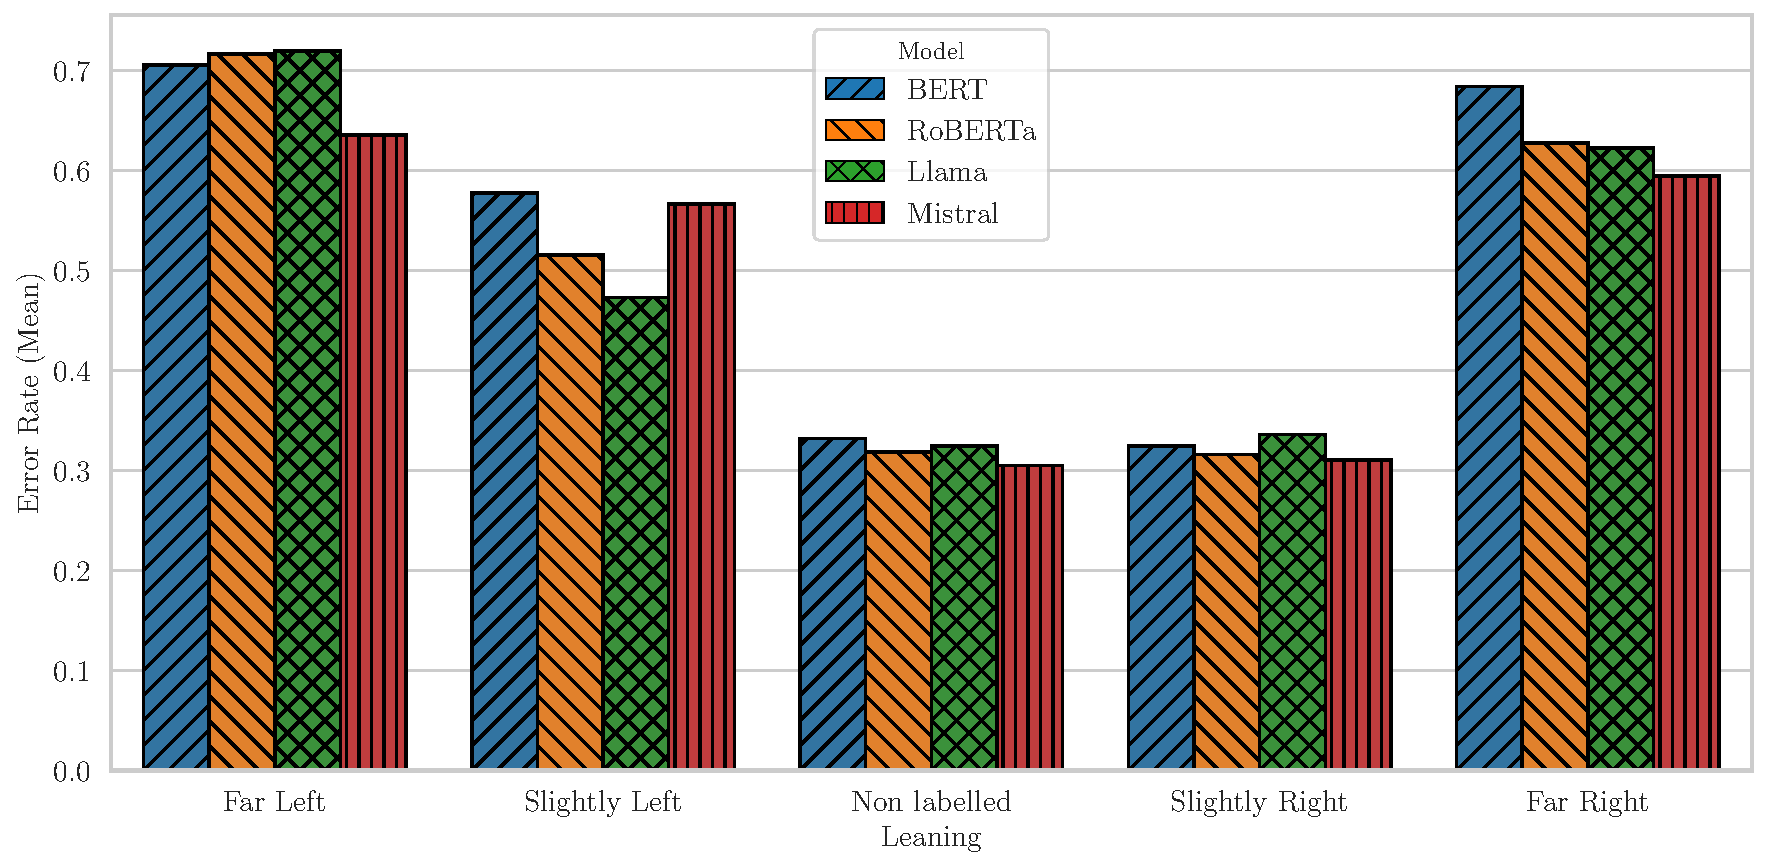
\includegraphics[width=\columnwidth]{img/politicalErrorRates.pdf}
    \caption {Error rate by political orientation and model. The bar chart displays the proportion of incorrect predictions for each model across the five political leanings. The error rate is calculated as the ratio of incorrect predictions to the total number of predictions (equivalent to the mean of a binary variable where 1 = incorrect and 0 = correct).}
    \label{fig:politicalErrorRates}
\end{figure}

As a third analysis, we focus on misclassified instances to assess whether models exhibit directional biases, namely systematic tendencies to overestimate or underestimate article reliability as a function of political leaning. Figure~\ref{fig:politicalErrorsDirection} reports the Mean Error Direction (MED), defined as the average signed difference between predicted and true reliability labels over misclassified instances for each orientation (see Section~\ref{subsec:bias_methodology}). As anticipated in Section \ref{subsec:error_analysis}, positive MED values indicate overestimation of reliability, whereas negative values indicate underestimation.

Clear directional patterns emerge across all four models. Far Left and Far Right articles exhibit consistent overestimation, with mean signed errors ranging from +0.33 to +1.00, approaching a full reliability level. Slightly Left articles show systematic underestimation, with average values between -0.54 and –0.82. Slightly Right and non-labeled outlets display smaller, less consistent deviations: Llama, RoBERTa, and Mistral slightly underestimate Slightly Right reliability (up to -0.39), whereas BERT slightly overestimates it; for non-labeled outlets, BERT, Llama, and Mistral exhibit mild positive biases, while RoBERTa's average bias is near zero; the Supplementary Material~\cite{bianchi2026supplementary} reports full confusion matrices stratified by political leaning.

\begin{figure}[t!]
    \centering
    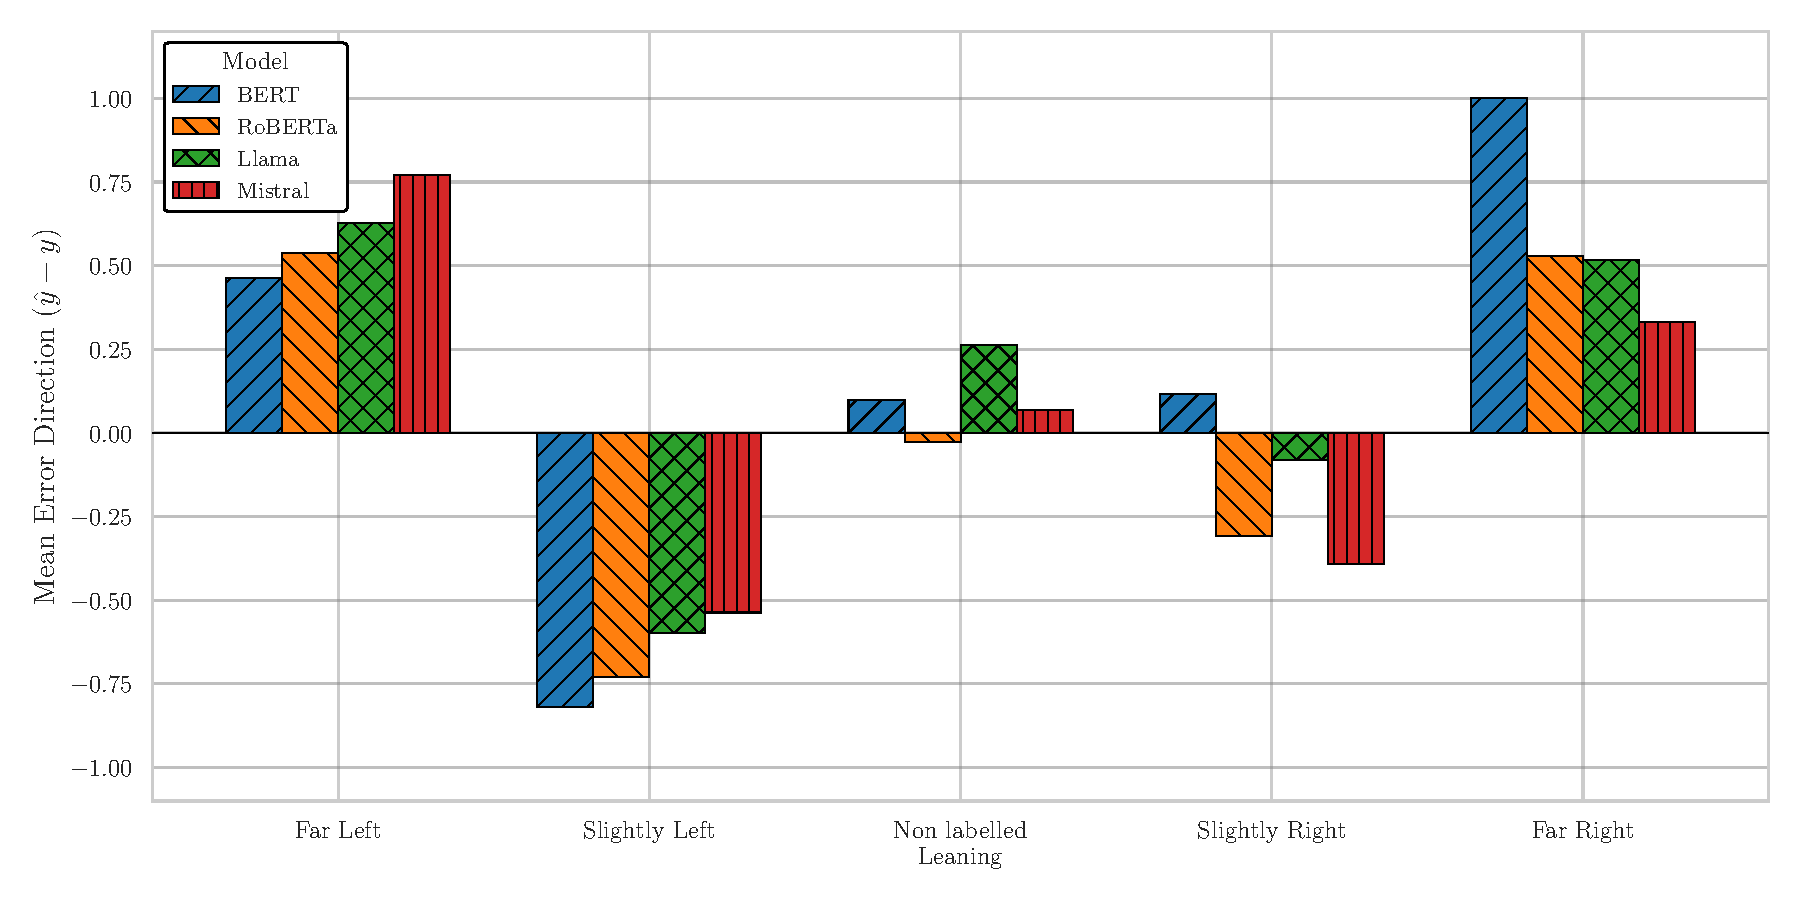
\includegraphics[width=\columnwidth]{img/politicalErrorsDirection.pdf}
    \caption{Mean value and direction of misclassifications, stratified by political leaning. Positive values indicate overestimation (prediction $>$ true label), while negative values indicate underestimation.}
    \label{fig:politicalErrorsDirection}
\end{figure}


\subsection{Stage 2: Publisher reliability inference}

The publisher-level inference task constitutes the primary objective of this work. The article-level estimators analyzed in the previous section are not the final target of the framework, but rather intermediate components used to infer the reliability of previously unseen news sources.

As anticipated in Section~\ref{sec:problemDef}, publisher-level reliability is obtained by aggregating article-level predictions for each publisher. To evaluate this approach, we use a simple aggregation function, \(Agg\), which is defined as the mode of a publisher’s article-level predictions (i.e., majority voting).
For a given publisher \(p \in P\), the system collects the predicted reliability labels \(C_{\text{reliability}}(a)\) for all articles \(a \in A_p\) in the test set (the predicted labels for the articles in each of the five test folds) and assigns the most frequent class as the final publisher-level label \(\hat{r}_P(p)\).
For example, if a publisher has ten articles and six are classified as \(l_4\) while four are classified as \(l_3\), the resulting publisher-level label is \(l_4\). This aggregation strategy is based on the hypothesis that combining predictions from multiple articles can offset the impact of variability or noise in individual classifications.

Our analysis considers all article-level predictions across the test sets, thereby simulating an \emph{in-the-wild} deployment scenario. In this scenario, the reliability of the publisher is inferred exclusively from the articles in the test set, ensuring that the model estimates the reliability of a source without having observed any of its content during training.


\begin{figure}[t]
  \centering
  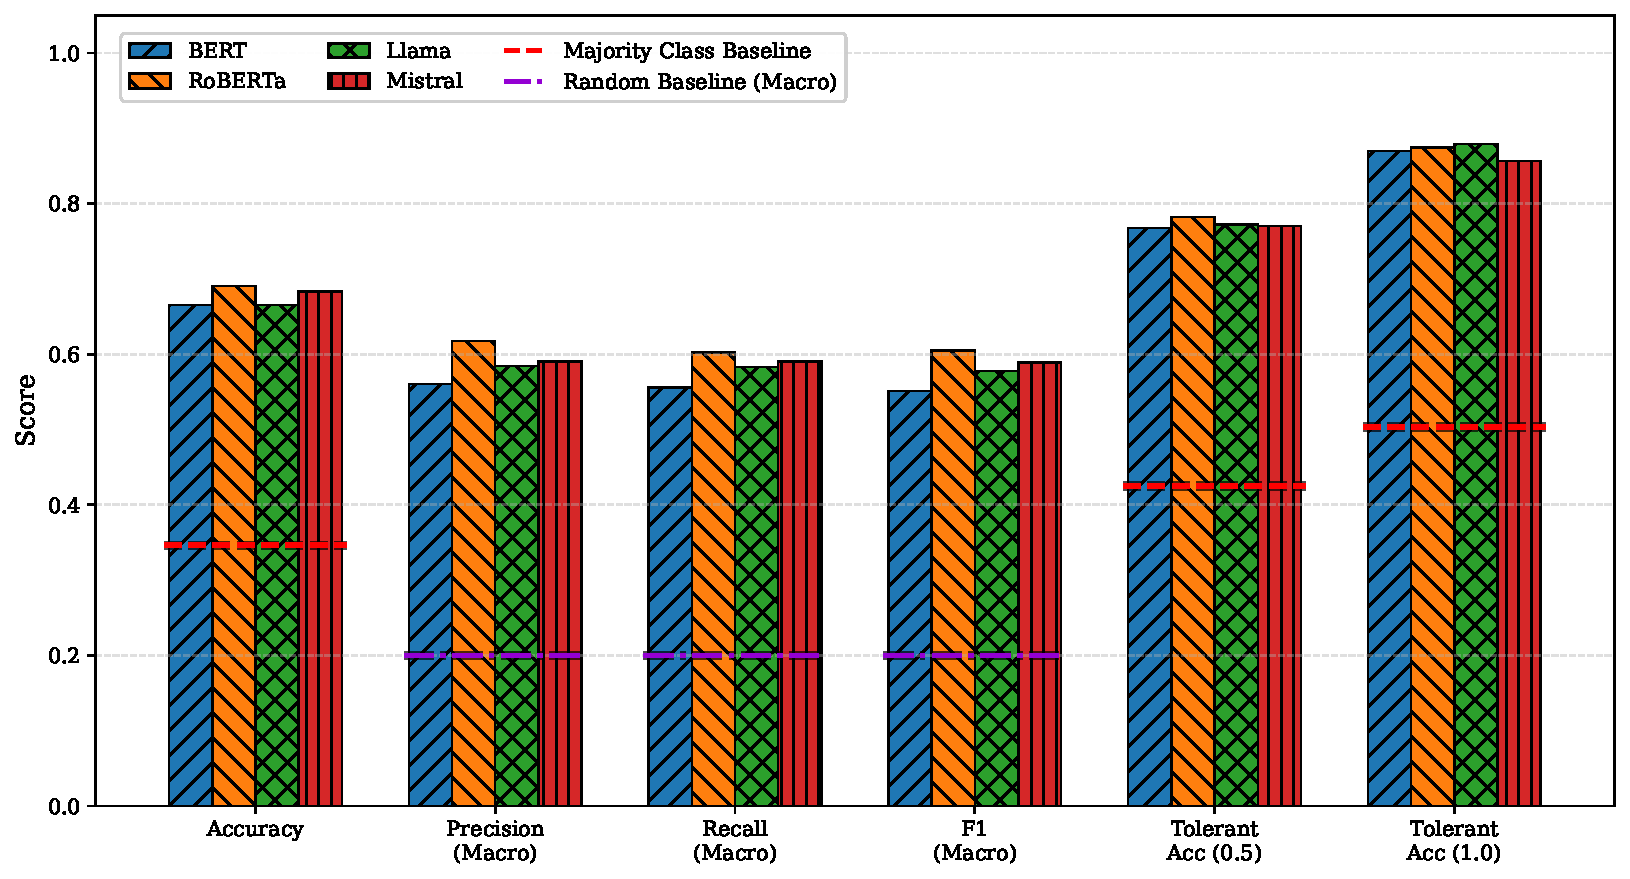
\includegraphics[width=\columnwidth]{img/domain_metrics_comparison.pdf}
  \caption{Publisher reliability prediction: performance metrics for BERT, RoBERTa, Llama, and Mistral. Dashed red lines indicate the Majority Class Baseline (for Accuracy and Tolerant Accuracy); dash-dotted violet lines indicate the Random Baseline at 0.20 (for Macro metrics).}
  \label{fig:metrics}
\end{figure}

Figure \ref{fig:metrics} presents the results. The bar chart benchmarks performance against two distinct baselines, represented by dashed lines:
\begin{itemize}
    \item \textbf{Majority Class Baseline (MCB) (Red):} Represents a model that always predicts the most frequent domain label. It serves as the reference for Accuracy and Tolerant metrics. Note that the three red lines differ: for example, a majority predictor achieves a given Accuracy by always predicting $l_4$, but under Tolerant Accuracy (0.5) it also receives half credit for $l_3$ and $l_5$ predictions that fall one step away, and full credit under Tolerant Accuracy (1.0), progressively raising the baseline value across the three metrics.
    \item \textbf{Random Baseline (RB) (Violet, 0.20):} Represents a uniform random guess ($1/N$). This is the reference for Macro metrics, as they weight all classes equally regardless of their size.

\end{itemize}

With an Accuracy of 0.69 RoBERTa leads, followed closely by Mistral at 0.68. These scores are more than triple those of the Random Baseline. 
Considering $\mathrm{Accuracy}_{\mathrm{tolerant}}$  (1.0), Llama achieves the top score of 0.88, followed by RoBERTa (0.87) and Mistral (0.86). These scores substantially outperform the majority class baseline.

Publisher-level errors are strictly local and concentrate between adjacent reliability levels, most notably between $l_4$ (Generally Credible) and $l_5$ (High Credibility); the Supplementary Material~\cite{bianchi2026supplementary} reports full publisher-level confusion matrices and a detailed error analysis.


%VECCHIA VERSIONE
%The confusion matrices reveal that errors are strictly local. The most frequent confusion occurs between $l_4$ (Generally Credible) and $l_5$ (High Credibility). As was previously observed in the article-level predictions, it is inherently difficult to distinguish between $l_4$ and $l_5$ because $l_5$ acts as a strict ceiling and $l_4$ covers the immediate high range. However, misclassifying these two labels constitutes a minor severity error since both indicate high reliability.




% \textcolor{blue}{IO LA CHIUDEREI QUI per questo articolo. 
%Il restante lo mettiamo nel tool. }
%\{However, a practical constraint in automated source analysis is resource efficiency. Must we analyze hundreds of articles to characterize a domain, or is a small snapshot sufficient? To answer this, we performed a \textit{Randomized Block Analysis} to simulate real-world scenarios where data access is limited.}

%\{The experimental protocol proceeds as follows for each unique domain in the dataset:}
%\begin{itemize}
%    \item \{\textbf{Pooling \& Shuffling:} We aggregate all available article-level predictions for the domain and randomize their order. This step removes temporal correlations and simulates a random sampling process.}
%    \item \{\textbf{Block Partitioning:} We divide the shuffled predictions into non-overlapping "chunks" of size $N$, with $N$ ranging from 5 to 100 articles. Any remainder insufficient to fill a block is discarded.}
%    \item \{\textbf{Aggregation \& Evaluation:} For each chunk, we assign a domain label via majority voting (mode of the article predictions). The chunk itself is then treated as a single prediction instance and compared against the ground truth domain label.}
%\end{itemize}
%\{This approach allows us to measure classification performance as a function of sample size ($N$). It is important to note that as $N$ increases, the total number of available chunks (visualized by the grey bars in Figure \ref{fig:DomainSizeComparision}) decreases, as domains with fewer than $N$ articles are naturally excluded from the analysis.}

%\begin{figure}[htbp]
%    \centering
    % --- Prima Figura: BERT ---
%     \begin{subfigure}[b]{0.48\textwidth}
%         \centering
%         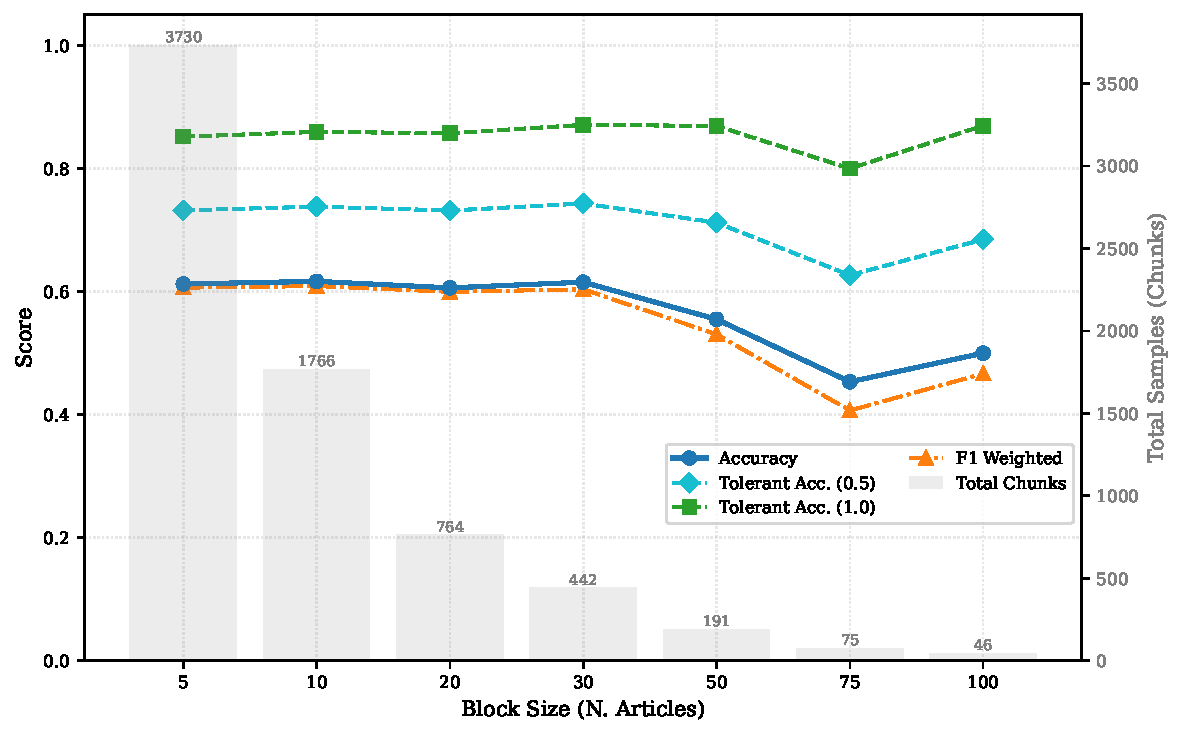
\includegraphics[width=\linewidth]{img/analysis_bert_enriched_mode.pdf}
%         \caption{BERT}
%         \label{fig:bert}
%     \end{subfigure}
%     \hfill 
%     % --- Seconda Figura: RoBERTa ---
%     \begin{subfigure}[b]{0.48\textwidth}
%         \centering
%         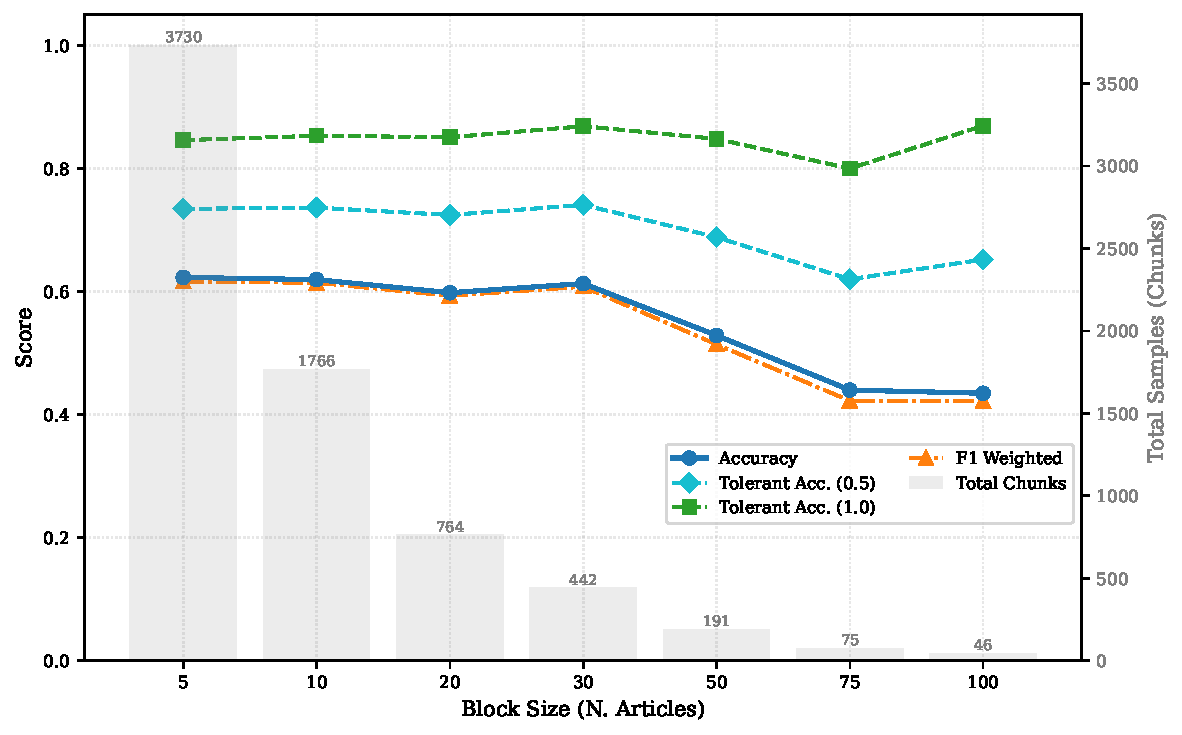
\includegraphics[width=\linewidth]{img/analysis_roberta_enriched_mode.pdf}
%         \caption{RoBERTa}
%         \label{fig:roberta}
%     \end{subfigure}
%     \hfill 
%     % --- Terza Figura: Llama ---
%     \begin{subfigure}[b]{0.48\textwidth}
%         \centering
%         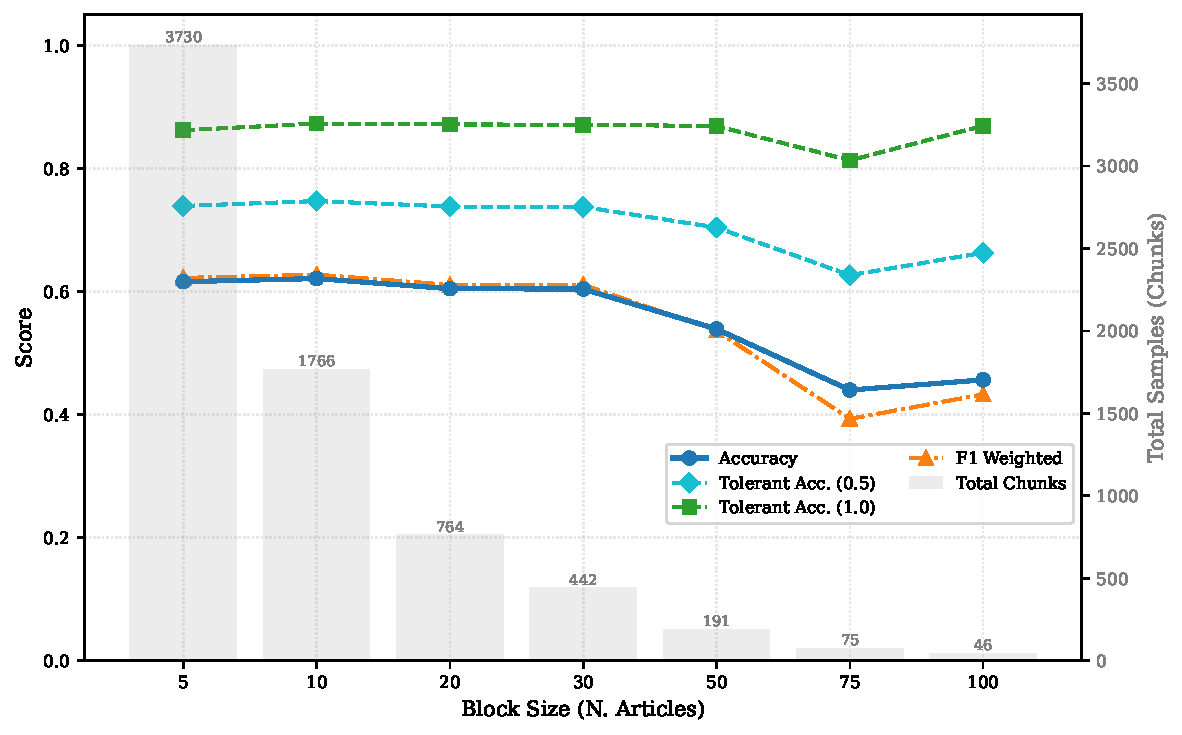
\includegraphics[width=\linewidth]{img/analysis_llama_enriched_mode.pdf}
%         \caption{Llama}
%         \label{fig:llama}
%     \end{subfigure}
    
%     \caption{Impact of aggregation size ($N$) on domain classification. The curves track performance metrics when the domain label is predicted via majority voting on a random block of $N$ articles. The grey bars (secondary axis) represent the total number of evaluation chunks available, which naturally decreases as larger block sizes exclude domains with insufficient articles.}    \label{fig:DomainSizeComparision}
% \end{figure}
% \{Figure \ref{fig:DomainSizeComparision} presents the results of this simulation. Contrary to the expectation that "more is better," performance peaks with small sample sizes ($N=5$ to $10$). At just 10 articles, Llama3 and RoBERTa achieve their optimal exact accuracy (~0.62) and high stability (Tolerant Accuracy $\approx$ 0.87). 
% As $N$ increases to 50 or 100, exact accuracy paradoxically declines. This trend likely reflects the composition of the test set rather than model failure: only a small subset of specific domains possesses enough articles to form large blocks (46 chunks at $N=100$ vs. 3730 at $N=5$), and these domains appear inherently more ambiguous. Nevertheless, the Tolerant Accuracy remains robust (>0.80) even at large sizes for all models. 
% Crucially, this finding implies that scraping just 5 to 10 articles is sufficient to profile a source with state-of-the-art reliability, optimizing computational resources for large-scale monitoring.}

% \section{Political leaning}

% In questa sezione analizziamo i casi di errore per valutare l’influenza del political leaning sulle decisioni del modello in materia di affidabilità. Gli esperimenti mirano a determinare se gli errori siano bilanciati rispetto al political leaning, sia in termini di frequenza sia di direzione, ossia se il modello tenda a penalizzare o favorire sistematicamente l’affidabilità in funzione dell’orientamento politico.

% \begin{itemize}
%     \item Fig. \ref{fig:orientationDistribution} 
%     \item Si osserva che  che gli errori commessi non sono bilanciati in modo statisticamente significativo rispetto al political learning. Infatti, la Fig. \ref{fig:politicalErrorRates} mostra etcetc. A supporto, la Tabella \ref{tab:chi_square_results} indica che a prescindere dallo sbilanciamneto ooservato precedentemente lo sbilanciamento è statisticamente significativo per tutti i modelli (statistiche).
%     \item Dalla Fig. \ref{fig:politicalErrorsDirection} si evidenziano pattern sistematici in cui il modello, a seconda del leaning, tende a sovrastimare gli articoli di certi political leaning. Commenta confronto Nautral vs. political (neutral non gli da direzione mentre political si); differenza slightly left / right; differenza slightl con far.  
%     \item (in discussion) Il nostro modello ha dei bias da mitigare in sviluppi successivi (in linea con quell che esiste?)

% \end{itemize}


% \section{Reliability labels and political leanings } The reliability labels assigned by NewsGuard correlate with a variety of editorial and stylistic practices which, in turn, may interact with the political orientation of news outlets. Understanding whether such interactions affect model behavior is important both for interpreting performance and for identifying potential sources of systematic error. In this section, we examine whether the political leaning of a publisher is associated with higher misclassification rates or with consistent directional biases in the predicted reliability levels.

% Our analysis proceeds in three steps. First, we describe the distribution of political orientations across reliability labels, to contextualize the dataset and potential confounding factors (Figure \ref{fig:orientationDistribution}). Second, we assess whether error rates differ across political orientations, and whether these differences are statistically significant (Figure \ref{fig:politicalErrorRates}). Finally, we examine the direction of misclassifications, asking whether the models tend to systematically overestimate or underestimate reliability depending on political leaning (Figure \ref{fig:politicalErrorsDirection}). Together, these experiments allow us to evaluate whether models behave uniformly across political groups or whether notable patterns emerge.

% The information about the political leaning of the news outlet is also taken from NewsGuard. As for the reliability
% score, we transfer the political label assigned to the news outlet to the individual news items from that outlet. Thus,
% with a slight abuse of notation, we discuss articles that are far left, slightly left, and so on, when in reality they
% originate from news outlets labeled accordingly. For the analysis, we aggregate the predictions generated across the five
% test folds of the stratified cross-validation procedure described above. This allows us to evaluate the entire dataset and
% also without bias, as each prediction was produced by a model that had not been trained on the corresponding sample. 

% \subsection{Distribution of political orientations across reliability levels}

% Figure \ref{fig:orientationDistribution} reports how the political orientation of news outlets is distributed across the five reliability labels. Several imbalances arise: Label 1 is dominated by “Slightly Right” outlets, Label 2 is primarily composed of “Far Right” and “Slightly Right” sources, and Labels 3–4 contain large fractions of non-labelled outlets. Label 5 is comparatively small but more balanced, including “Slightly Left”, non-labelled, and “Slightly Right” outlets. These patterns highlight that political orientation and reliability are not independent in the underlying media ecosystem, motivating a careful examination of how models behave across groups.

% \subsection{Error rates across political orientations}
% We next analyze whether models make more errors for articles from certain political orientations. Figure \ref{fig:politicalErrorRates} shows the mean misclassification rate for each model and orientation, where 0 denotes a correct prediction and 1 an error. All models exhibit substantially higher error rates for articles from “Far Left” and “Far Right” outlets, with values ranging from 62\% to 72\%, compared to substantially lower rates for “Slightly Right” and non-labelled outlets (31–33\%) and intermediate rates for “Slightly Left” articles (47–58\%).

% Importantly, these differences cannot be explained solely by sample size effects. For instance, although the “Slightly Left” category is comparable in size to “Far Right”, its error rates are notably lower. To formally assess whether error rates depend on political orientation, we apply a chi-square test of independence between political leaning and classification correctness (see Section 3.2). For all models, the null hypothesis of independence is decisively rejected (Table \ref{tab:chi_square_results}), indicating that misclassification frequency is not uniformly distributed across political orientations. Cramer's V further confirms a small-to-moderate but consistent association between leaning and error behavior.

% \subsection{Direction of misclassifications}
% Error frequency alone does not reveal whether models systematically overestimate or underestimate reliability for certain orientations. To investigate this, we compute the mean signed error (predicted label minus true label), aggregated by political leaning (Figure \ref{fig:politicalErrorsDirection}). Positive values indicate overestimation; negative values indicate underestimation.

% Clear directional patterns emerge across all three models.

% Far Left and Far Right articles exhibit consistent overestimation, with mean signed errors ranging from +0.46 to +1.00, approaching a full reliability level.

% Slightly Left articles show systematic underestimation, with average values between –0.60 and –0.82.

% Slightly Right and non-labelled outlets display smaller, less consistent deviations: Llama and RoBERTa slightly underestimate “Slightly Right” reliability, whereas BERT slightly overestimates it; for non-labelled outlets, BERT and Llama exhibit mild positive biases while RoBERTa's average bias is near zero.

% These results indicate that models do not only differ in error frequency across political orientations but also in error direction, suggesting that some political groups are systematically pushed toward higher or lower predicted reliability levels.

% \subsection{Identifying the orientations driving dependence}

% To better understand which political orientations contribute most to the statistical dependence identified by the chi-square test, we examine the cell-wise contributions to the chi-square statistic (Section 3.2). This analysis confirms that the largest deviations from expected values occur for “Far Left” and “Far Right” orientations, which contribute disproportionately to the overall test statistic. These findings underscore that extreme political orientations are the primary drivers of the observed dependence between political leaning and classification correctness.


% \section{Political leaning}


% \begin{figure}[h!]
%     \centering
%     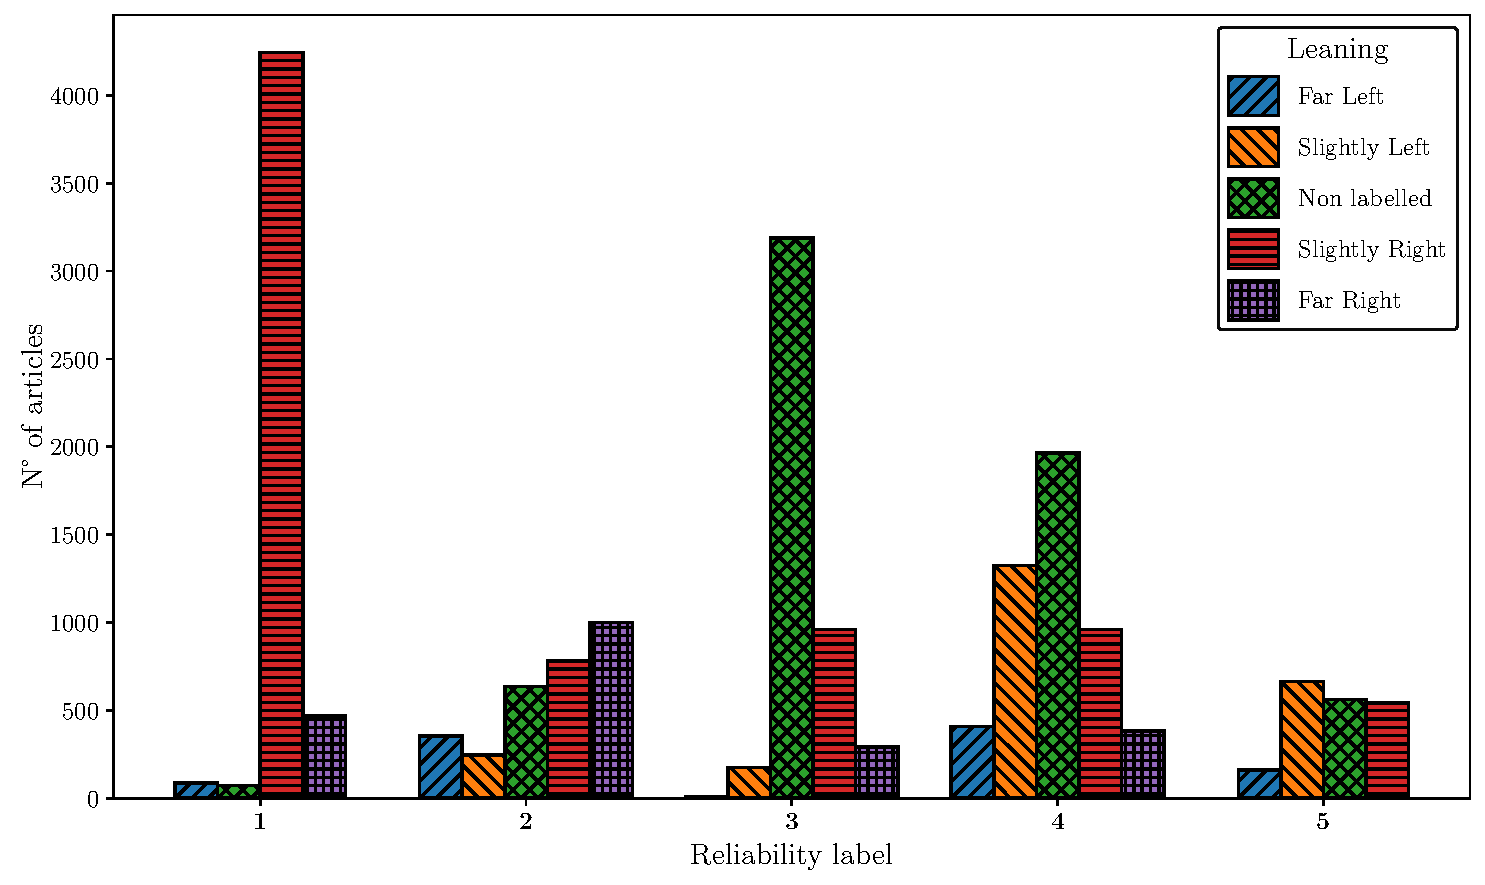
\includegraphics[width=1\columnwidth]{img/orientationDistribution.pdf}
%     \caption{Distribution of political leanings across reliability labels. Each color and hatch pattern represents a distinct political leaning category.}
%     \label{fig:orientationDistribution}
% \end{figure}


% \begin{figure}[h!]
%     \centering
%     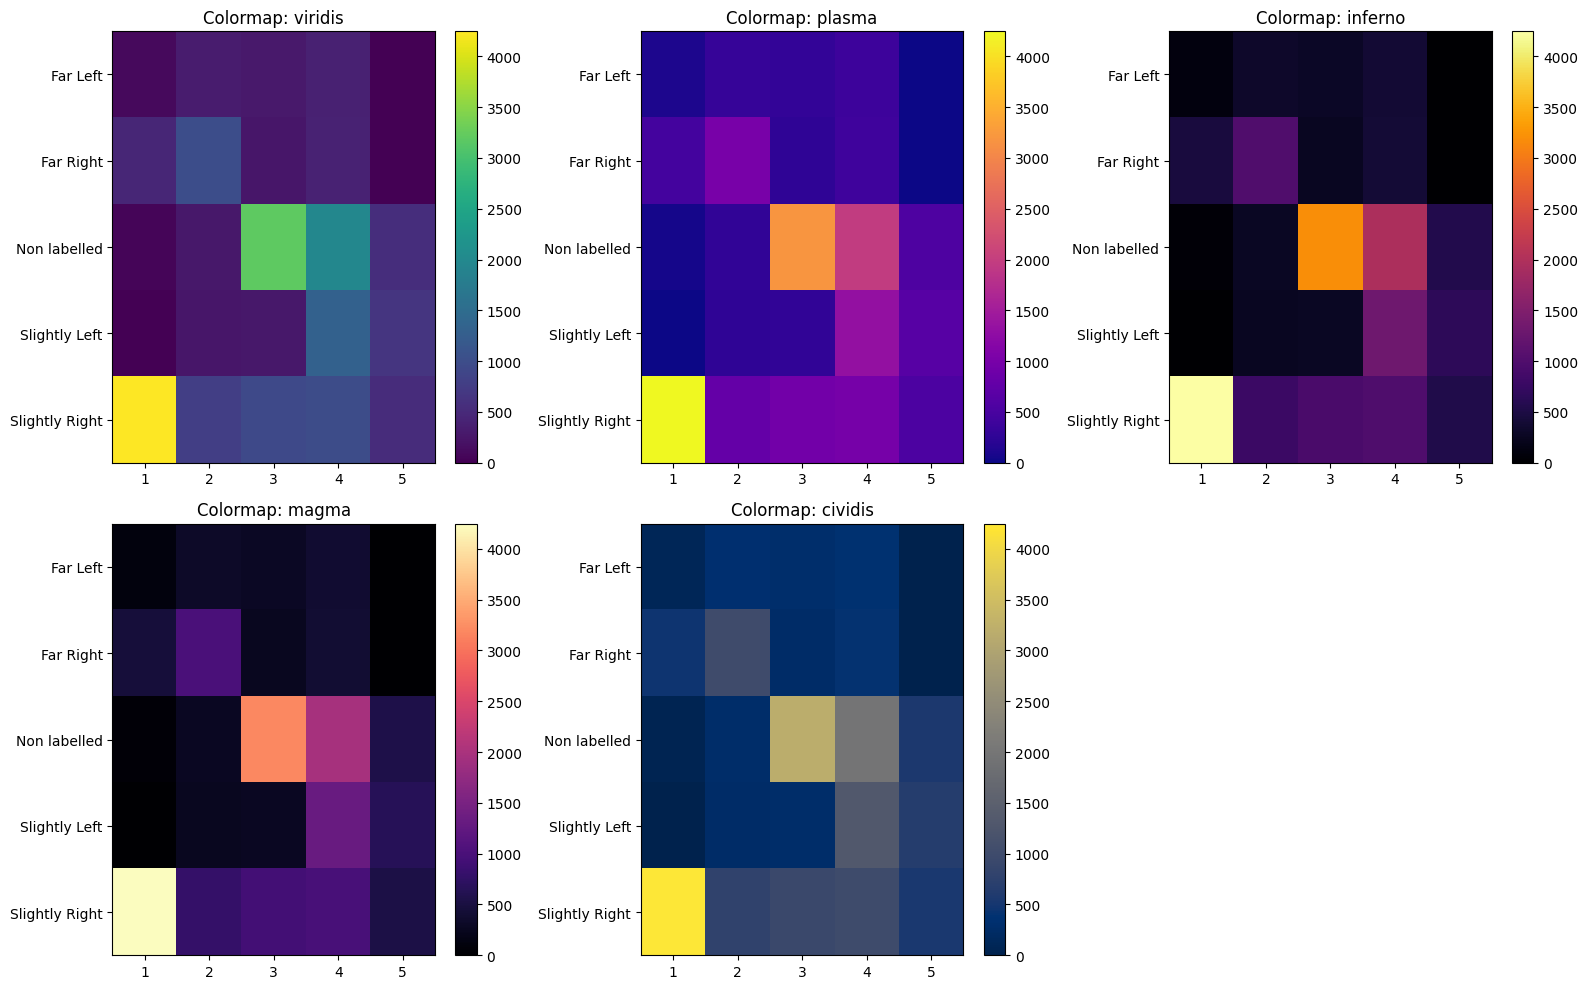
\includegraphics[width=1\columnwidth]{img/heatmap_article_distribution.png}
%     \caption{Distribution of political leanings for each predicted label. Bar colors indicate different reliability labels, while distinct hatch patterns represent the specific political leanings.
% \label{fig:cherobae'?}
%     }    
% \end{figure}

% \begin{figure}[h!]
%     \centering
%     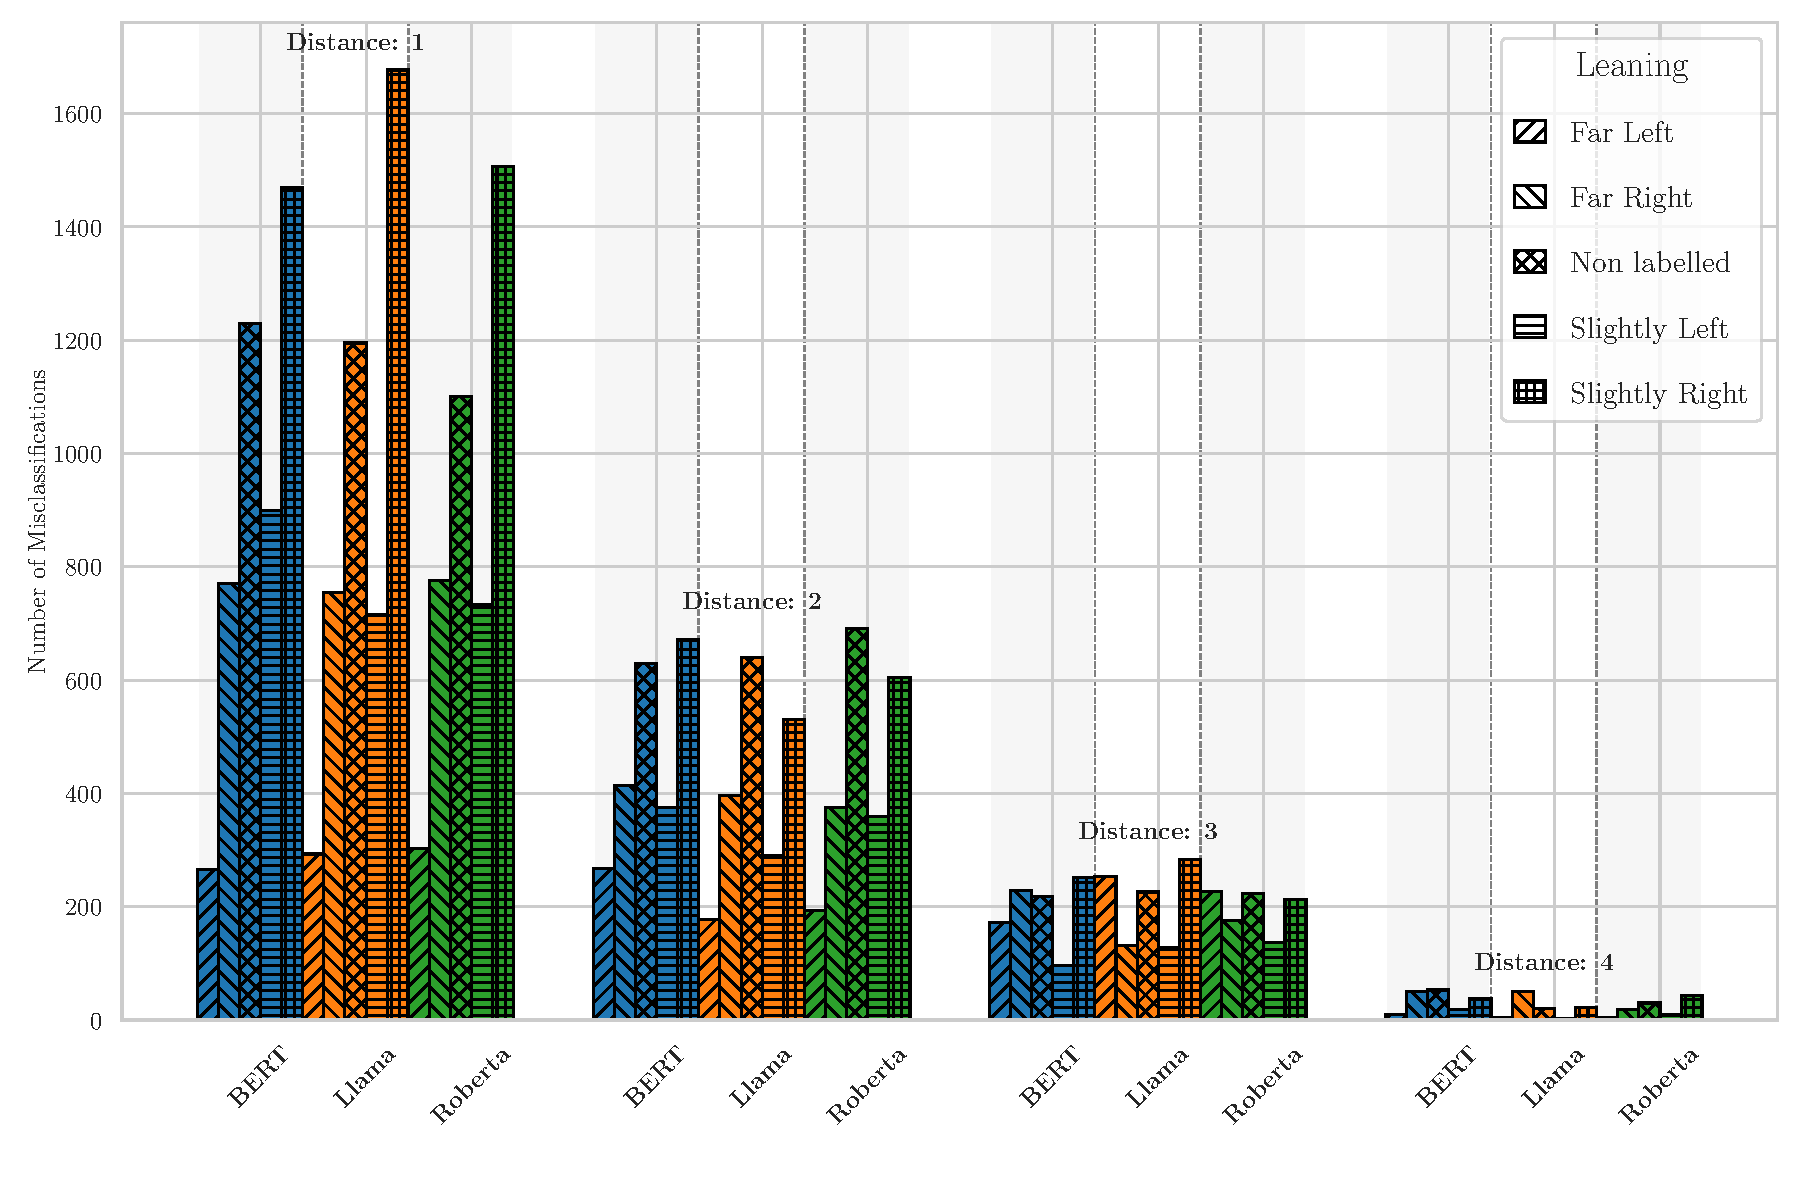
\includegraphics[width=1\columnwidth]{img/Error-Chart.pdf}
%     \caption{The bar chart shows the number of misclassification errors, for each absolute distance value from the correct score range, classified according to political orientation (e.g., left or right orientation) and organized by model.}
%     \label{fig:errorsDistribution}
% \end{figure}


% To gain further insight into the models' predictions, we consider the political leaning of the news outlets. \textcolor{blue}{In particular, we want to understand whether models are influenced by the political leaning of the news outlet in their decisions regarding its reliability.}






% \{In che modo faremo luce su questo aspetto? Scriverei già qui gli aspetti importanti che vogliamo esplorare, (gli esperimenti serviranno a far luce su quei particolari aspetti). Penso possa servire per creare un filo conduttore e rafforzare la narrativa di questa parte). In altre parole, qual è il messaggio dei singoli esperimenti condotti che combinati ci fanno rispondere alla domanda del paragrafo?}

% \{ANTICIPEREI MESSAGGIO FIG? Anticiperei cosa si vede e.g., osserviamo che gli errori NON sono uniformi across political leaning? Infatti dalla figura \dots questo sbilanciamento e' statisticamente rilevante? ed andrei con le misure statistiche \dots se si, è statisticamente rilevante la differenza vediamo come il modello sbaglia a seconda del political leaning, per singolo orientamento (o raggruppamenti 'far left/right vs. altri', 'con vs. senza political leaning', etc) il modello tende a sovrastimare o penalizzare? (Fig. 6) Dove di preciso? (- matrici Fig. 10), ci sono dei pattern a comune tra i modelli? O si osserva qualcosa di diverso in qualche modello? \{Dalla figura puoi fare un guess? Ma ci sono tutti i test dopo che te lo dicono - questo è lo stato, ci fa venire il dubbio, facciamo altre prove, ancora non siamo sicuri, facciamo i test.}}

% The information about the political leaning of the news outlet is also taken from NewsGuard. \{As for the reliability score,} we transfer the political label assigned to the news outlet to the individual news items from that outlet. Thus, with a slight abuse of notation, we discuss articles that are slightly left, slightly right, and so on, when in reality they originate from news outlets labeled accordingly.
% % Our focus is on prediction errors and the distance between the exact and predicted classes (for example, a correct label of 4 and a predicted label of 2 represents an error with a distance of 2).
% \textcolor{blue}{For the analysis, we aggregate the predictions generated across the five test folds of the \{stratified} cross-validation procedure described above. This allows us to evaluate the entire dataset and also without bias, as each prediction was produced by a model that had not been trained on the corresponding sample. 
% % All results presented in this section aggregate predictions from the five test folds of the cross-validation procedure that covers the entire dataset.
% }
% %\{For the analysis, we leverage predictions obtained for the entire article dataset. Specifically, for each model, we aggregate reliability predictions from the test folds of the stratified 5-fold cross-validation procedure, combining them one fold at a time. This yields unbiased predictions for all samples, as each prediction is generated by a model that was not trained on the corresponding instance.}
% % \{fino a qui.}

% % This section analyzes the distribution of misclassifications across the 5 test folds, examining errors based on the distance between correct and predicted values. For instance, a correct label of 4 and a predicted label of 2 represents an error with a distance of 2. We conducted this analysis to determine if newspaper orientation influences prediction accuracy, specifically investigating its contribution to model errors. Naturally, errors with greater distances should be considered more critical than those with closer distances. 

% Figure \ref{fig:orientationDistribution} shows the distribution of the political leanings of the news outlets across the five reliability labels. As we can see, Label 1 is heavily dominated by the 'Slightly Right' leaning (4,245 instances), while 'Far Left', 'Slightly Left' (0 instances), and non-labeled news are minimally represented in this category. Label 2 is primarily composed of 'Far Right' (999) and 'Slightly Right' (782) articles. Label 3 and Label 4 are characterized by a high volume of non-labeled articles (3,189 and 1,964, respectively). Additionally, Label 4 contains a significant cluster of 'Slightly Left' articles (1,325). Label 5 contains the fewest total articles; it is relatively balanced between 'Slightly Left' (663), non-labeled (563), and 'Slightly Right' (542) articles, and contains zero 'Far Right' instances. 

% % Figure \ref{fig:errorsDistribution} shows the misclassification errors and their distance for each model, grouped according to the political leaning of the news media.

% % % Conversely, Label 3 frequently includes non-labelled articles (1965 instances) and Slightly Left (1721 instances) orientations. Label 2 is also notably dominated by non-labelled orientations (3190 instances), suggesting a strong association between this label and untagged orientation values in the NewsGuard dataset. 

% % Figure \ref{fig:errorsDistribution} shows the prediction errors for each model, grouped by the political orientation of the news outlet to which the article belongs and by distance from the correct label.

% % At Distance 1, all models exhibit their highest misclassification rates, particularly for 'Slightly Right' leaning and 'Non labelled' articles. In this category, Llama recorded the highest volume of errors for 'Slightly Right' (1677), followed by RoBERTa (1506) and BERT (1469). 'Non labelled' articles also contributed significantly to the error count at this distance, with all models exceeding 1100 misclassifications. As the distance increases, the total number of misclassifications decreases significantly across all models and leanings. Distance 4 consistently represents the lowest error rates, with 'Far Left' orientations showing minimal misclassifications for all models (e.g., BERT: 10; Llama: 5; RoBERTa: 4).

 
% \textcolor{blue}{Figure \ref{fig:politicalErrorRates} presents error rates stratified by political leaning. The rate is calculated as the mean of binary misclassification scores (where 0 denotes a correct prediction and 1 denotes an error). Thus, a value of 0.4 corresponds to a 40\% failure rate for that specific group. All three models consistently struggle with `Far Left' and `Far Right' articles, achieving error rates between 62\% and 72\%. `Non labelled' and `Slightly Right' articles exhibit the lowest error rates (31-33\%), and  `Slightly Left' articles fall in the intermediate range (47-58\%). 
% % This pattern holds true for all models, despite their differing architectures. 
% % Thus, we will have a closer look at the relationship between political orientation and how the models' predict the source's reliability.
% }
% The elevated error rates for articles with the two extreme political leanings cannot be attributed to sample size effects only. In fact, although the models find it more difficult to predict the reliability level of `Far Left' and `Far Right' articles (which are, resp.  1,015 and 2,142 articles), 
% the `Slightly Left' category, which has a similar sample size to `Far Right', has lower classification error rates (47–58\% compared with 62–68\%). This suggests that the increased error rates cannot be explained solely by differences in sample size and that political leaning could influence the performance of the models.

% % extremity correlates with classification difficulty independent of model design.


% \sout{\textcolor{blue}{For a more detailed understanding of how political orientation affects model performance, we provide confusion matrices for each political leaning category in the Appendix, Figure \ref{fig:cmPoliticalLeaning}). \{devo capire dove mettere questo riferimento}}}


% \textcolor{blue}{In Figure~\ref{fig:politicalErrorsDirection}, we report the direction of misclassifications, computed as the mean signed difference between the predicted and true reliability class, by political leaning. 
% % the algebraic sum of the distances from the correct reliability class divided by the number of errors, 
% To clarify further, let the reader assume to have 5 classification errors for the reliability $l_3$ and political leaning x. Specifically, two predictions are in $l_2$, therefore at a distance of -1 from $l_3$, one prediction is in $l_1$ (distance -2), and two predictions are in $l_4$ (distance +1). 
% Therefore, the average misclassification value is equal to (-1-1-2+1+1) / 5 = -0.4. The direction is negative, meaning that the model tends to underestimate the reliability class for that set of articles.}
% % the mean signed difference between the predicted and true reliability class. 
% % For example, a value of $+1$ corresponds to an average overestimation by one reliability level and $-1$ to an underestimation by one level.

% The results highlight consistent directional patterns across the three models. `Far Left' articles are overestimated, with average positive values ranging from 0.46 (BERT) to 0.63 (Llama). A similar trend is observed for `Far Right' articles, which are consistently overestimated, with mean errors spanning from 0.52 to 1.00 across models, indicating overestimations approaching one full reliability level. `Slightly Left' articles exhibit underestimation, with average error values of 0.60 (Llama), 0.73 (RoBERTa), and 0.82 (BERT).
% For `Slightly Right' and `Non-labelled' articles, the misclassification errors are generally smaller in magnitude than for the other leanings, and the behaviour of the models is less consistent. For example, Llama and RoBERTa slightly underestimate the reliability of `Slightly Right' news outlets, whereas BERT slightly overestimates it. A similar pattern emerges for the `non-labelled' category. BERT and Llama demonstrate a slight positive bias, whereas RoBERTa's average error is close to zero.
% % 'Non labelled' and 'Slightly Right' articles exhibit near-zero bias, indicating balanced errors.

% % \textcolor{blue}{These directional biases suggest that models associate extreme political orientations with higher reliability scores than warranted. This pattern is particularly pronounced for 'Far Left' and 'Far Right' outlets, where models consistently predict reliability scores 0.5-1.0 labels higher than the true values. Conversely, 'Slightly Left' outlets are consistently perceived as less reliable than they actually are, with an underestimation of approximately 0.6-0.8 labels across all models.}



% % sample contains only  articles, and presen 'Far Right' includes  samples, comparable to 'Slightly Left' (2,407 samples), yet exhibits significantly worse performance (62-68\% error rate versus 47-58\%). This indicates that classification difficulty stems from inherent characteristics of extreme political orientations rather than data scarcity.}

% % To assess whether the observed differences in error rates across political orientations are statistically significant, we perform chi-square tests of independence for each model. Table \ref{tab:chi_square_results} reports the results.

% \{
%  To assess whether classification errors are systematically associated with political leaning, we conduct a chi-square ($\chi^2$) test of independence between political leaning and classification outcome (correct vs.\ incorrect) for each model.
% Formally, for each model, we test the null hypothesis
% \begin{equation}
% H_0: \text{Errors in reliability classification are independent of political leaning.
% },
% \end{equation}
% against the alternative hypothesis
% \begin{equation}
% H_1: \text{Errors in reliability classification depend on political leaning.
% }.
% \end{equation}
% The $\chi^2$ test compares the observed contingency table, which reports, for each political leaning, how many articles were classified correctly or incorrectly, with the expected contingency table obtained under the assumption of independence. In this table, each cell $O_{ij}$ contains the number of articles belonging to political leaning $i$ with classification outcome $j$ (correct or incorrect). The corresponding expected value $E_{ij}$ represents how many articles would fall into that cell $(i,j)$ if political leaning had no relationship to classification accuracy. The test statistic is then computed as
% \begin{equation}
% \chi^2 = \sum_{i} \sum_{j} \frac{(O_{ij} - E_{ij})^2}{E_{ij}}.
% \end{equation}

% % The $\chi^2$ test compares the observed contingency table  of error counts with the expected counts under the assumption of independence. The test statistic is defined as
% % \begin{equation}
% % \chi^2 = \sum_{i,j} \frac{(O_{ij} - E_{ij})^2}{E_{ij}},
% % \end{equation}
% % where $O_{ij}$ and $E_{ij}$ denote the observed and expected frequencies for political orientation $i$ and classification outcome $j$, respectively. In particular, $E_{ij}$ represents the number of errors (or correct predictions) expected under the null hypothesis that political orientation and classification outcome are independent.
% % In addition to the $\chi^2$ statistic and its associated $p$-value, we report {Cramér’s V index, a normalized effect-size measure that quantifies the strength of the dependence between political orientation and reliability classification errors, independently of the sample size:
% % \begin{equation}
% % V = \sqrt{\frac{\chi^2}{N \cdot \min(r-1, c-1)}},
% % \end{equation}
% % where $N$ is the total number of samples and $r$ and $c$ denote the number of rows and columns in the contingency table. 
% % Thus, the $p$-value assesses the statistical significance, and Cramér’s V measures the magnitude of the dependence between political orientation and the distribution of reliability classification errors. 
% In addition to the $\chi^2$ test and its associated $p$-value, we report Cramér’s V, a normalized effect-size measure that quantifies the strength of the dependence between political leaning and reliability classification errors, independently of the sample size:
% \begin{equation}
% V = \sqrt{\frac{\chi^2}{N \cdot \min(r-1, c-1)}},
% \end{equation}
% where $N$ is the total number of samples and $r$ and $c$ denote the number of rows (5 in our case, the political leaning) and columns (2 in our case, correct/incorrect) in the contingency table. While the $p$-value evaluates whether the association detected by the $\chi^2$ test is statistically significant, Cramér’s V indicates \emph{how strong} that association is. In fact, the $\chi^2$ statistic is highly sensitive to sample size: with very large datasets, even extremely small effects may lead to highly $\chi^2$ values. 
% Cramér’s V therefore complements the hypothesis test by providing an interpretable measure of how strongly reliability prediction errors are associated with the political leanings: values close to zero indicate that errors are distributed similarly across all political leanings, whereas values approaching one denote a near-perfect dependence, meaning that the likelihood of reliability misclassification varies almost entirely as a function of political leaning.
% Both results are reported in Table \ref{tab:chi_square_results}.

% % Cramér’s V therefore complements the hypothesis test by providing an interpretable effect size, where values close to zero indicate no association and values approaching one indicate a perfect association.


% \begin{table}[t]
% \centering
% \begin{tabular}{lcccc}
% \textbf{Model} & \textbf{Accuracy} & $\boldsymbol{\chi^2}$ & \textbf{$p$-value} & \textbf{Cramér’s V} \\
% \midrule
% BERT    & 58.27\% & 1684.13 & $<10^{-300}$ & 0.294 \\
% RoBERTa & 60.34\% & 1418.31 & $<10^{-300}$ & 0.270 \\
% Llama   & 59.97\% & 1207.83 & $<10^{-250}$ & 0.249 \\
% \end{tabular}
% \caption{\{Questi sono test di cosa?} {\sout{Results of chi-square test, with p-values associated, and Cramer's V tests. Extremely small $p$-values arise due to the large sample size. Cramér’s V quantifies the strength of the dependence between political leaning and misclassification behavior.}} Statistical tests for Political Leaning vs. Classification Correctness. The table reports the Chi-square ($\chi^2$) test of independence and the associated $p$-values to assess whether error rates vary across political orientations. Cramér’s V is provided to measure the effect size of this association}
% \label{tab:chi_square_results}
% \end{table}



% Across all models, the $\chi^2$ tests yield extremely small $p$-values, leading to a clear rejection of the null hypothesis of independence. This indicates that classification errors are \emph{not uniformly distributed} across political orientations.

% As said, the absolute magnitude of the $\chi^2$ statistic is primarily driven by sample size and therefore is not directly interpretable as a measure of effect strength; for this reason, we rely on Cramér’s V to quantify the magnitude of the association.
% The values of Cramér’s V range from 0.249 to 0.294, corresponding to \emph{small-to-moderate and consistent associations} between political leaning and misclassification behavior across models. Among the evaluated architectures, BERT exhibits the strongest association ($V = 0.294$), followed by RoBERTa ($V = 0.270$) and Llama ($V = 0.249$). While the differences in Cramér’s V are moderate, they suggest that political leaning contributes more to explaining the variability of BERT’s errors than those of RoBERTa or Llama, with comparatively more uneven error distributions across political leanings.

% To identify which political orientations contribute most to the observed dependence, we analyze the \emph{cell-wise} contributions to the $\chi^2$ statistic, where each cell corresponds to a specific combination of political orientation $i$ and classification outcome $j$, computing how far the observed number of errors deviates from what would be expected under independence, as follows: 
% \begin{equation}
% \frac{(O_{ij} - E_{ij})^2}{E_{ij}}.
% \end{equation}

% This analysis reveals that the majority of the $\chi^2$ mass is consistently driven by `Far Left' and `Far Right'. For instance, in the BERT model, errors associated with `Far Right' and `Far Left' orientations contribute 363.73 and 201.94, respectively, to the overall $\chi^2$ statistic, substantially exceeding the contributions of moderate or non-labelled orientations. The same pattern is observed for Llama (`Far Right': 263.64, `Far Left': 257.79) and RoBERTa (`Far Right': 287.86, `Far Left': 261.53).

% These consistently large contributions correspond to large standardized residuals, indicating that errors on extreme political orientation content occur significantly more frequently than expected under the assumption of independence.

% \{da rivedere}
% Overall, these results demonstrate that political orientation systematically affects model performance across all evaluated architectures. The consistency of effect sizes and contribution patterns across models suggests that the observed dependence is unlikely to stem from specific architectural choices. Instead, it plausibly reflects intrinsic differences in linguistic style, framing, or topical structure across ideological extremes, which pose greater challenges for current models.}

% \textcolor{blue}{Therefore, we study whether the observed differences in error rates across political orientations are statistically significant through chi-square tests \cite{citazione} of independence for each model. We report the results of these tests in \ref{tab:chi_square_results}. 
% }

% \begin{table}[h!]
% \centering
% \begin{tabular}{lcccc}
% \textbf{Model} & \textbf{Accuracy} & \textbf{$\chi^2$} & \textbf{P-Value} & \textbf{Cramér's V} \\
% \hline
% BERT    & 58.27\% & 1684.13 & $< 10^{-300}$ & 0.294 \\
% Llama   & 59.97\% & 1207.83 & $< 10^{-250}$ & 0.249 \\
% RoBERTa & 60.34\% & 1418.31 & $< 10^{-300}$ & 0.270 \\
% \end{tabular}
% \caption{\textcolor{blue}{Chi-square test results assessing the dependence between political orientation and classification errors. Extremely large sample sizes produce small p-values, while Cramér's V quantifies the practical effect size.}}
% \label{tab:chi_square_results}
% \end{table}

% \textcolor{blue}{Across all models, the chi-square tests produce extremely small p-values (effectively zero at machine precision), indicating that classification errors are not evenly distributed across political orientations. However, because the dataset is large, statistical significance alone is insufficient to inform about the magnitude of the dependence. Cramér's V provides this information: the effect sizes range from 0.249 to 0.294, corresponding to small and consistent associations between political orientation and misclassification patterns. BERT shows the strongest dependence (V = 0.294), followed by RoBERTa (V = 0.270) and Llama (V = 0.249).}

% \textcolor{blue}{Inspection of the per-cell contributions to the chi-square statistic reveals that the vast majority of the dependence is driven again by the 'Far Right' and 'Far Left' categories. For example, in BERT, 'Far Right' errors contribute 363.73 and 'Far Left' errors contribute 201.94 to the chi-square statistic, far exceeding contributions from moderate or unlabelled orientations. Llama and RoBERTa exhibit the same pattern (Llama: Far Right = 263.64, Far Left = 257.79; RoBERTa: Far Right = 287.86, Far Left = 261.53). These consistently large residuals indicate that models make disproportionately more errors on ideologically extreme content than expected under the assumption of independence.}

% \textcolor{blue}{Taken together, these findings show that political orientation systematically affects model performance across BERT, Llama, and RoBERTa. The consistent pattern suggests that the bias arises from properties intrinsic to the data or linguistic differences across ideological content rather than from specific architectural features.}


% \section{Political Leaning  e }

% To further investigate the models’ reliability predictions, we analyze the role of the political leaning of news outlets. Specifically, we assess whether political orientation systematically influences model performance, both in terms of error frequency and error direction.

% Political leaning labels are obtained from NewsGuard and assigned at the outlet level. These labels are transferred to individual articles published by each outlet. With a slight abuse of notation, we therefore refer to articles as \emph{Far Left}, \emph{Slightly Left}, and so on, according to their source’s political orientation.

% Figure~\ref{fig:orientationDistributionInverted} reports the distribution of reliability labels across political leanings. The distribution is markedly imbalanced: reliability classes are not uniformly represented within each political category, and some leanings (e.g., \emph{Far Right} and \emph{Slightly Left}) exhibit incomplete coverage across reliability levels. This imbalance constitutes a structural property of the dataset that must be accounted for when interpreting model errors.

% \subsection{Error Frequency by Political Leaning}

% Figure~\ref{fig:politicalErrorRates} shows the error rates stratified by political leaning and model. Error rates are computed as the mean of a binary misclassification indicator (0 = correct, 1 = incorrect), such that a value of 0.4 corresponds to a 40\% error rate.

% Across all models, error rates vary substantially with political leaning and follow consistent patterns. Articles from politically extreme outlets (\emph{Far Left} and \emph{Far Right}) are the most challenging, with error rates ranging between 62\% and 72\%. In contrast, \emph{Non-labelled} and \emph{Slightly Right} articles exhibit the lowest error rates (31--33\%), while \emph{Slightly Left} articles fall in an intermediate range (47--58\%), closer to the extremes than to moderate categories.

% To formally assess whether misclassification frequency depends on political leaning, we conduct a chi-square ($\chi^2$) test of independence between political orientation and classification outcome (correct vs.\ incorrect) for each model. Table~\ref{tab:chi_square_results} reports the results. In all cases, the association is statistically significant, with moderate effect sizes as measured by Cramér’s V, indicating a non-negligible dependence between political leaning and error occurrence.
% For a more granular analysis of these results, we provide the full confusion matrices for BERT, Llama, and RoBERTa stratified by political leaning in the Appendix (see Figures~\ref{fig:cmPoliticalLeaningBert}, \ref{fig:cmPoliticalLeaningLlama}, and \ref{fig:cmPoliticalLeaningRoberta}).

% \subsection{Direction of Errors}

% Beyond error frequency, we examine whether models exhibit systematic biases in the \emph{direction} of their misclassifications. Figure~\ref{fig:politicalErrorsDirection} reports the mean signed difference between predicted and true reliability labels, stratified by political leaning. Positive values indicate overestimation of reliability, while negative values indicate underestimation.

% All three models display highly consistent directional patterns. Articles from politically extreme outlets are systematically overestimated: \emph{Far Left} articles show mean positive errors ranging from 0.46 (BERT) to 0.63 (Llama), while \emph{Far Right} articles exhibit even stronger overestimation, with mean errors between 0.52 and 1.00, approaching one full reliability level.

% In contrast, \emph{Slightly Left} articles are consistently underestimated across models, with average errors of 0.60 (Llama), 0.73 (RoBERTa), and 0.82 (BERT). For moderate categories (\emph{Slightly Right} and \emph{Non-labelled}), error magnitudes are smaller and less consistent across models. BERT tends to slightly overestimate reliability, whereas Llama and RoBERTa show mild underestimation or near-zero bias.

% Overall, the results show that political leaning affects not just error rates, but the direction of the errors themselves. These systematic tendencies to over- or under-estimate are strongest at the ends of the political spectrum.







% \subsection{Influence of Political Leaning on Classification Errors}
% % -------------------------------------------------------------------------
% % Commenti 
% % 1. "credo che questa parte sia poco chiara.. quale messaggio vogliamo lasciare al lettore?"
% % 2. "publisher or article? direi che qui va specificato che il valore di leaning è sul publisher originariamente e poi viene affrontato qui analizzando il leaning del publisher degli articoli classificati"
% % 3. "cosa si intende per 'contextualize the dataset and potential confounding factors'?"
% % -------------------------------------------------------------------------

% The reliability labels provided by NewsGuard often correlate with editorial practices that reflect a news outlet's political stance. 
% The core objective of this section is to determine if our models exhibit political bias. Specifically, we investigate whether the models treat all sides of the political spectrum equally or if they systematically penalize specific orientations.

% It is important to clarify the level of analysis. Political orientation is a property of the publisher (domain), not the individual text. However, since our models operate at the article level, we assign the publisher's political label to every article it produces. This allows us to analyze how the source's political alignment influences the prediction errors on its content.

% Our analysis proceeds in three steps:

% \begin{enumerate}
%     \item \textbf{Distribution Analysis.} First, we map how political orientations are distributed across reliability classes (Figure \ref{fig:orientationDistributionInverted}). This step is crucial to identify structural imbalances. For example, if all "Far Left" outlets in our dataset also happen to be "Low Reliability," the model might learn a correlation between politics and trust. We need to expose these overlaps to interpret results correctly.
    
%     \item \textbf{Error Rate Analysis.} Second, we assess if the models find it harder to classify articles from specific political groups (Figure \ref{fig:politicalErrorRates} and Table \ref{tab:chi_square_results}). We test if error rates are significantly higher for any orientation.
    
%     \item \textbf{Directional Bias Analysis.} Finally, we examine the \textit{direction} of the mistakes (Figure \ref{fig:politicalErrorsDirection}). We ask: when the model is wrong, does it tend to overestimate reliability (positive bias) or underestimate it (negative bias) depending on the political leaning?
% \end{enumerate}

% Together, these experiments reveal whether the models behave uniformly across the spectrum or if notable political patterns emerge.


% \subsubsection{Error rates across political orientations}\label{subsec:politicalErrorRates}
% Given the significant imbalance across political orientations in the dataset, we analyze model errors by calculating rates independently for each leaning category. These error rates are computed per orientation as the ratio of incorrect predictions to the total number of predictions within that class (i.e., the mean of a binary variable where 1 denotes an error and 0 a correct prediction), making them independent of class frequency and allowing us to study model errors despite the overall dataset imbalance.
% Figure \ref{fig:politicalErrorRates} shows the mean misclassification rate for each model and orientation. All models exhibit substantially higher error rates for articles from Far Left and Far Right outlets, with values ranging from 62\% to 72\%, compared to substantially lower rates for Slightly Right and non-labelled outlets (31--33\%) and intermediate rates for Slightly Left articles (47--58\%).

% \sout{It is important to note that these differences cannot be explained solely by sample size effects. For instance, although the Slightly Left category is comparable in size to Far Right, its error rates are notably lower. In order to formally assess whether error rates depend on political orientation, we apply a chi-square test of independence between political leaning and classification correctness. For all models, the null hypothesis of independence \{(i.e., \dots)} is decisively rejected (see Table \ref{tab:chi_square_results}), indicating that misclassification frequency is not uniformly distributed across political orientations. Cramer's V further confirms a small-to-moderate but consistent association between leaning and error behavior.}

% Crucially, these disparities are not merely artifacts of data scarcity. For instance, although the \textit{Slightly Left} and \textit{Far Right} categories differ in sample size, the difference in their error rates is disproportionate to their volume, suggesting a structural difficulty rather than a lack of training data.  To formally validate this, we apply a Chi-square test of independence. The null hypothesis states that classification correctness is independent of political leaning (i.e., the probability of making an error should be the same regardless of the publisher's orientation). For all models, this hypothesis is decisively rejected (see Table \ref{tab:chi_square_results}), confirming that misclassification frequency is significantly tied to political stance. Cramer's V further confirms a small-to-moderate consistent association.



% \subsubsection{Direction of misclassifications}

% Error frequency alone does not reveal whether models systematically shift predictions toward a specific end of the political spectrum. To investigate this, we compute the mean signed error (predicted label minus true label), specifically for misclassified instances (calculated as the sum of signed errors divided by the total number of misclassifications for each orientation). 
% \sout{In our numerical encoding, positive values indicate a bias toward the right (overestimation), whi    le negative values indicate a bias toward the left (underestimation).}
% In our numerical encoding (where $l_5$ represents maximum credibility), positive values indicate overestimation (bias toward higher reliability scores), while negative values indicate underestimation (bias toward lower reliability scores).

% Clear directional patterns emerge across all three models.  Far Left and Far Right articles exhibit consistent overestimation, with mean signed errors ranging from +0.46 to +1.00, approaching a full reliability level.

% Slightly Left articles show systematic underestimation, with average values between –0.60 and –0.82.

% Slightly Right and non-labelled outlets display smaller, less consistent deviations: Llama and RoBEETa slightly underestimate 
% Slightly Right reliability, whereas BERT slightly overestimates it; for non-labelled outlets, BERT and Llama exhibit mild positive biases while RoBERTa's average bias is near zero.

% These results indicate that models not only differ in error frequency across political orientations but also in error direction, suggesting that some political groups are systematically pushed toward higher or lower predicted reliability levels.

% \subsubsection{Identifying the orientations driving dependence}

% \sout{To better understand which political orientations contribute most to the statistical dependence identified by the chi-square test, we examine the cell-wise contributions to the chi-square statistic \mbox{(\ref{app:political_cms})}. This analysis confirms that the largest deviations from expected values occur for Far Left and Far Right orientations, which contribute disproportionately to the overall test statistic. Slightly Left also shows substantial contributions, consistent with the systematic underestimation pattern identified above. These findings underscore that extreme political orientations are the primary drivers of the observed dependence between political leaning and classification correctness.}

% To better understand which political orientations are responsible for this statistical dependence, we examine the detailed confusion matrices broken down by leaning (visualized in \ref{app:political_cms}).
% By analyzing the specific error distributions in these matrices, we can pinpoint where the "observed" errors drastically exceed the "expected" statistical baseline. The visualization confirms that Far Left and Far Right orientations are the primary drivers of the anomaly: their corresponding sections in the matrices exhibit high off-diagonal values (misclassifications) that contribute disproportionately to the total Chi-square score. 
% \textit{Slightly Left} also shows a notable deviation, consistent with the systematic underestimation pattern identified earlier. 
% These findings clarify that the link between political leaning and classification correctness is not uniform; rather, it is heavily skewed by the model's struggle to process content from extreme political spectrums.


% \section{Conclusions}
% % 9 January, 12:20 pm
% % noi non facciamo esattamente questo, prediciamo la reliability degli articoli, non del publisher
% In this work, we addressed the problem of news source reliability prediction by investigating whether the reliability level of a publisher can be inferred from the textual content of its articles. The task was formulated as a five-class ordinal classification problem, aligned with the reliability scale adopted by professional journalistic organizations. Unlike many existing approaches that rely on metadata, social interactions, or manual inspections, our study focuses on a purely content-based and scalable formulation.

% % 9 January, 2:39 pm
% % sposterei tutto in una parte contributions
% A first major contribution of this work is the construction of a substantially expanded dataset, derived from NewsGuard and enriched with articles from previous studies. The resulting corpus comprises 19,476 political news articles from 669 English-language publishers, distributed across five reliability levels. 

% %This represents, to the best of our knowledge, one of the largest datasets specifically designed for publisher-level reliability prediction, and enables a more robust and realistic experimental evaluation.

% Second, we performed a comparison of multiple transformer-based models, including BERT, RoBERTa-large, and LLaMA3, under a five-fold cross-validation protocol. The results show that all models are capable of capturing meaningful signals associated with publisher reliability, with RoBERTa-large and LLaMA3 consistently outperforming BERT across most evaluation metrics. %This confirms the effectiveness of larger and more recent language models for this task.

% A key methodological aspect of this study is the strict separation between publishers in the training and test sets. By ensuring that test articles originate exclusively from news outlets never seen during training, we evaluate the models under a realistic deployment scenario, where the goal is to assess the reliability of previously unclassified or emerging news sources. %The strong performance achieved under this constraint demonstrates that the models learn generalizable publisher-level patterns, rather than relying on outlet-specific lexical memorization.

% To properly account for the ordinal nature of reliability labels, we adopted, alongside standard classification metrics, a tolerant accuracy measure that assigns partial credit to predictions that differ by only one adjacent reliability level. This allowed us to explicitly characterize the trade-off between traditional exact-match accuracy and tolerance-aware performance. While exact five-class prediction remains a challenging task, tolerant accuracy reveals that the models are highly effective in producing near-correct reliability assessments, which is particularly relevant for real-world applications where small deviations between adjacent reliability levels are less critical than severe misclassifications.

% Finally, we conducted an exploratory analysis of model errors with respect to the political leaning of news outlets. The results show that misclassifications are not uniformly distributed across ideological groups: politically extreme outlets tend to exhibit both higher error rates and systematic overestimation of their reliability, whereas Slightly Left outlets are more often underestimated. Slightly Right orientation and non labelled outlets display smaller and less consistent deviations. Although the magnitude of these effects is moderate, the presence of consistent patterns across models indicates that political orientation can influence how reliability signals are interpreted from textual content.

% % systematic differences in the distribution of misclassifications across ideological categories. While these findings already provide useful descriptive insights, a more comprehensive bias analysis is currently ongoing and will be the subject of future investigation.

% Overall, our results demonstrate that modern language models can support scalable and purely content-based assessment of news source reliability, even under strict generalization constraints. Rather than replacing the careful evaluation procedures carried out by journalistic organizations, the proposed approach is best positioned as a decision-support tool, capable of assisting experts in the early screening of unknown outlets and supporting large-scale media monitoring activities. 
% % 9 January, 2:39 pm
% % aggiungere in contributions
% To facilitate reproducibility and encourage further research, all fine-tuned models are publicly available (footnote \ref{fn:model_availability}).

% Future work may focus on:
% (i) extending the analysis to additional languages and media ecosystems,
% (ii) exploring training strategies that explicitly account for the ordinal distance between reliability levels, extending the current tolerant evaluation framework to the learning phase.


% \{\paragraph{Limitations} The models process the first 256 tokens of each article, potentially omitting editorial signals appearing later in the text. Reliability labels are inherited from publishers, introducing structural noise at the article level and resulting in a weakly supervised setting. Moreover, the analysis is limited to English-language political news outlets, which restricts generalizability to other languages and domains. Finally, domain-level reliability is estimated via majority voting over article predictions, a simple aggregation strategy that does not account for prediction confidence or uncertainty.}

% \section{Main Contributions}
% \label{sec:contributions}

% In response to the challenges posed by digital disinformation, this study makes the following key contributions to the field of automated assessment of news publishers' reliability.

% \begin{itemize}
%     \item \textbf{Huge Dataset and Comparison between Models} We constructed a large dataset comprising 19,476 political news articles from 669 publishers. Unlike previous studies that were restricted to smaller corpora, this scale enables a more robust evaluation. We compared standard encoders (BERT and RoBERTa) with state-of-the-art decoders (Llama), demonstrating the effectiveness of modern architectures for this task.
    
%     \item \textbf{Generalization via Strict Separation.} We imposed a strict constraint: publishers in the test set must never appear in the training set. This experimental design validates the models' ability to generalise to sources that have not been seen before, rather than merely memorising signals specific to particular outlets.
    
%     \item \textbf{Source Profiling Methodology.} We moved beyond simple article classification and demonstrated that aggregating predictions from a set of articles via majority voting produces accurate publisher-level ratings.
    
%     \item \textbf{Bias and Political Analysis.} We conducted a novel analysis of the interaction between reliability prediction and political leaning. Using statistical tests and directional error metrics, we quantified the effect of ideological orientation on model bias.
    
%     \item \textbf{Open Science.} To foster reproducibility, all fine-tuned models and code are publicly available.
% \end{itemize}

\section{Discussion and Conclusion}
\label{sec:conclusions}
In this study, we investigated whether the reliability of news publishers could be inferred from their articles. We framed the task as a five-level ordinal classification problem aligned with NewsGuard ratings and evaluated four transformer-based models, BERT, RoBERTa, Llama, and Mistral, under a strict publisher-disjoint protocol to simulate real-world deployment on unseen sources.

Our findings demonstrate that language models can capture meaningful and generalizable signals of publisher reliability. Interestingly, the substantially larger Mistral 24B does not outperform smaller architectures, suggesting that performance is limited by dataset characteristics rather than model size. Despite operating with a 1,024-token context window (four times larger than the 256-token limit used for the other models), Mistral shows no measurable gain in accuracy or F1 score. This may indicate that the cues discriminating reliable publishers are concentrated in the beginning of articles. The lack of benefit from the extended context further supports the hypothesis that increasing model size or input length alone cannot overcome limitations imposed by weak supervision. In weak supervision, each article inherits the reliability label of its publisher. Therefore, an individual article's deviation from the outlet's overall NewsGuard rating introduces label noise. Additionally, the diversity of publisher-level signals is limited. The moderate article-level accuracy should be interpreted in light of the ultimate objective of the framework. Since publisher reliability is a source-level property, individual articles provide only noisy evidence. The substantial performance gain obtained after aggregation suggests that reliability emerges more clearly when multiple articles are considered jointly. A key finding of this study is that publisher reliability should not be modeled as a property of isolated articles. Rather, it emerges as a collective signal that becomes substantially more stable and informative when evidence is aggregated across multiple articles from the same source. This observation supports a shift from article-centric formulations toward source-level inference frameworks, where article classification serves as an intermediate step rather than the final objective.


% While exact article-level prediction remains challenging, most errors are adjacent, suggesting that models rarely confuse highly unreliable outlets with highly reliable ones. Aggregating predictions at the publisher level substantially improves performance, confirming that reliability emerges more clearly as a collective signal than at the level of individual articles.

At the same time, our bias analysis reveals systematic interactions between reliability prediction and political leaning. Models tend to overestimate the reliability of politically extreme outlets and underestimate slightly left-leaning ones. While effect sizes remain moderate, these patterns highlight the need for bias-aware evaluation protocols in automated reliability assessment systems.

The study also presents important scope constraints. First, the dataset is restricted to English-language political news outlets, limiting generalizability to other linguistic and thematic ecosystems. Second, the weak supervision setting, where article labels inherit publisher-level ratings, introduces structural noise, as individual articles may deviate from their outlet's overall reliability profile. Finally, publisher-level inference relies on simple majority voting, which does not yet incorporate prediction confidence or uncertainty. %Finally, technical constraints required limiting input length to 256 tokens, potentially excluding relevant stylistic signals appearing later in longer articles.

Future research should extend this framework to multilingual settings, explore confidence-aware aggregation strategies, and develop training objectives explicitly tailored to ordinal classification. More broadly, combining content-based approaches with ecosystem-level signals, such as ownership transparency, citation networks, or audience interactions, may provide a more comprehensive and robust framework for scalable news source reliability assessment.





\bibliographystyle{IEEEtran}
\bibliography{bibliography}

% \appendix
% %\section{Confusion Matrices}
% \subsection{Model performance}
% \label{app:performance_cms}
% \textcolor{blue}{This appendix supports the article‑level reliability estimation experiment described in Section~\ref{sec:results}.The confusion matrices in Figure~\ref{fig:performance_cms} show the detailed results for each of the five cross‑validation folds and their overall average.}
% \sout{Figure \ref{fig:performance_cms} shows the confusion matrices for each fold and for the average.}

% \begin{figure*}[!t]
% \centering
% % riga 1
% \begin{subfigure}[b]{0.48\linewidth}
%   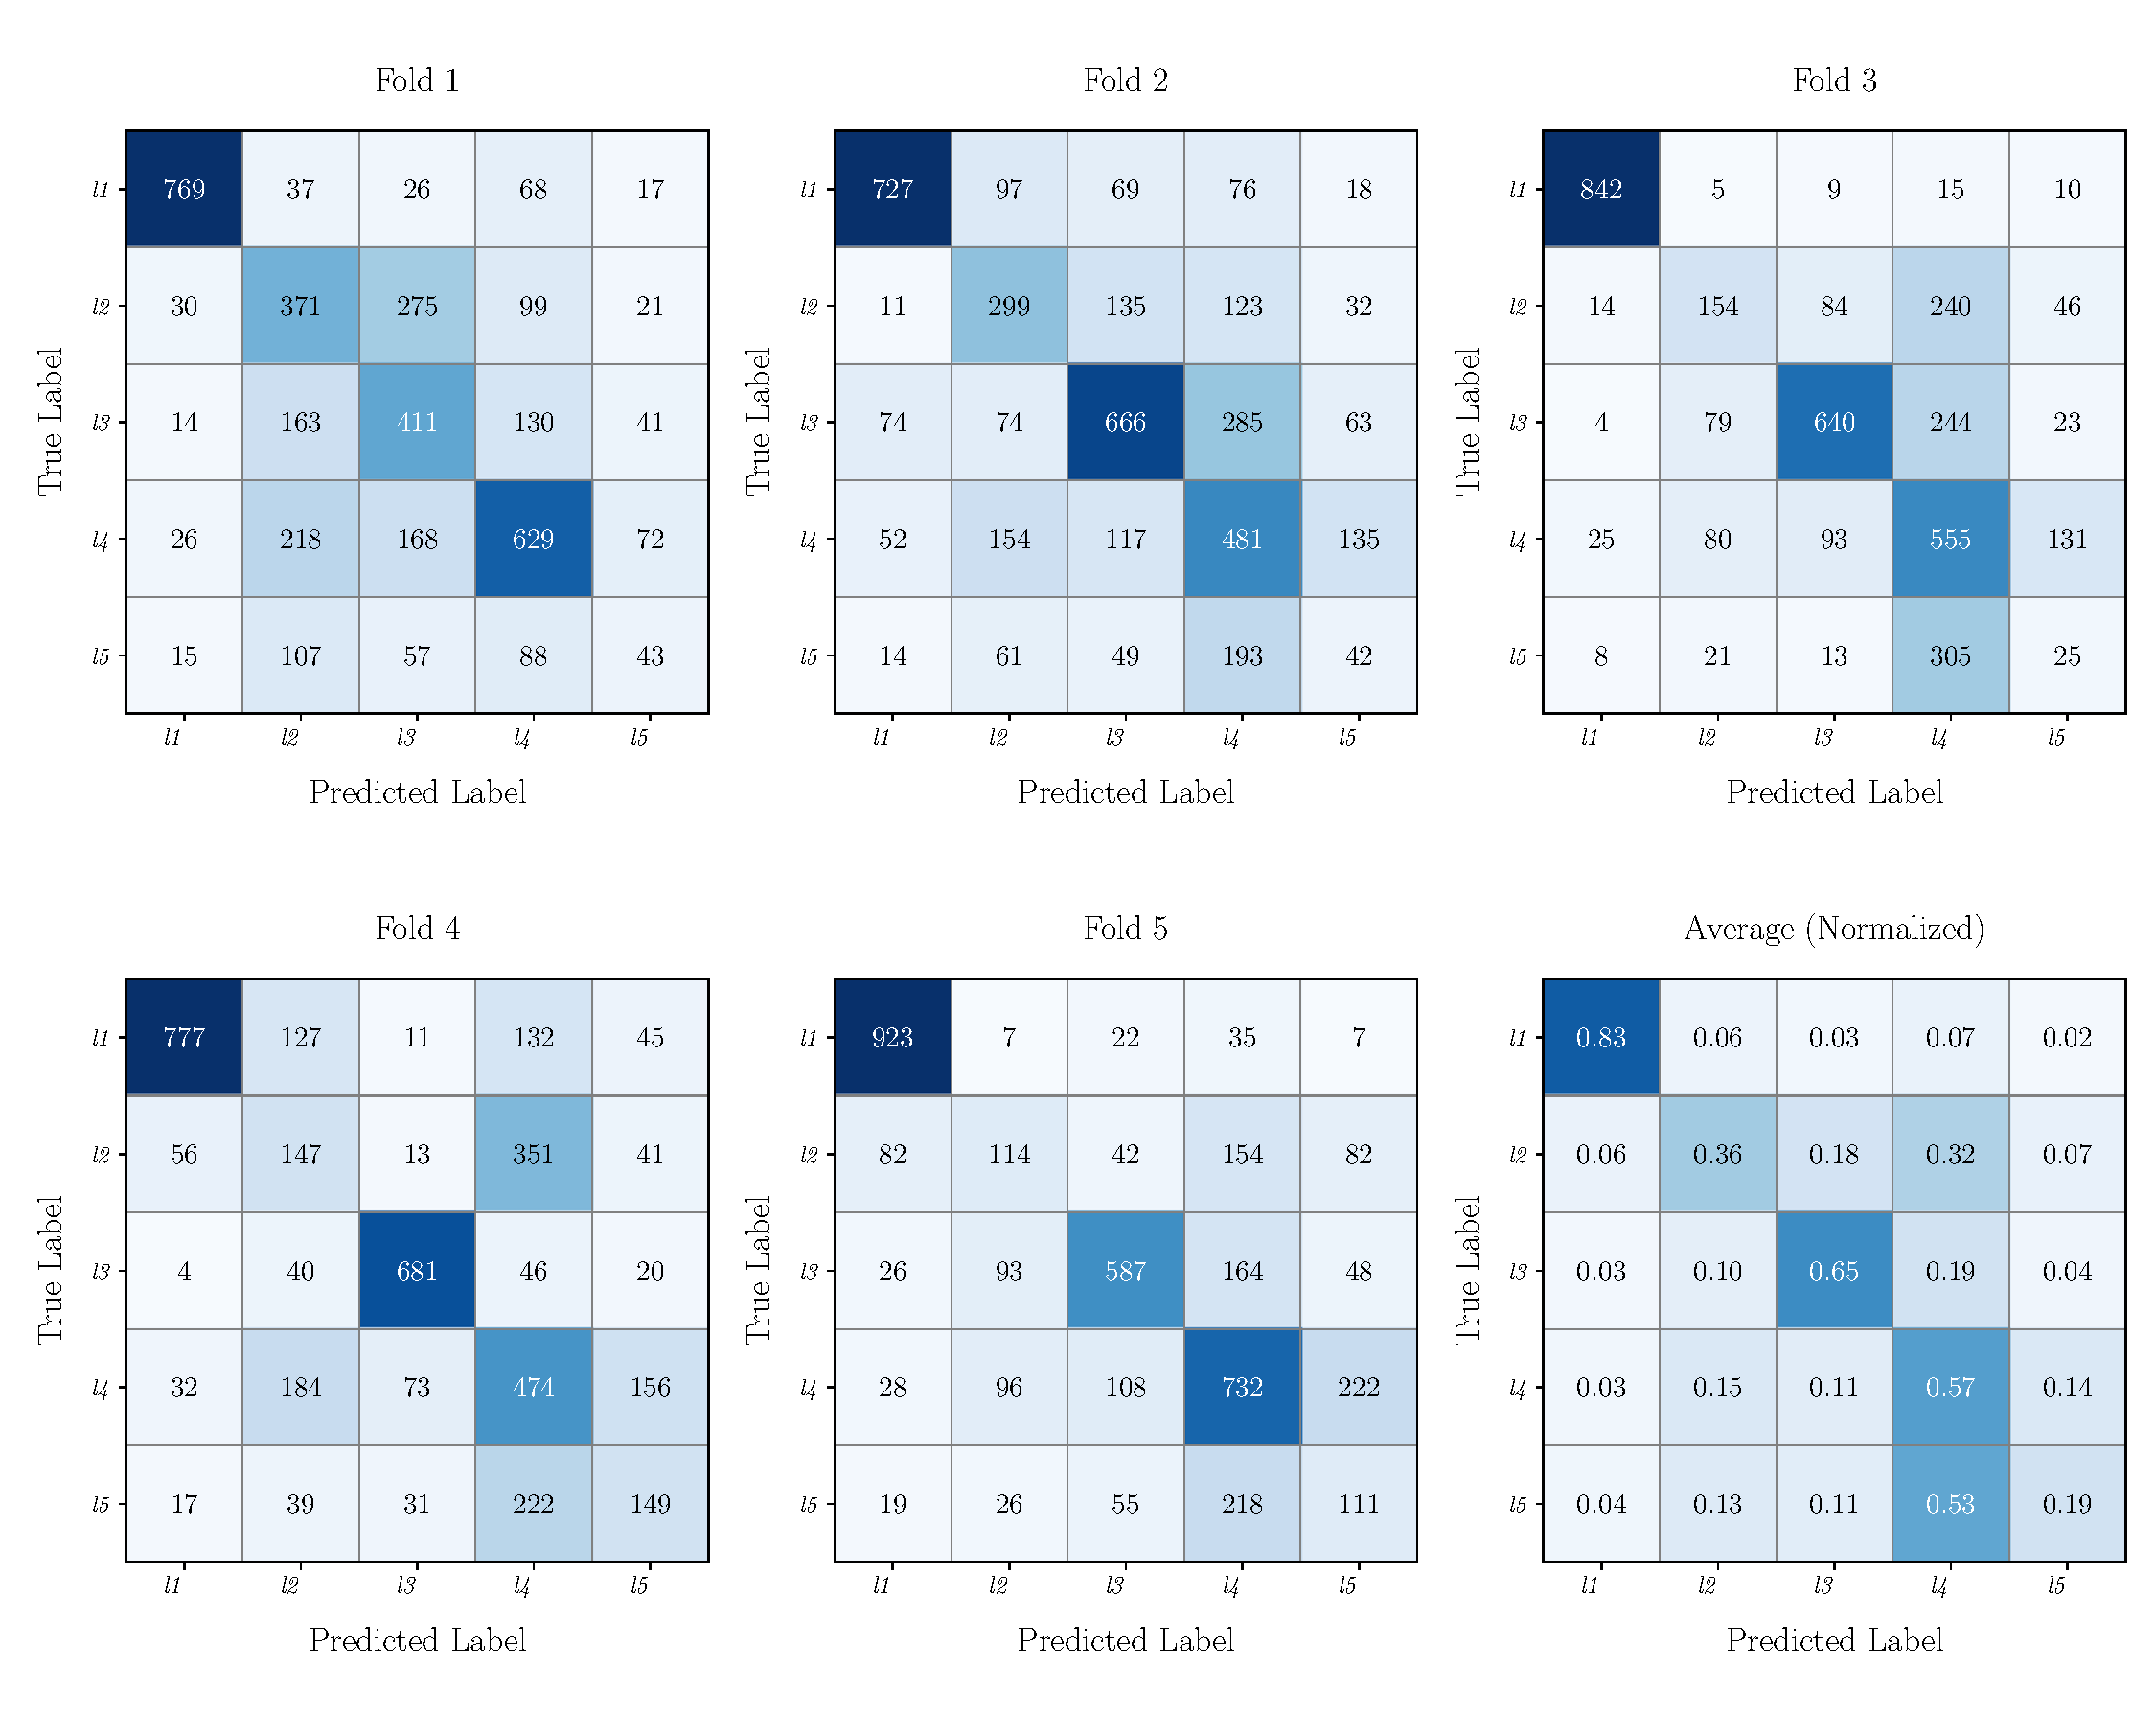
\includegraphics[width=\linewidth]{img/cm_bert.pdf}
%   \caption{BERT}\label{fig:bert_cms}
% \end{subfigure}\hfill
% \begin{subfigure}[b]{0.48\linewidth}
%   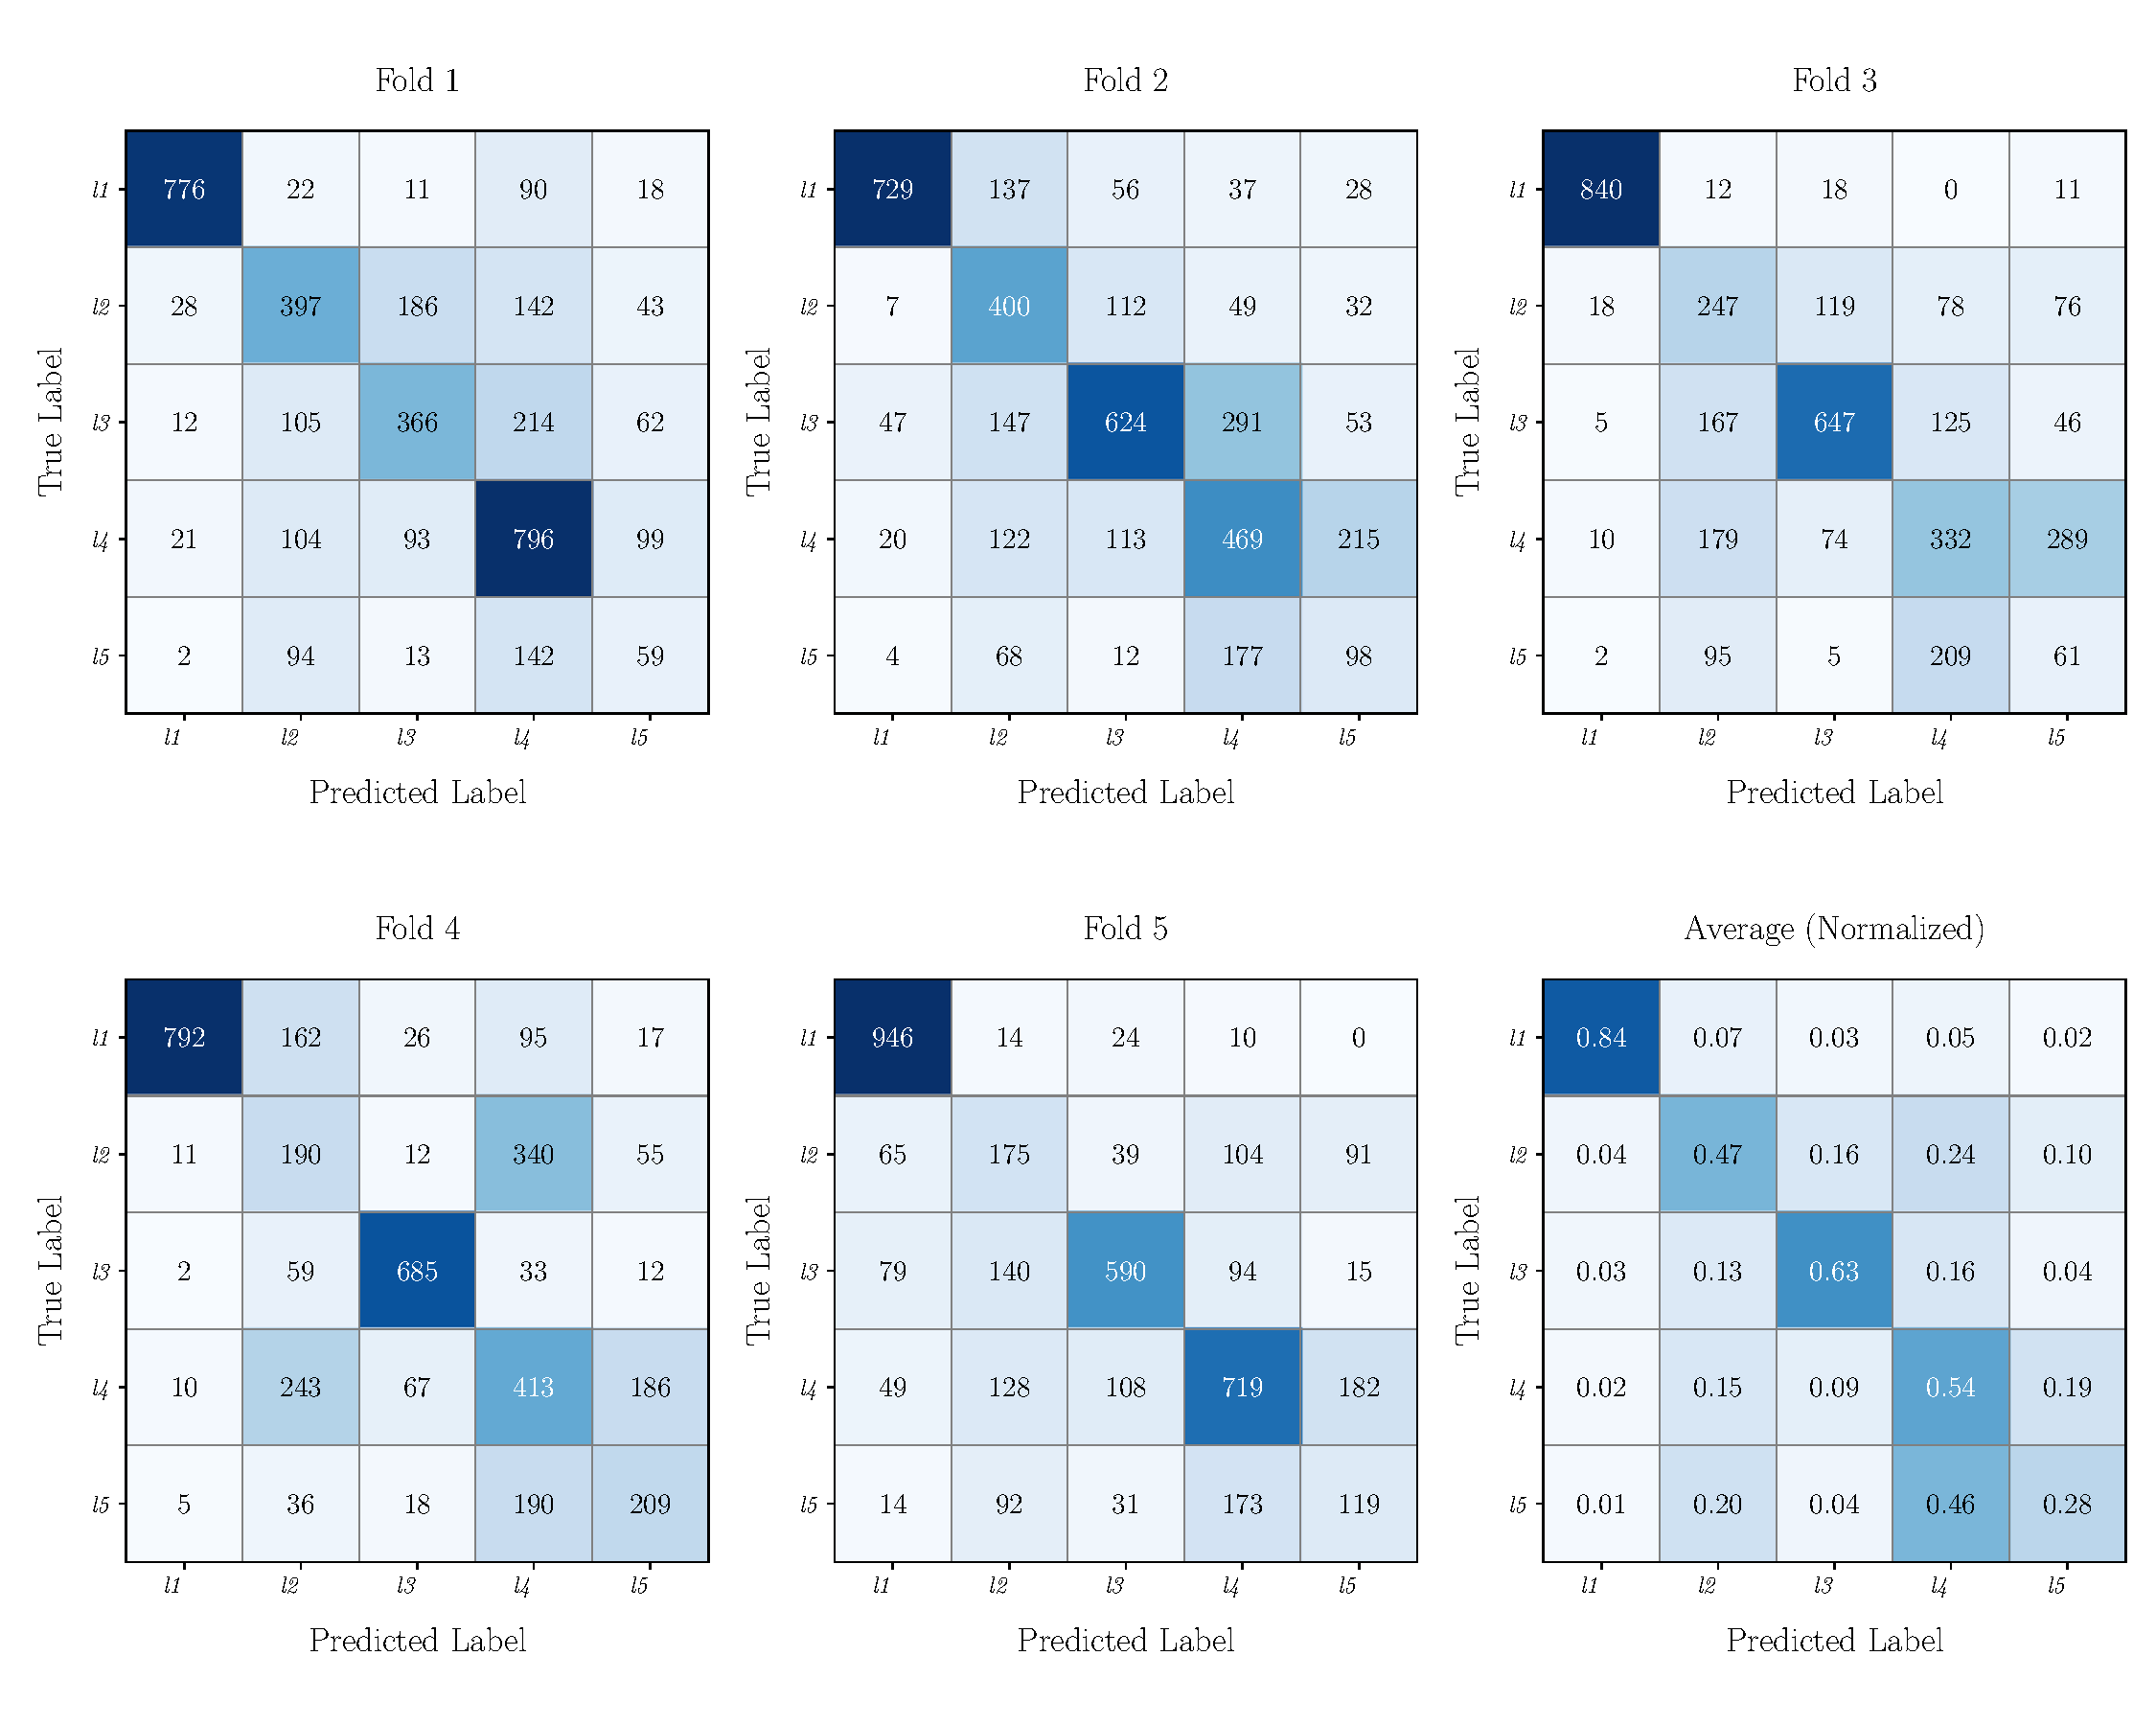
\includegraphics[width=\linewidth]{img/cm_roberta.pdf}
%   \caption{RoBERTa}\label{fig:roberta_cms}
% \end{subfigure}

% \vspace{0.4cm}

% % riga 2
% \begin{subfigure}[b]{0.48\linewidth}
%   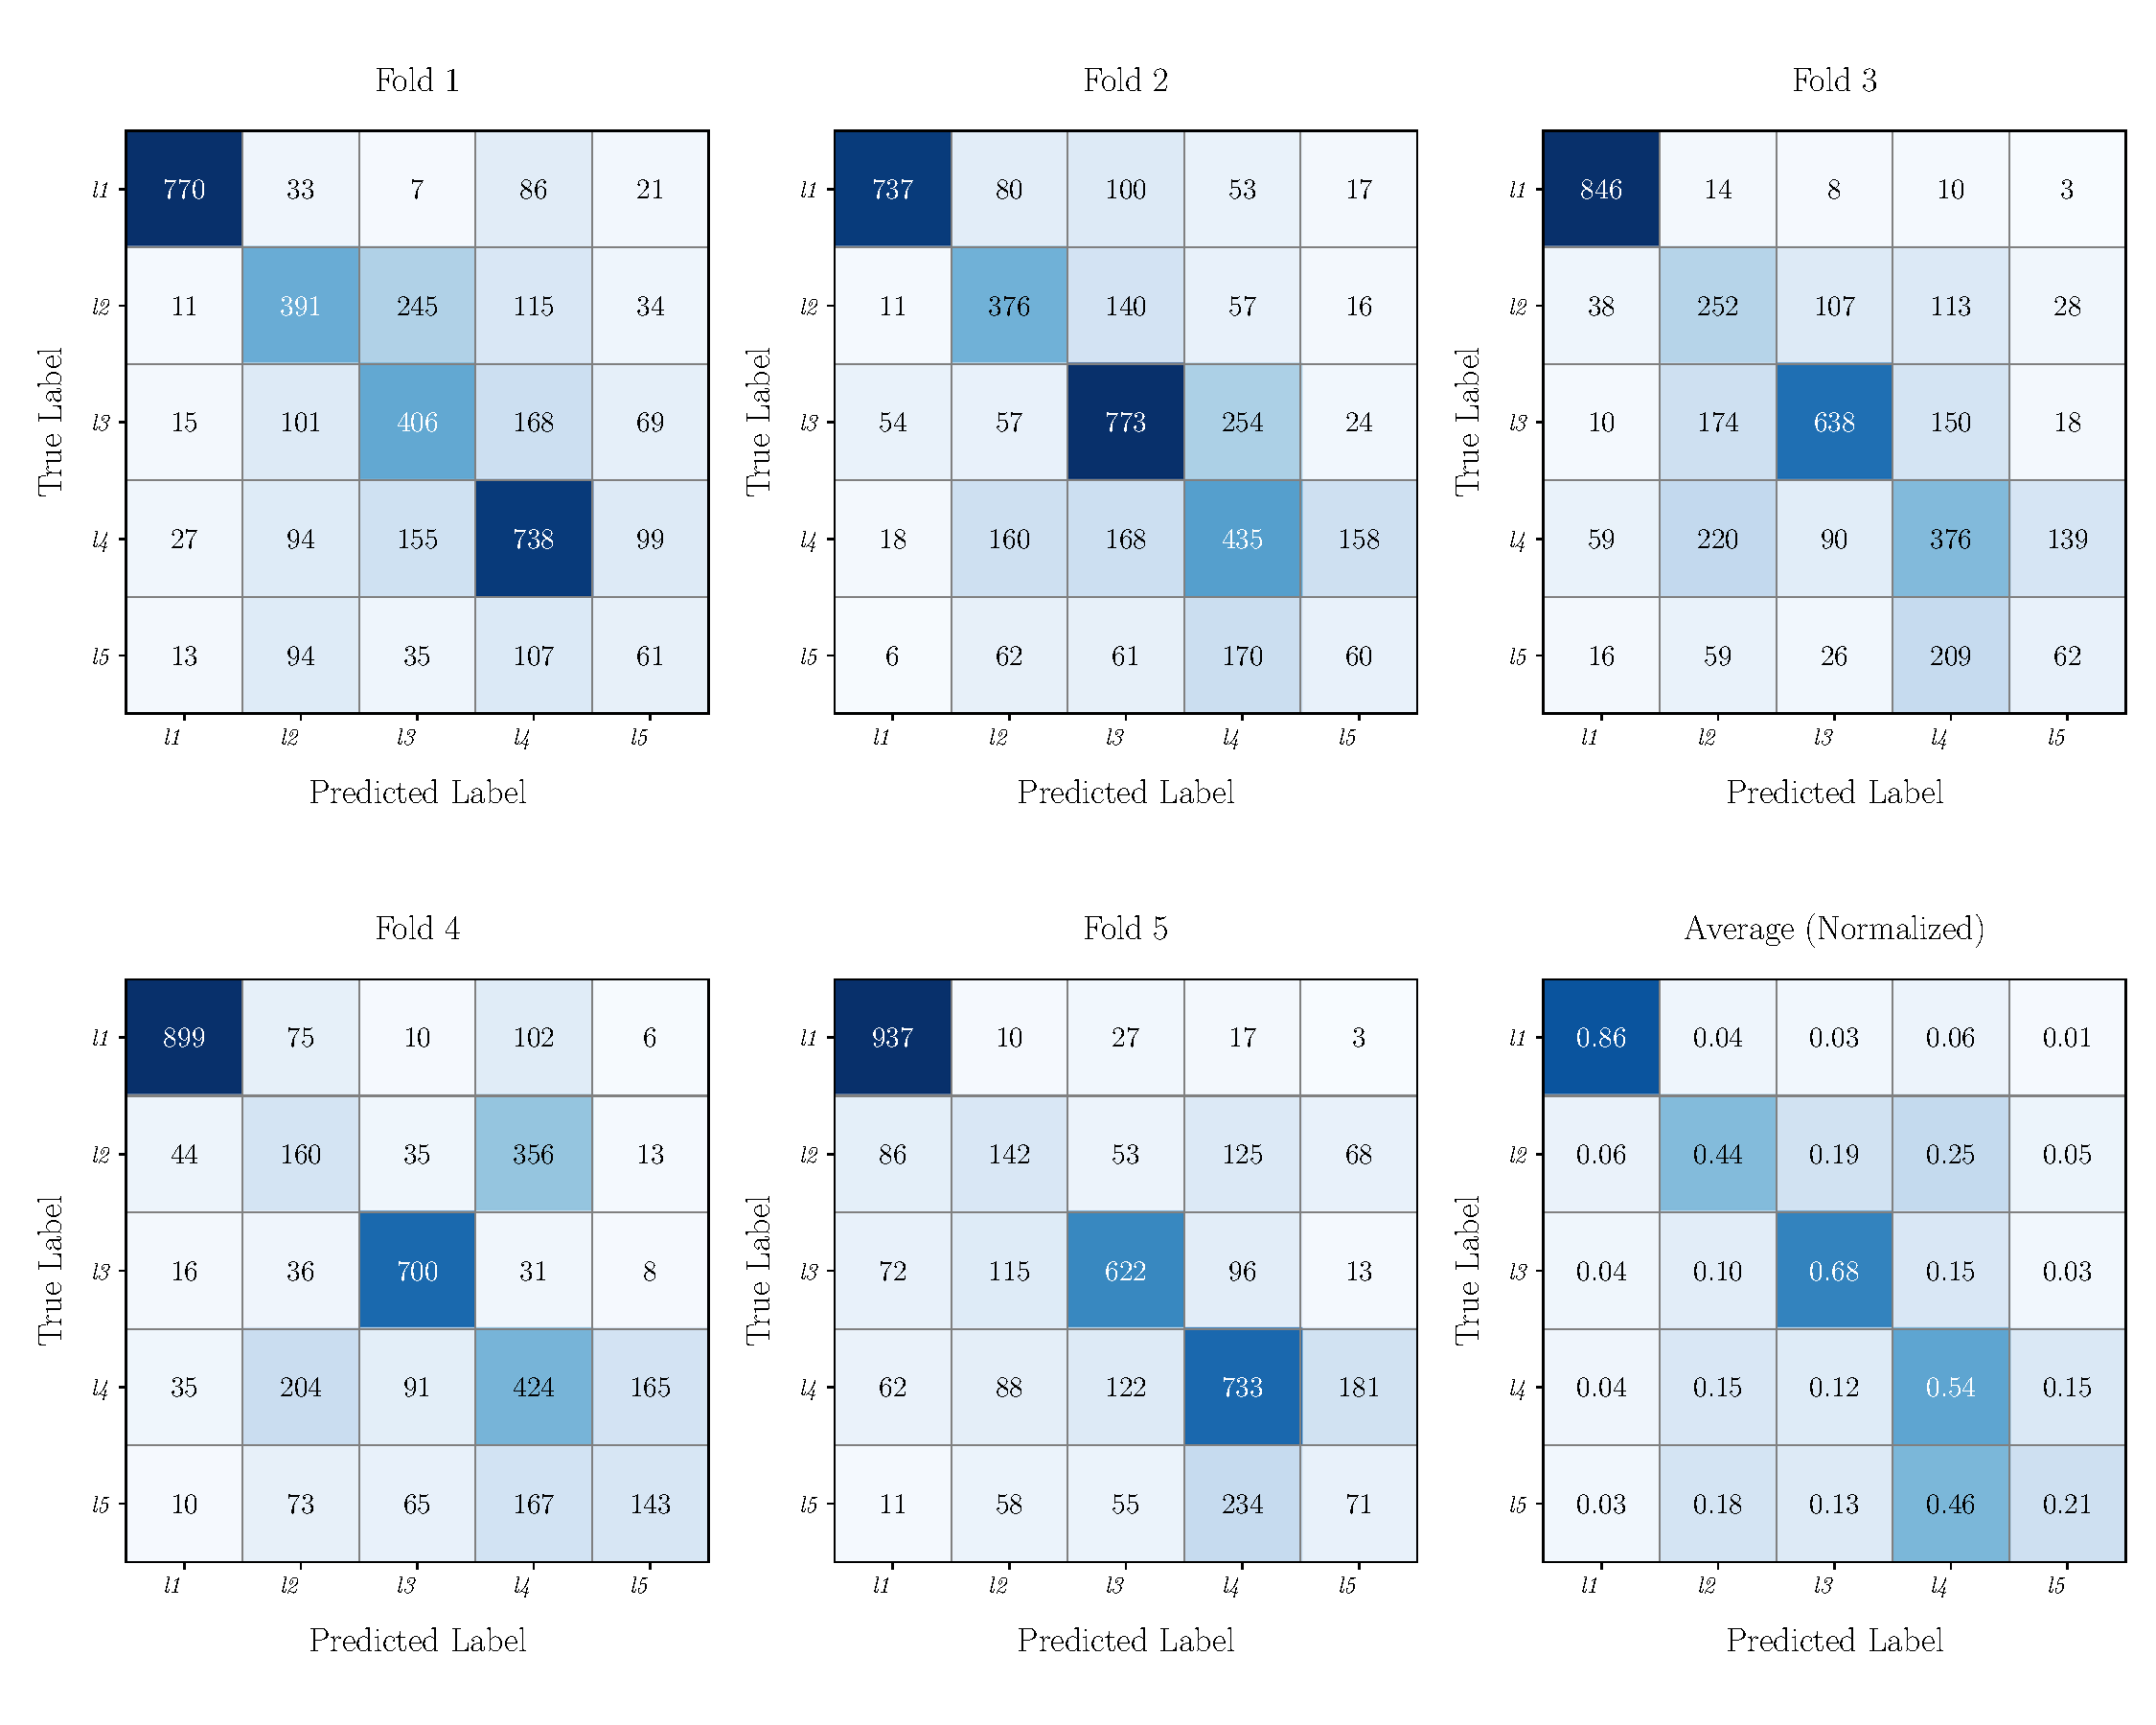
\includegraphics[width=\linewidth]{img/cm_llama.pdf}
%   \caption{Llama 3}\label{fig:llama_cms}
% \end{subfigure}\hfill
% \begin{subfigure}[b]{0.48\linewidth}
%   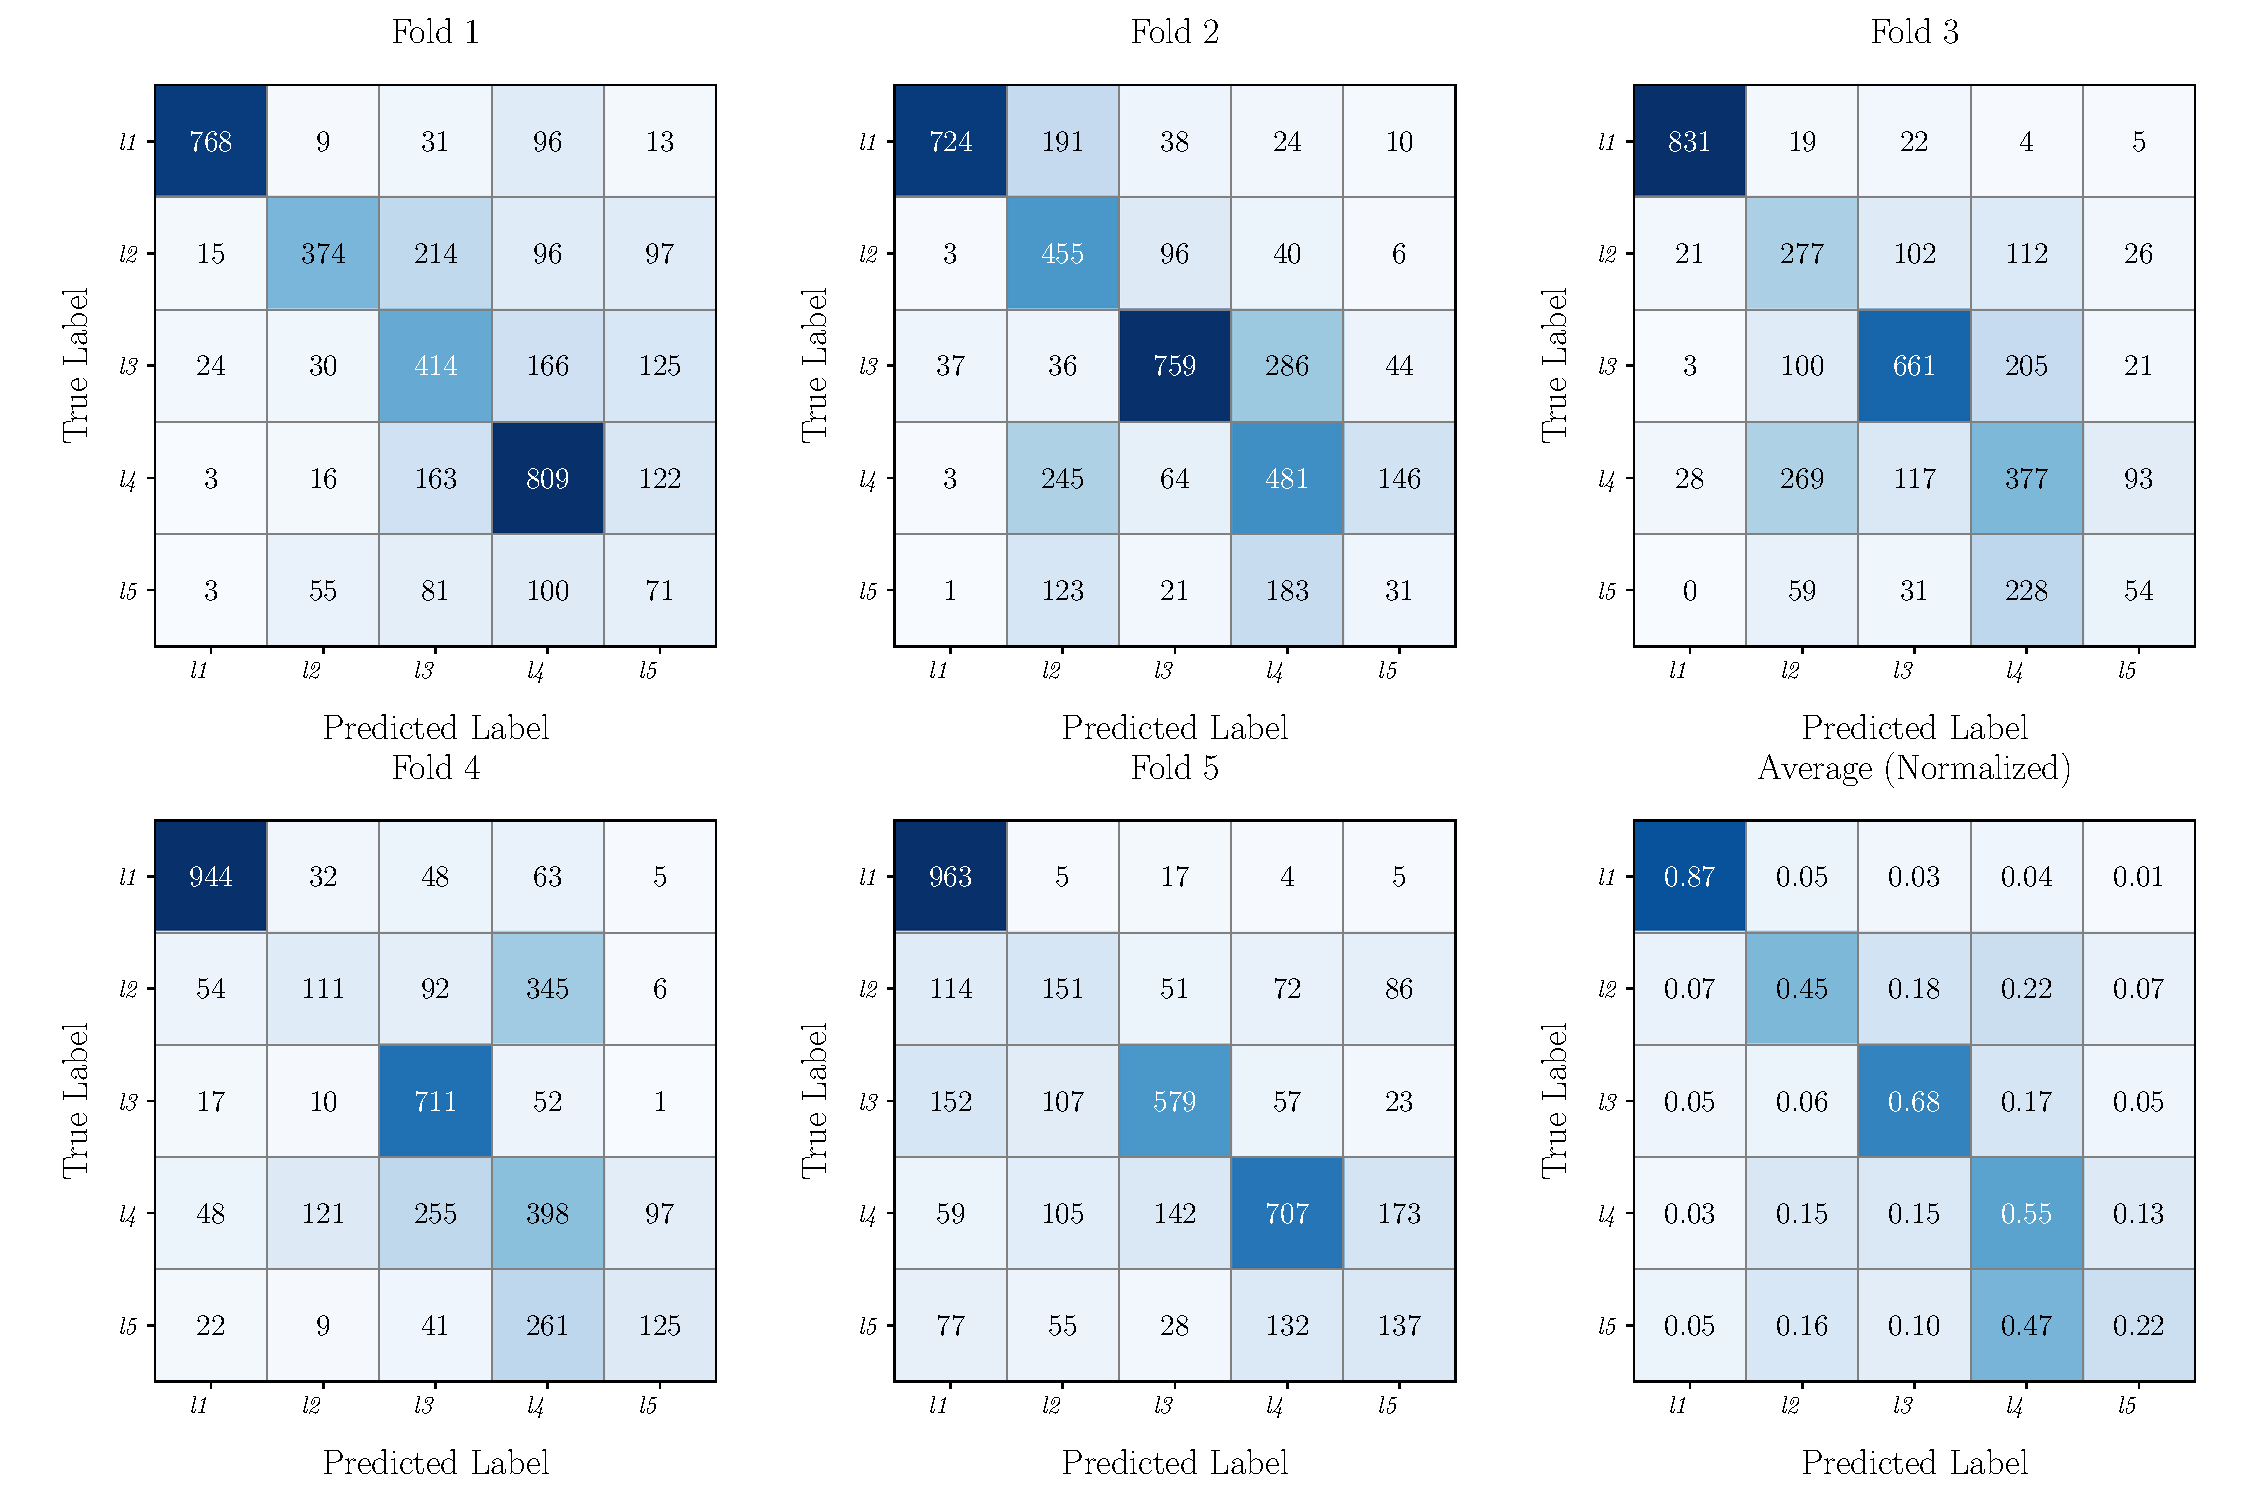
\includegraphics[width=\linewidth]{img/cm_mistral.pdf}
%   \caption{Mistral}\label{fig:mistral_cms}
% \end{subfigure}

% \caption{Confusion matrices showing the models' performance across five cross-validation folds and their overall average. The rows correspond to the true labels and the columns to the predicted ones.}
% \label{fig:performance_cms}
% \end{figure*}

% %%%%%%%%%%%%%%%%%%%%%%%%%%%%%%%%%%%%%%%%%%%%%%%%


% \subsection{Political leaning}
% \label{app:political_cms}

% \begin{figure*}[!t]
% \centering
% % --- riga 1 ---
% \begin{subfigure}[b]{0.48\linewidth}
%   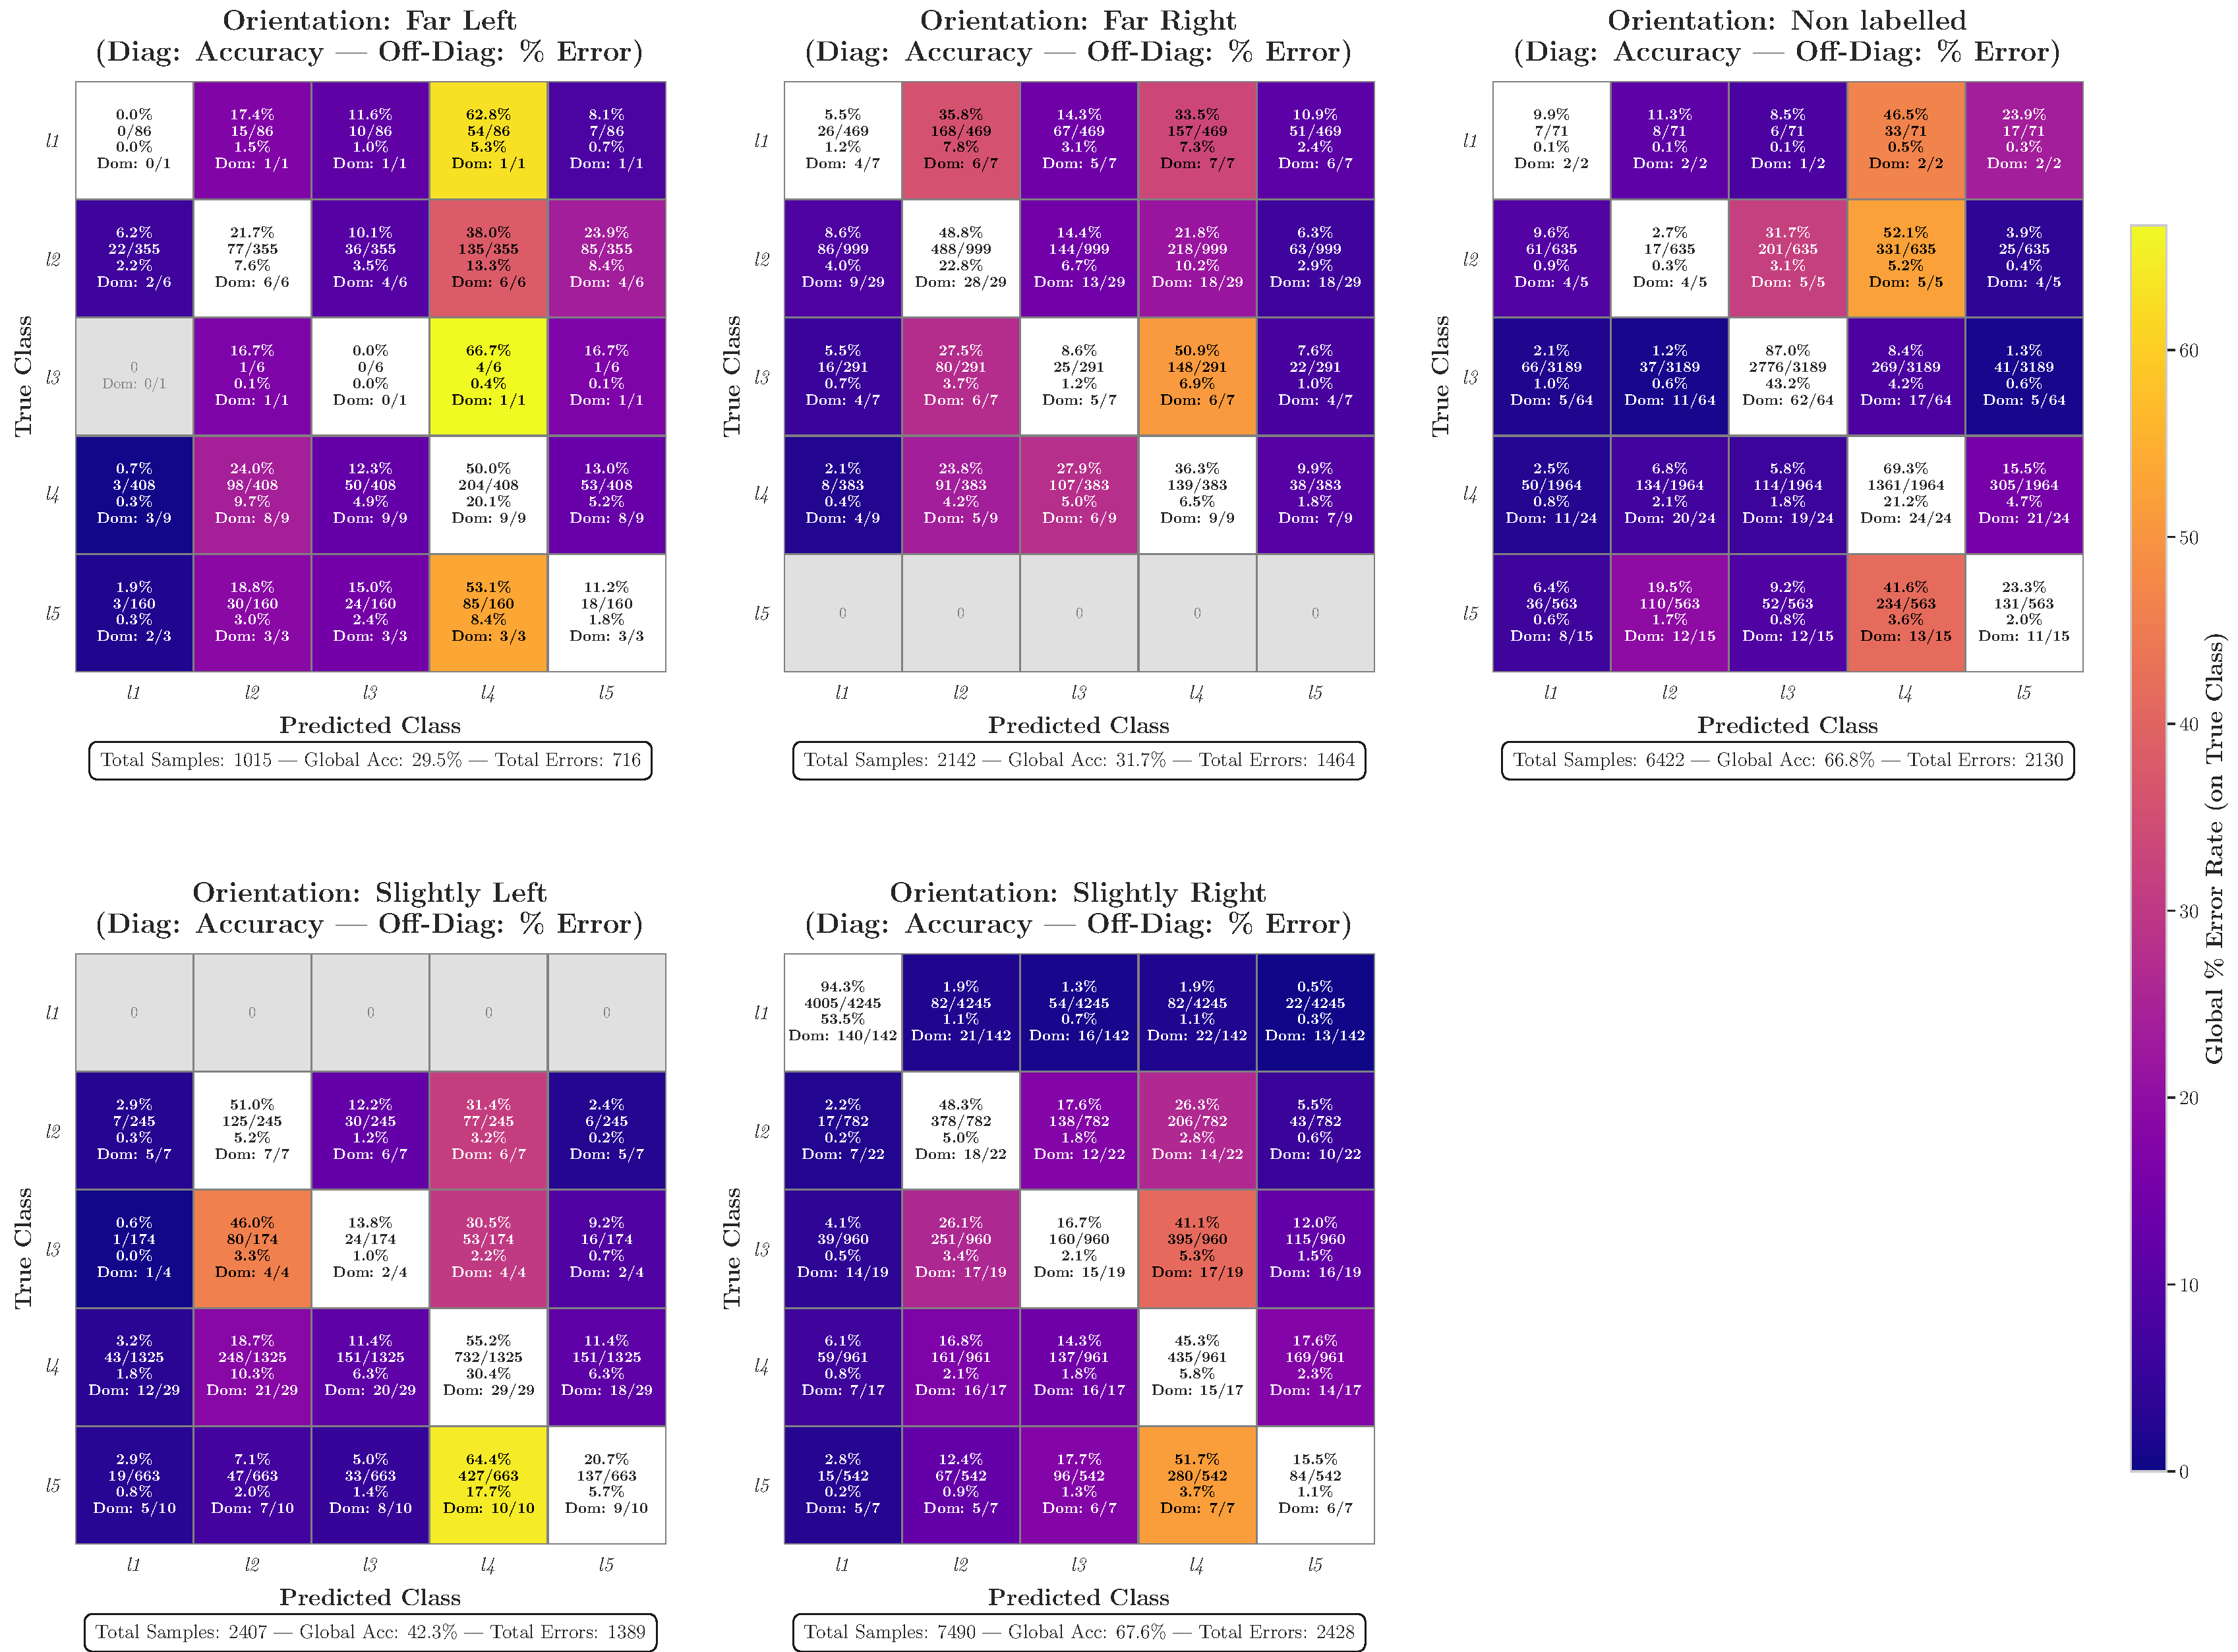
\includegraphics[width=\linewidth]{img/cmOnPoliticalLeaningBert.pdf}
%   \caption{BERT}
%   \label{fig:cmPoliticalLeaningBert}
% \end{subfigure}\hfill
% \begin{subfigure}[b]{0.48\linewidth}
%   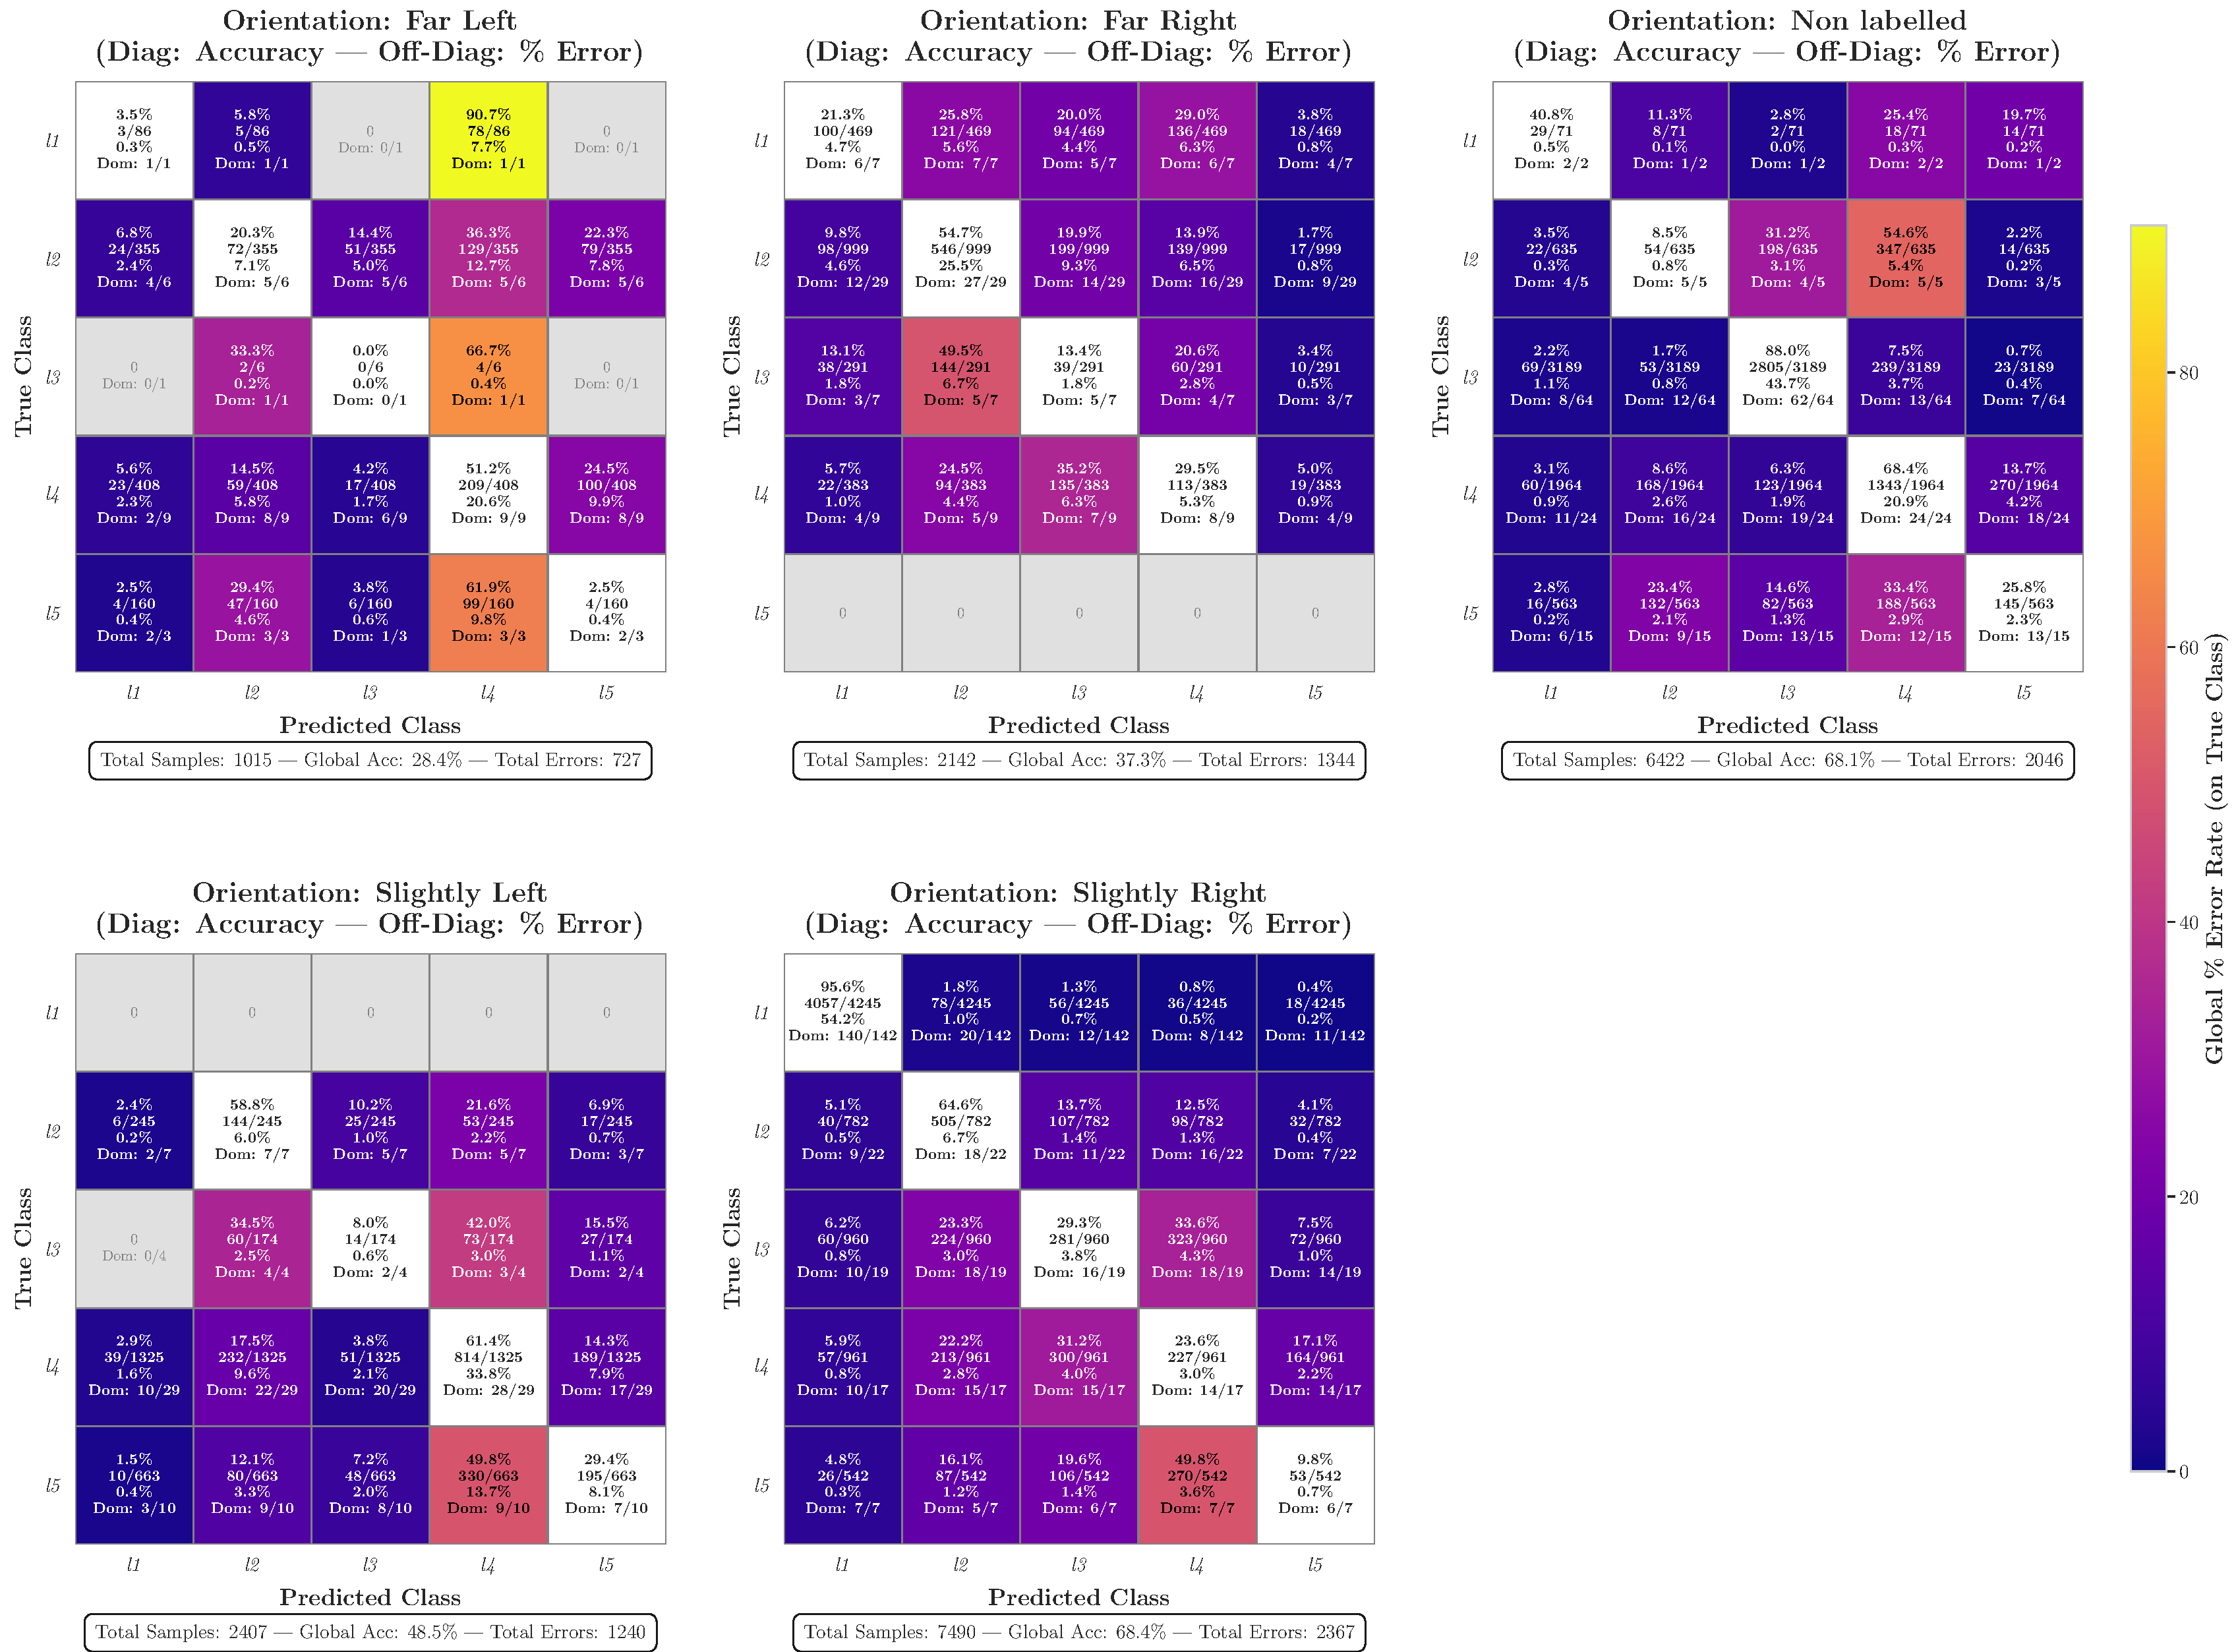
\includegraphics[width=\linewidth]{img/cmOnPoliticalLeaningRoberta.pdf}
%   \caption{RoBERTa}
%   \label{fig:cmPoliticalLeaningRoberta}
% \end{subfigure}

% \vspace{0.5cm}

% % --- riga 2 ---
% \begin{subfigure}[b]{0.48\linewidth}
%   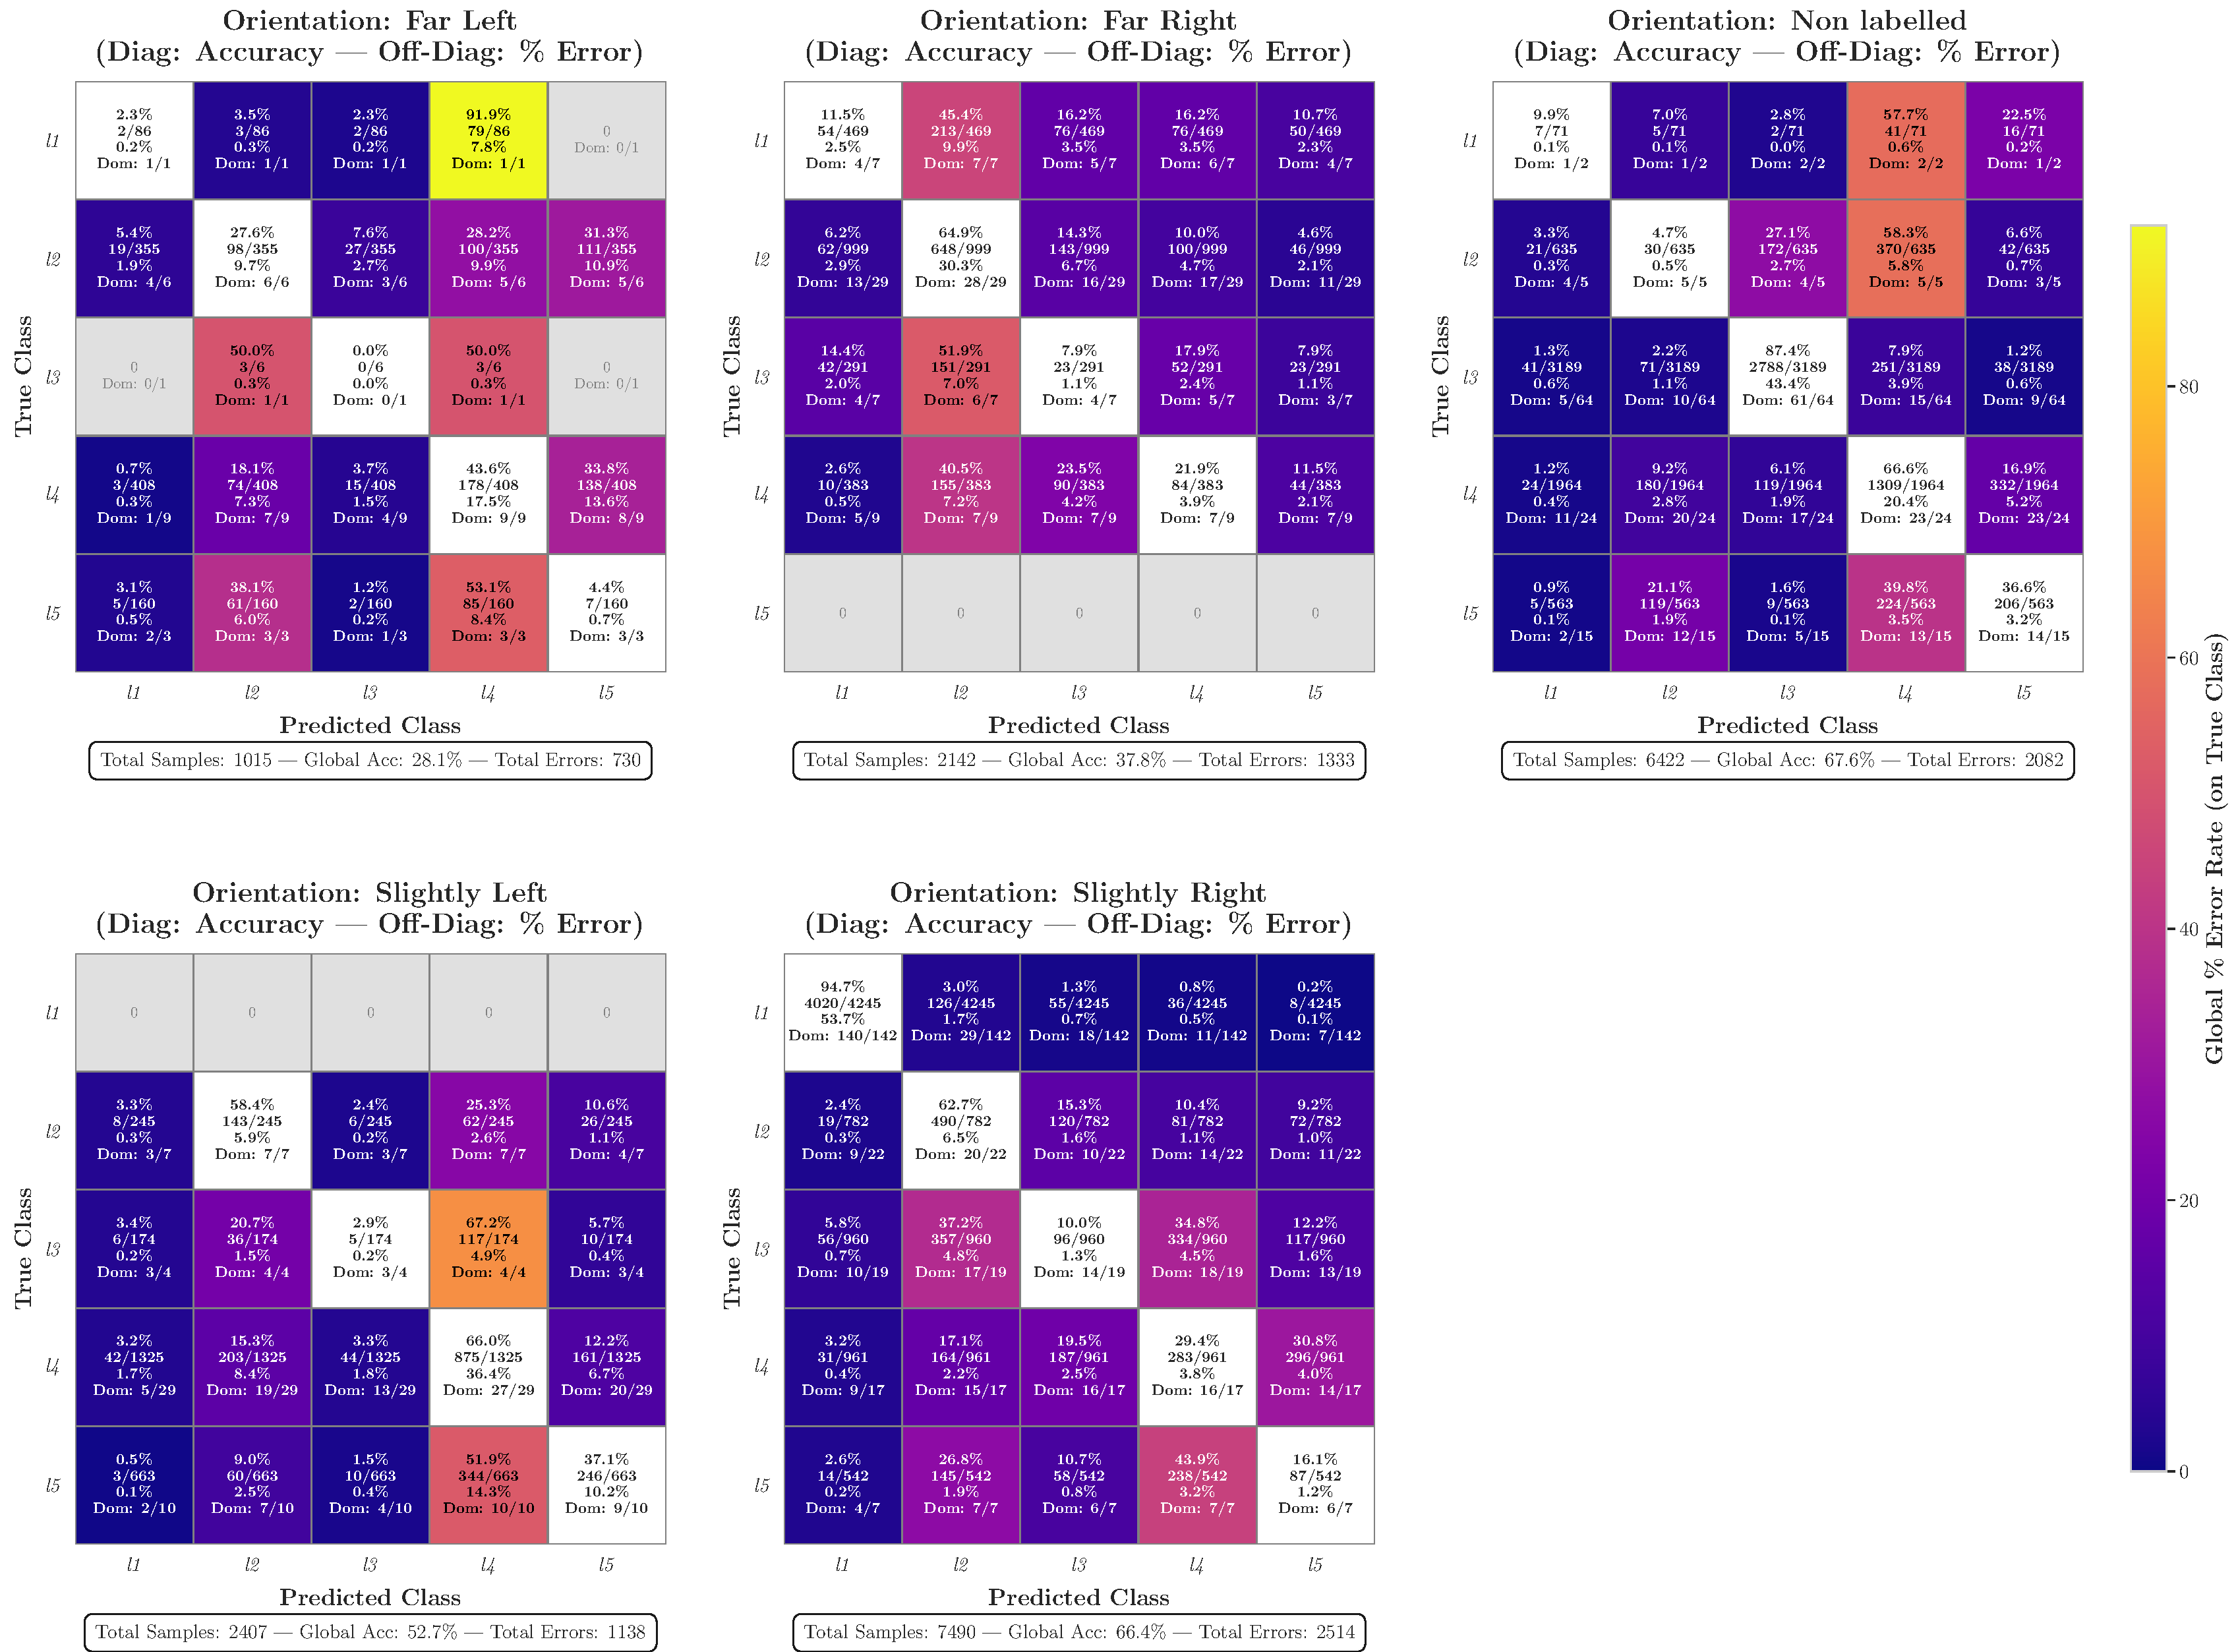
\includegraphics[width=\linewidth]{img/cmOnPoliticalLeaningLLama.pdf}
%   \caption{Llama 3}
%   \label{fig:cmPoliticalLeaningLlama}
% \end{subfigure}\hfill
% \begin{subfigure}[b]{0.48\linewidth}
%   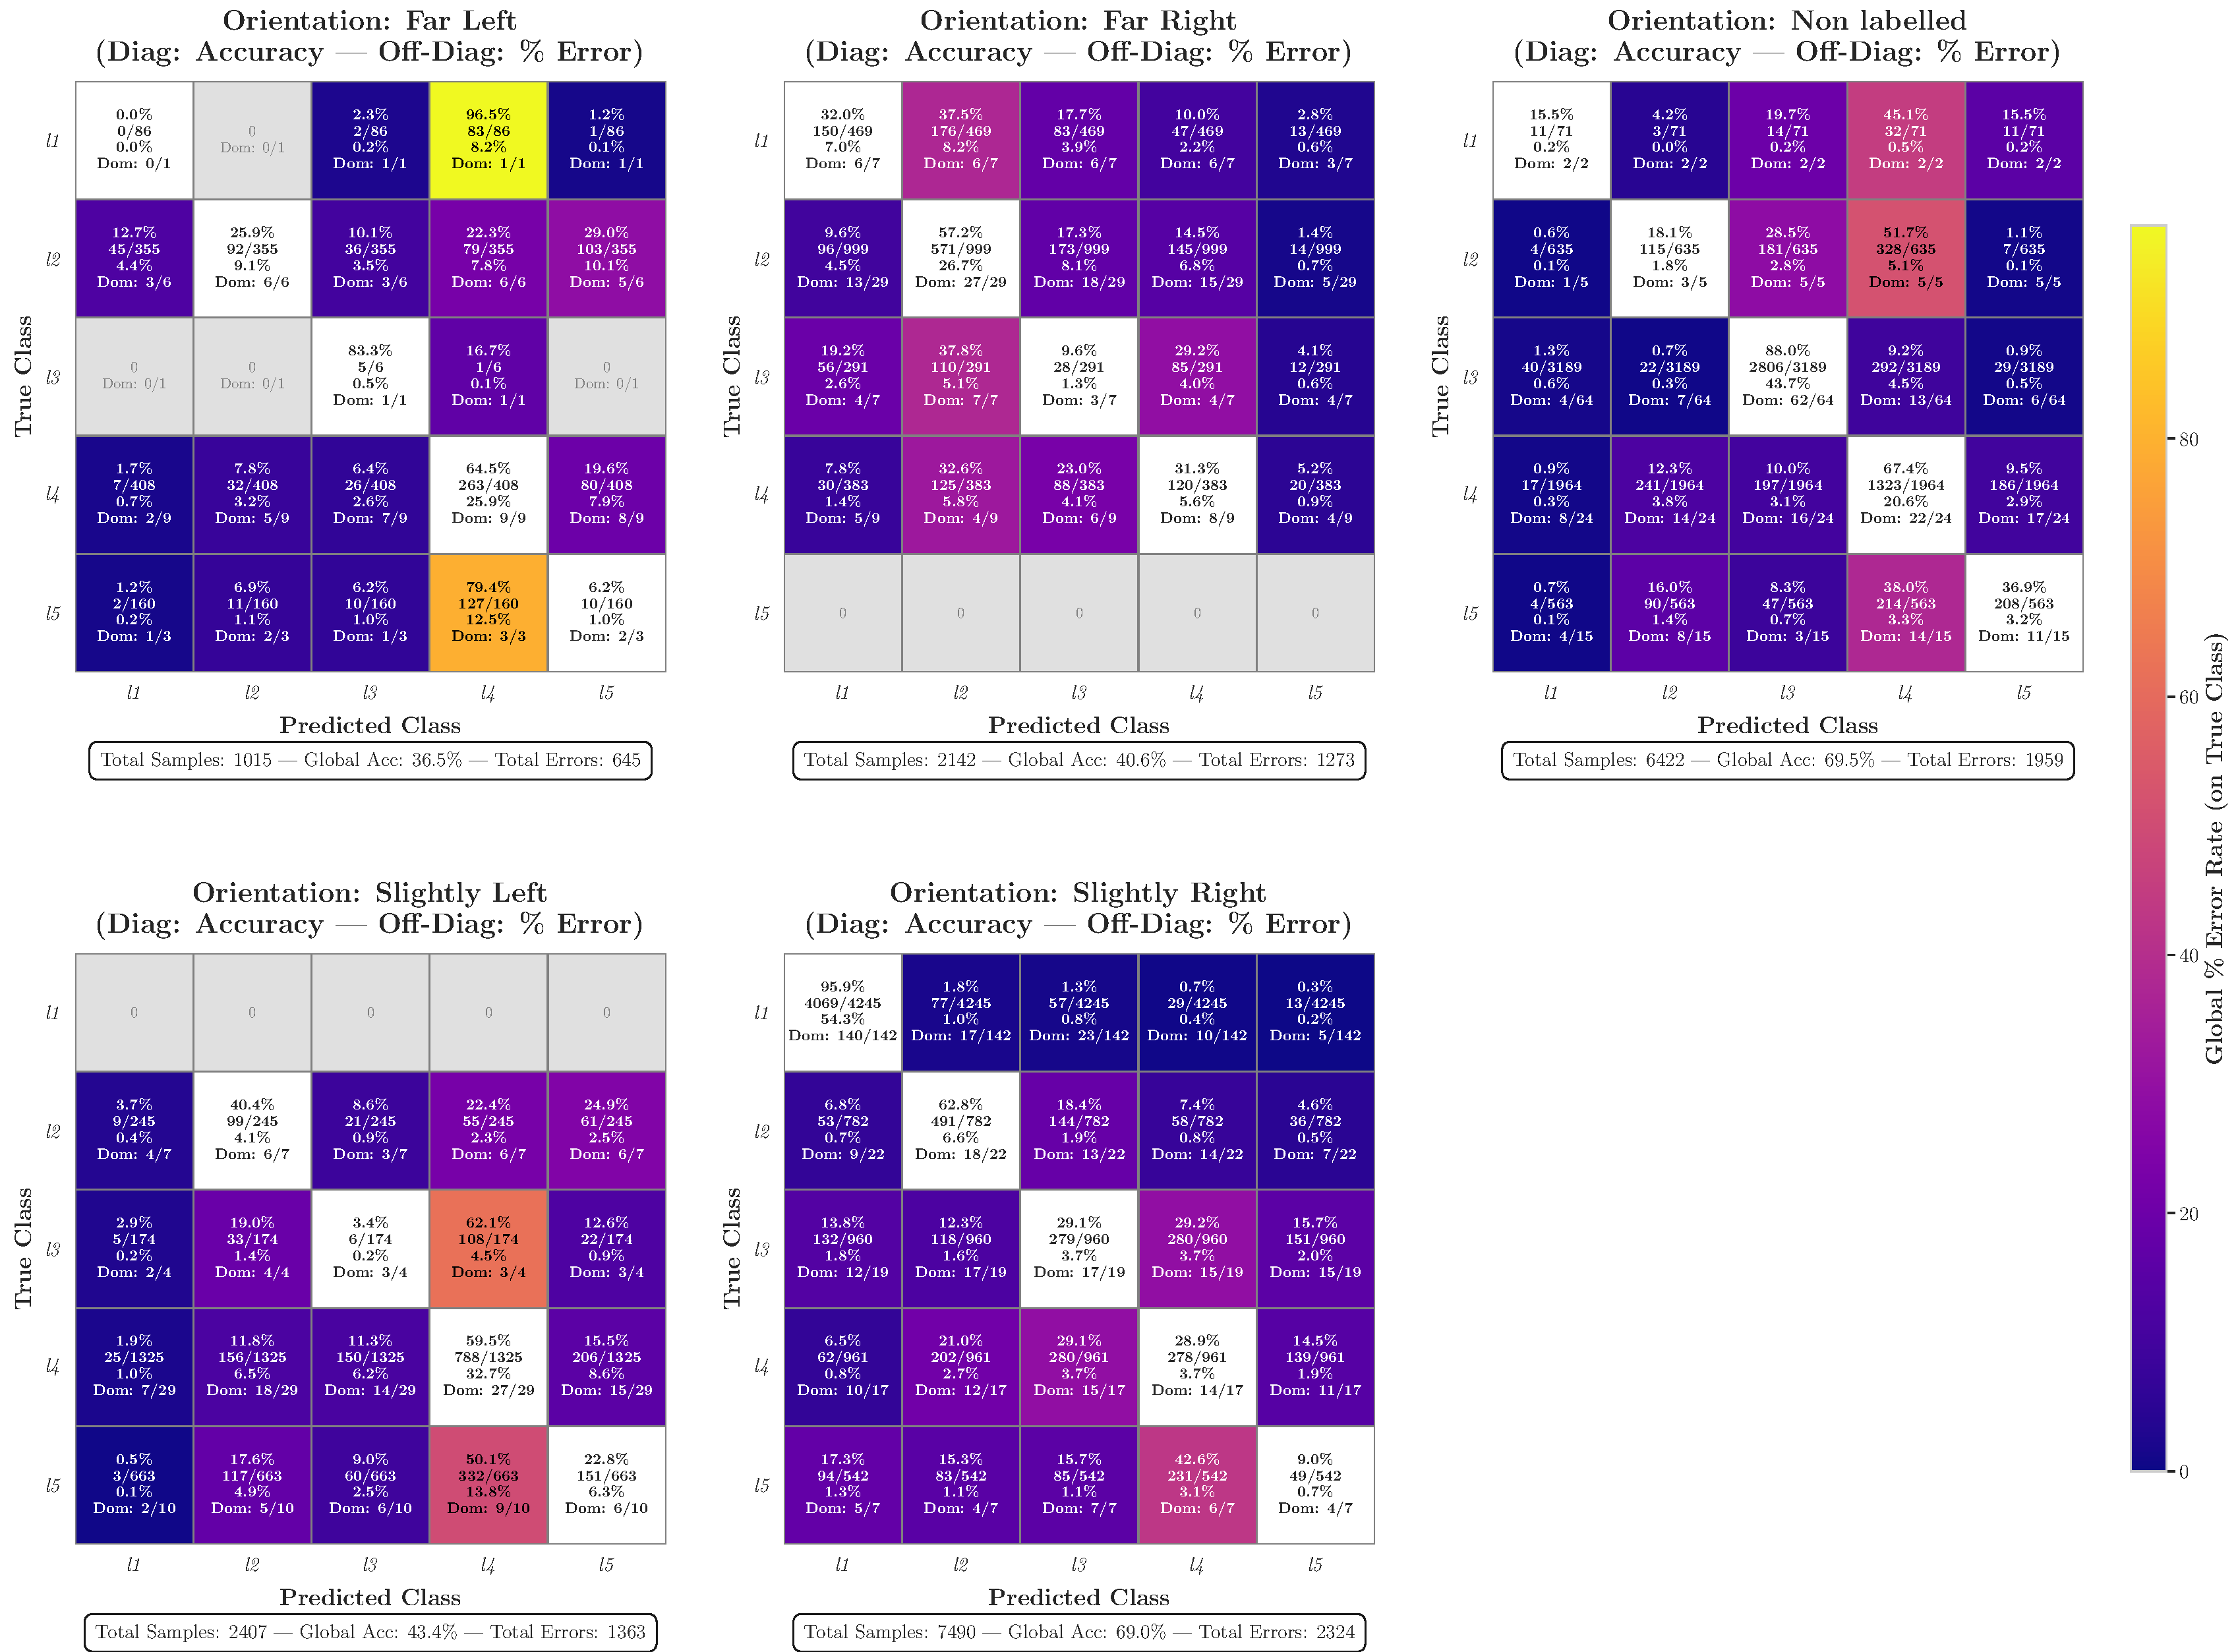
\includegraphics[width=\linewidth]{img/cmOnPoliticalLeaningMistral.pdf}
%   \caption{Mistral}
%   \label{fig:cmPoliticalLeaningMistral}
% \end{subfigure}

% \caption{Confusion matrices for political orientation across the four models. The rows correspond to the true labels and the columns to the predicted ones. The cells show class-wise percentages and counts, dataset-level percentages and contributing domains, and the colour represents the error rate per true class.}
% \label{fig:cmPoliticalLeaning}
% \end{figure*}



% Figure \ref{fig:cmPoliticalLeaning} reveals why the Chi-square test rejects the hypothesis of independence: the distribution of errors varies between moderate and extreme political groups, with notable differences across models.
% The matrices for `Slightly Right' and `Non-labelled' orientations exhibit strong diagonal dominance across all architectures. For the former (the largest group, $N=7490$), Mistral, RoBERTa, and BERT achieve comparable accuracies of 69.0\%, 68.4\%, and 67.6\%, respectively, with Llama 3 at 66.4\%. The domain counts (annotated as `Dom' in the cells) show that this performance is robust across a large number of unique sources.

% In contrast, the `Far Left' ($N=1015$) and `Far Right' ($N=2142$) matrices display high off-diagonal scattering and significantly lower global accuracy.
% For `Far Left', all models perform poorly with accuracies between 28.1\% and 29.5\% for the three smaller models and 36.5\% for Mistral.
% Visual inspection confirms a systematic directional bias: predictions frequently land in the upper triangle of the matrix, confirming that models overestimate the reliability of these sources.

% The `Far Right' category shows the greatest difference between the models. Mistral, Llama 3, and RoBERTa achieved 40.6\%, 37.8\%, and 37.3\%, respectively, while BERT dropped to 31.7\%.
% %This suggests that Bert is particularly sensitive to the linguistic or editorial features of Far Right outlets in this dataset.


% Domain metrics further clarify that errors in these extreme categories are driven by a small set of outlets. Unlike the diverse `Slightly Right' group, the `Far Left' and `Far Right' categories contain fewer unique domains e.g., \textit{Dom: 1/1} or \textit{Dom: 5/7}, yet these specific outlets consistently trigger model errors.
% The `Slightly Left' matrix confirms the specific discrediting pattern discussed in Section \ref{subsec:politicalBias}.
% A substantial cluster of misclassifications appears in the lower triangle, below the diagonal.
% This visually demonstrates that models penalize these articles, assigning them lower reliability labels compared to the ground truth, a behavior consistent across all the four architectures.

% \subsection{Convergence Analysis}
% \label{app:convergence}
% \textcolor{blue}{This appendix refers to the convergence study that determined the training epochs for the Llama~3 and Mistral models used in the article‑level experiments (Section~\ref{sec:experimental_setup}).}
% To ascertain the most suitable training duration, a preliminary experiment involving 20 epochs was conducted using the Llama 3 model. As can be seen in Figure \ref{fig:loss_plot}, the model converges quickly. The validation loss reaches its minimum at epoch 4 (0.4416), after which the generalisation gap widens, indicating overfitting. The empirical evidence gathered from our most complex architecture validates our decision to limit fine-tuning to five epochs across all models, with the exception noted below.

% We conducted an analogous convergence check for Mistral across the five-fold cross-validation. As can be seen in Figure \ref{fig:loss_mistral}, the training loss decreased sharply from an average of 2.02 at Epoch 1 to 0.36 at Epoch 2 and then to 0.23 at Epoch 3. The average improvement between epochs 2 and 3 is 0.12, indicating diminishing returns and stabilisation. This pattern mirrors the rapid convergence observed for Llama 3, supporting the idea of limiting Mistral training to three epochs to improve efficiency without compromising on convergence.



% \begin{figure*}[!t]
% \centering
% \begin{subfigure}[b]{0.48\linewidth}
%   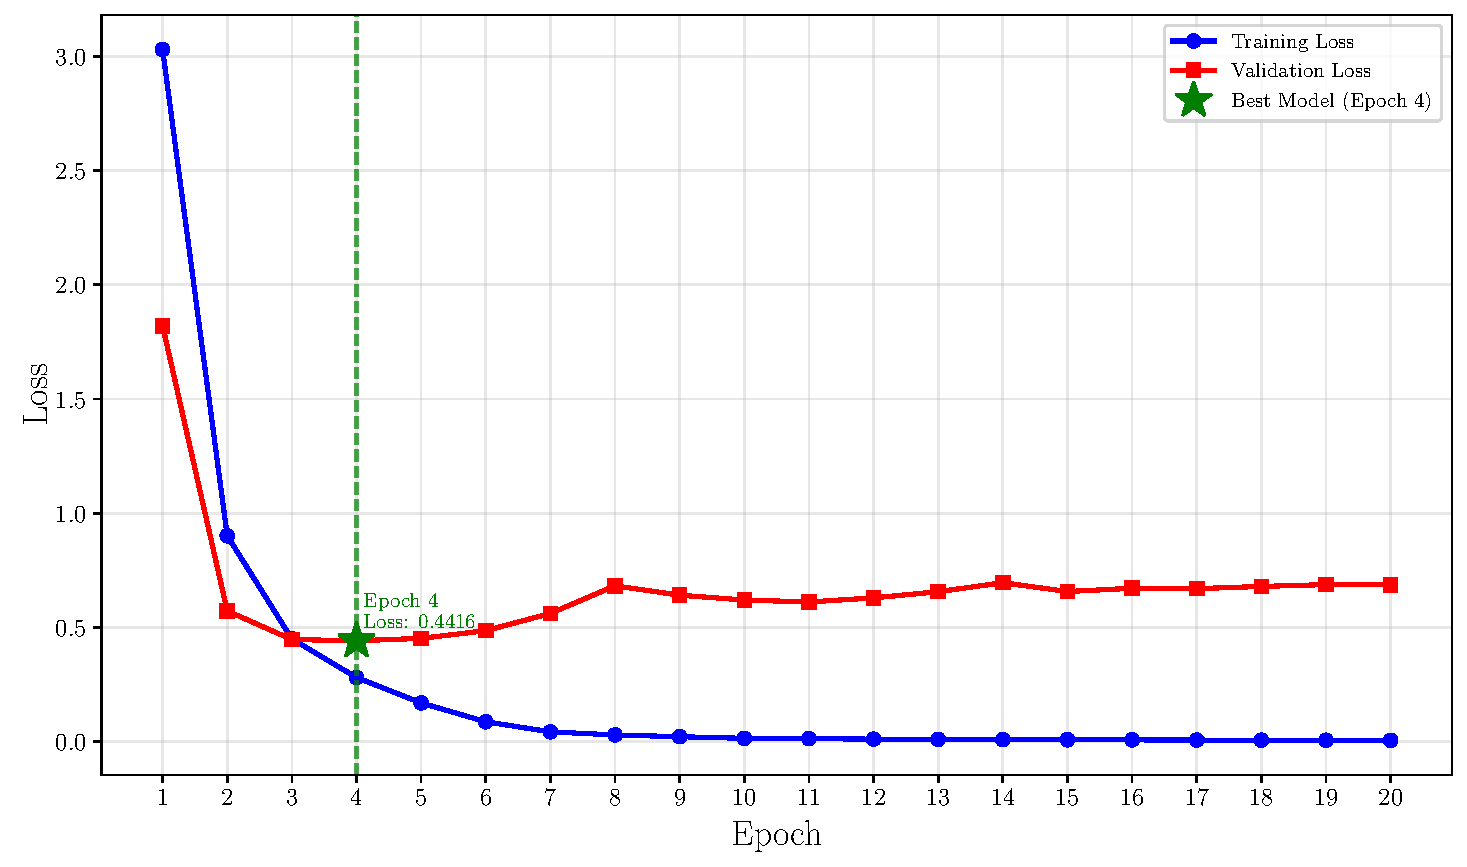
\includegraphics[width=\linewidth]{img/loss_plot.pdf}
%   \caption{Training and Validation loss over 20 epochs for Llama 3. The green marker indicates the optimal model checkpoint at epoch 4. Longer training durations result in poorer generalisation performance.}
%   \label{fig:loss_plot}
% \end{subfigure}\hfill
% \begin{subfigure}[b]{0.48\linewidth}
%   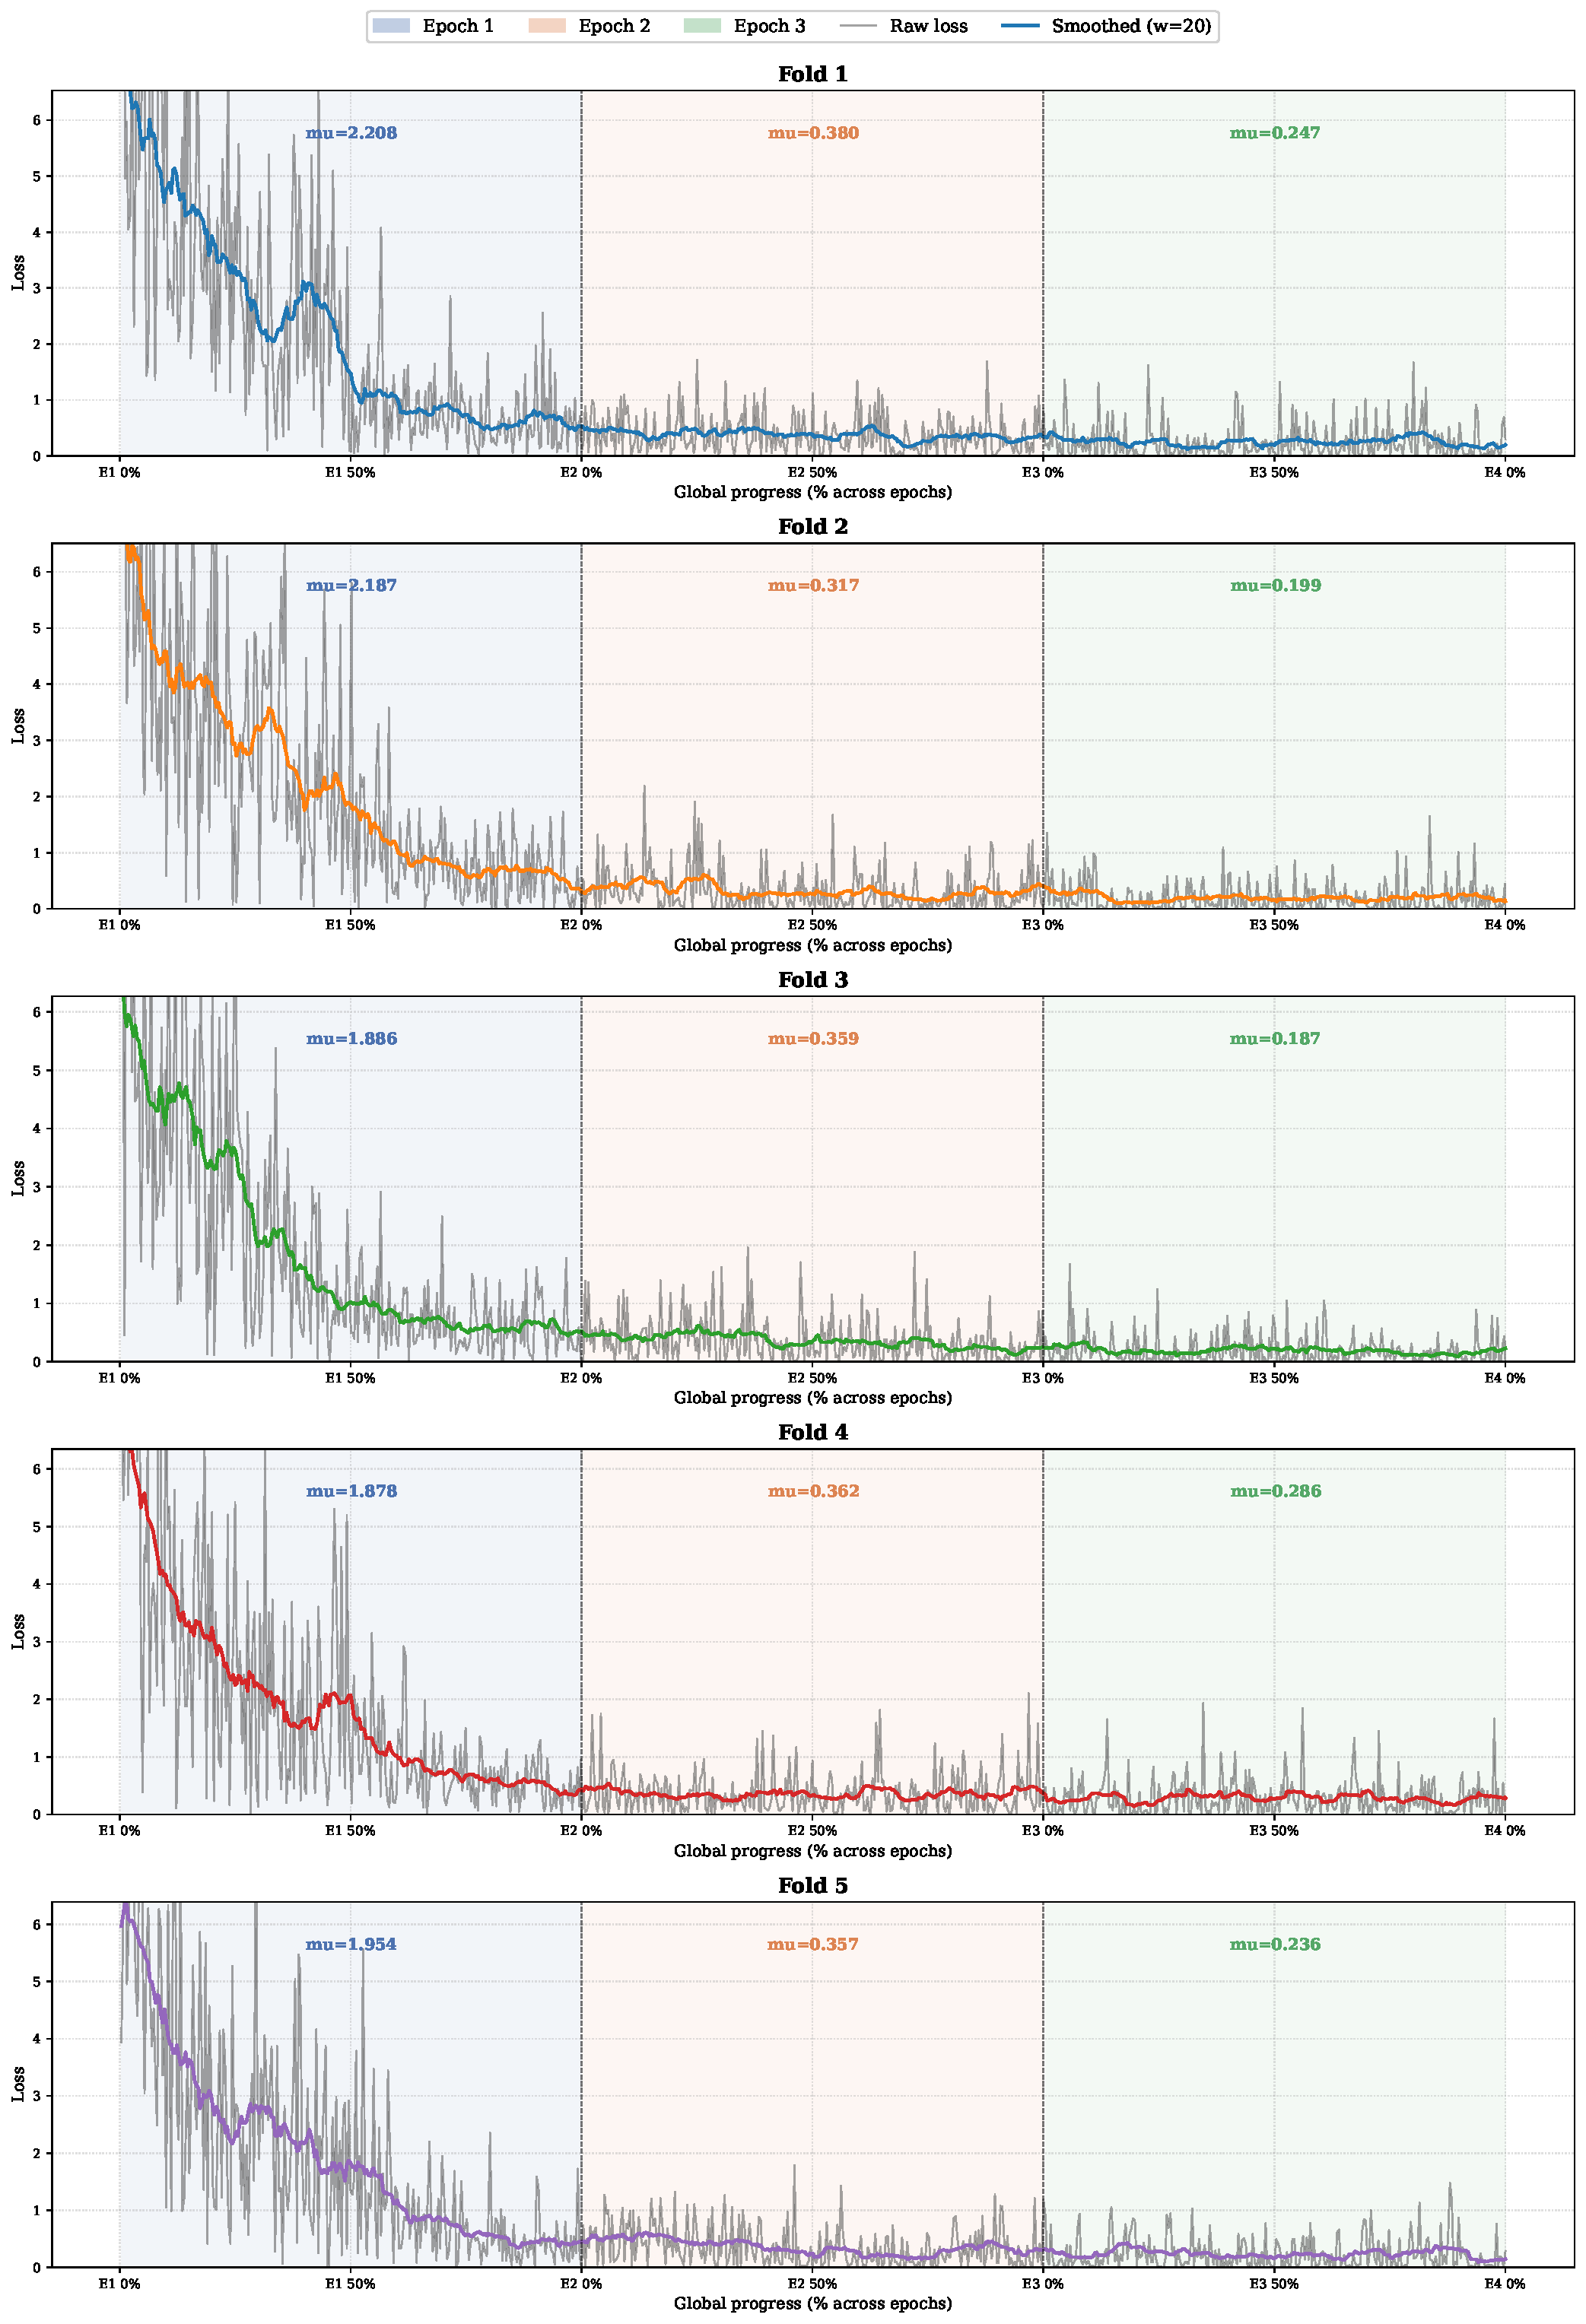
\includegraphics[width=\linewidth]{img/training_loss_mistral.pdf}
%   \caption{Training loss over three epochs for Mistral, shown across five folds. %Each panel represents a cross-validation fold, showing the training dynamics used to assess convergence.
%   }
%   \label{fig:loss_mistral}
% \end{subfigure}
% \end{figure*}










\end{document}




